% Author: Sandy Burden, Version 1
% ----------------------------------------------------------------
% NIASRA Beamer template for Slides *******************************
% ----------------------------------------------------------------
\documentclass{beamer}
%\documentclass[handout]{beamer}
%\pgfpagesuselayout{4 on 1}[a4paper, border shrink=5mm, landscape]

\usepackage{color}
\usepackage{pgfpages}
\usepackage{graphicx}
\usepackage[utf8]{inputenc}
\usepackage[T1]{fontenc}
\usepackage{amsmath,amsthm, amssymb}
\usepackage{amsfonts}
\usepackage{natbib}
\usepackage{bm}
\pdfmapfile{+sansmathaccent.map}

\hfuzz5pt % Don't bother to report over-full boxes < 5pt
\vfuzz5pt % Don't bother to report over-full boxes < 5pt
\setlength{\parskip}{3mm}
\usetheme{NIASRA}

% Include secheader option if you want section headers at top of slide.  Can get wide...
%\usetheme[secheader]{NIASRA}

\newcommand{\Yt}{\widetilde{Y}}                     
\newcommand{\Deltab} {\boldsymbol{\Delta}}
\newcommand{\intd} {\mathrm{d}}                 
\newcommand{\Bmat} {\textbf{B}}                 
\newcommand{\Dmat} {\textbf{D}}
\newcommand{\Qmat} {\textbf{Q}}                 
\newcommand{\Cmat} {\textbf{C}}                 
\newcommand{\cmat} {\textbf{c}}                 
\newcommand{\Imat} {\textbf{I}}                 
\newcommand{\bvec} {\textbf{b}}                 
\newcommand{\svec} {\textbf{s}}                 
\newcommand{\uvec} {\textbf{u}}                 
\newcommand{\omegab} {\boldsymbol {\omega}}     
\newcommand{\s}{\mathbf{s}}                     
\newcommand{\h}{\mathbf{h}}                     
\renewcommand{\b}{\mathbf{b}}                   
\newcommand{\z}{\mathbf{z}}                     
\renewcommand{\v}{\mathbf{v}}                   
\renewcommand{\u}{\mathbf{u}}                   
\newcommand{\w}{\mathbf{w}}                     
\renewcommand{\d}{\mathrm{d}}                   
\newcommand{\Z}{\mathbf{Z}}                     
\newcommand{\x}{\mathbf{x}}                   
\newcommand{\Y}{\mathbf{Y}}                     
\newcommand{\Yvec}{\mathbf{Y}}                  
\newcommand{\Zvec}{\mathbf{Z}}                  
\newcommand{\epsilonb}{\boldsymbol{\varepsilon}}
\newcommand{\bI}{\mathbf{I}}                    
\newcommand{\bB}{\mathbf{B}}                    
\newcommand{\bbeta}{\boldsymbol{\beta}}         
\newcommand{\thetab}{\boldsymbol{\theta}}         
\newcommand{\bzero}{\boldsymbol{0}}             
\newcommand{\bSigma}{\bm{\Sigma}}               
\newcommand{\E}{E}                              
\newcommand{\cov}{\mathrm{cov}}                 
\newcommand{\var}{\mathrm{var}}                 
\newcommand{\tr}{\mathrm{tr}}                   
\newcommand{\diag}{\mathrm{diag}}               
\newcommand{\vect}{\mathrm{vec}}                
\newcommand{\Gau}{\mathrm{Gau}}                 
\newcommand{\RR}{\mathbb{R}}     
\newcommand{\varthetab} {{\boldsymbol{\vartheta}}}
\newcommand{\Dist}{\mathrm{Dist}}

\newcommand{\red}{\textcolor{red}}%
\newcommand{\blue}{\textcolor{blue}}

\bibliographystyle{apa}

\title[Causal Spatial Models]{Causal Spatial Models}
\subtitle{Multivariate models constructed using a conditional approach \\ \emph{--- joint work with Noel Cressie ---}} %Not required if you dont want it
\author{Andrew Zammit-Mangion} %
\date[Goulburn 2015]{Goulburn Fellows Research Meeting \\ 18 March, 2015\\ \vskip0.5cm
  
\includegraphics[height=1cm]{NiasraUowLonghand}} % Substitute date of presentation or include todays date instead. 
\institute[UOW]{National Institute of Applied Statistics Research Australia \\
  University of Wollongong}

\begin{document}

\begin{frame}
\titlepage
\end{frame}

% The following slide provides a table of contents for the presentation.  Include or leave out as required.  Additional contents for individual sections can be included throughout the presentation using \tableofcontents[currentsection] or currentsubsection or hideallsubsections, subsubsectionstyle=hide etc.


\begin{frame}
\frametitle{Outline}
  \begin{minipage}{\textwidth}
    \tableofcontents
  \end{minipage}
\end{frame}

% \frame{\frametitle{Outline}\tableofcontents}


\section{Introduction}

\begin{frame}
\sectionpage
\end{frame}


\subsection{Multivariate models in practice}

% ###################

\begin{frame}
\frametitle{Introduction}

\begin{itemize}
\item {\bf Univariate} spatial model. \vfill

\item {\bf Multivariate} spatial model.
\begin{itemize}
    \item Two or more interacting spatial variables.
    \item Improve prediction on one of the variates by observing the others: {\bf Cokriging}.
    \item Determine which variate caused the observed phenomenon: {\bf Source separation}.
\end{itemize}\vfill
\end{itemize}

\end{frame}

% ###################

\begin{frame}
\frametitle{Example 1: Ozone vs MaxT}

\cite{RoyleBerliner1999}, Midwestern USA.

\begin{center}
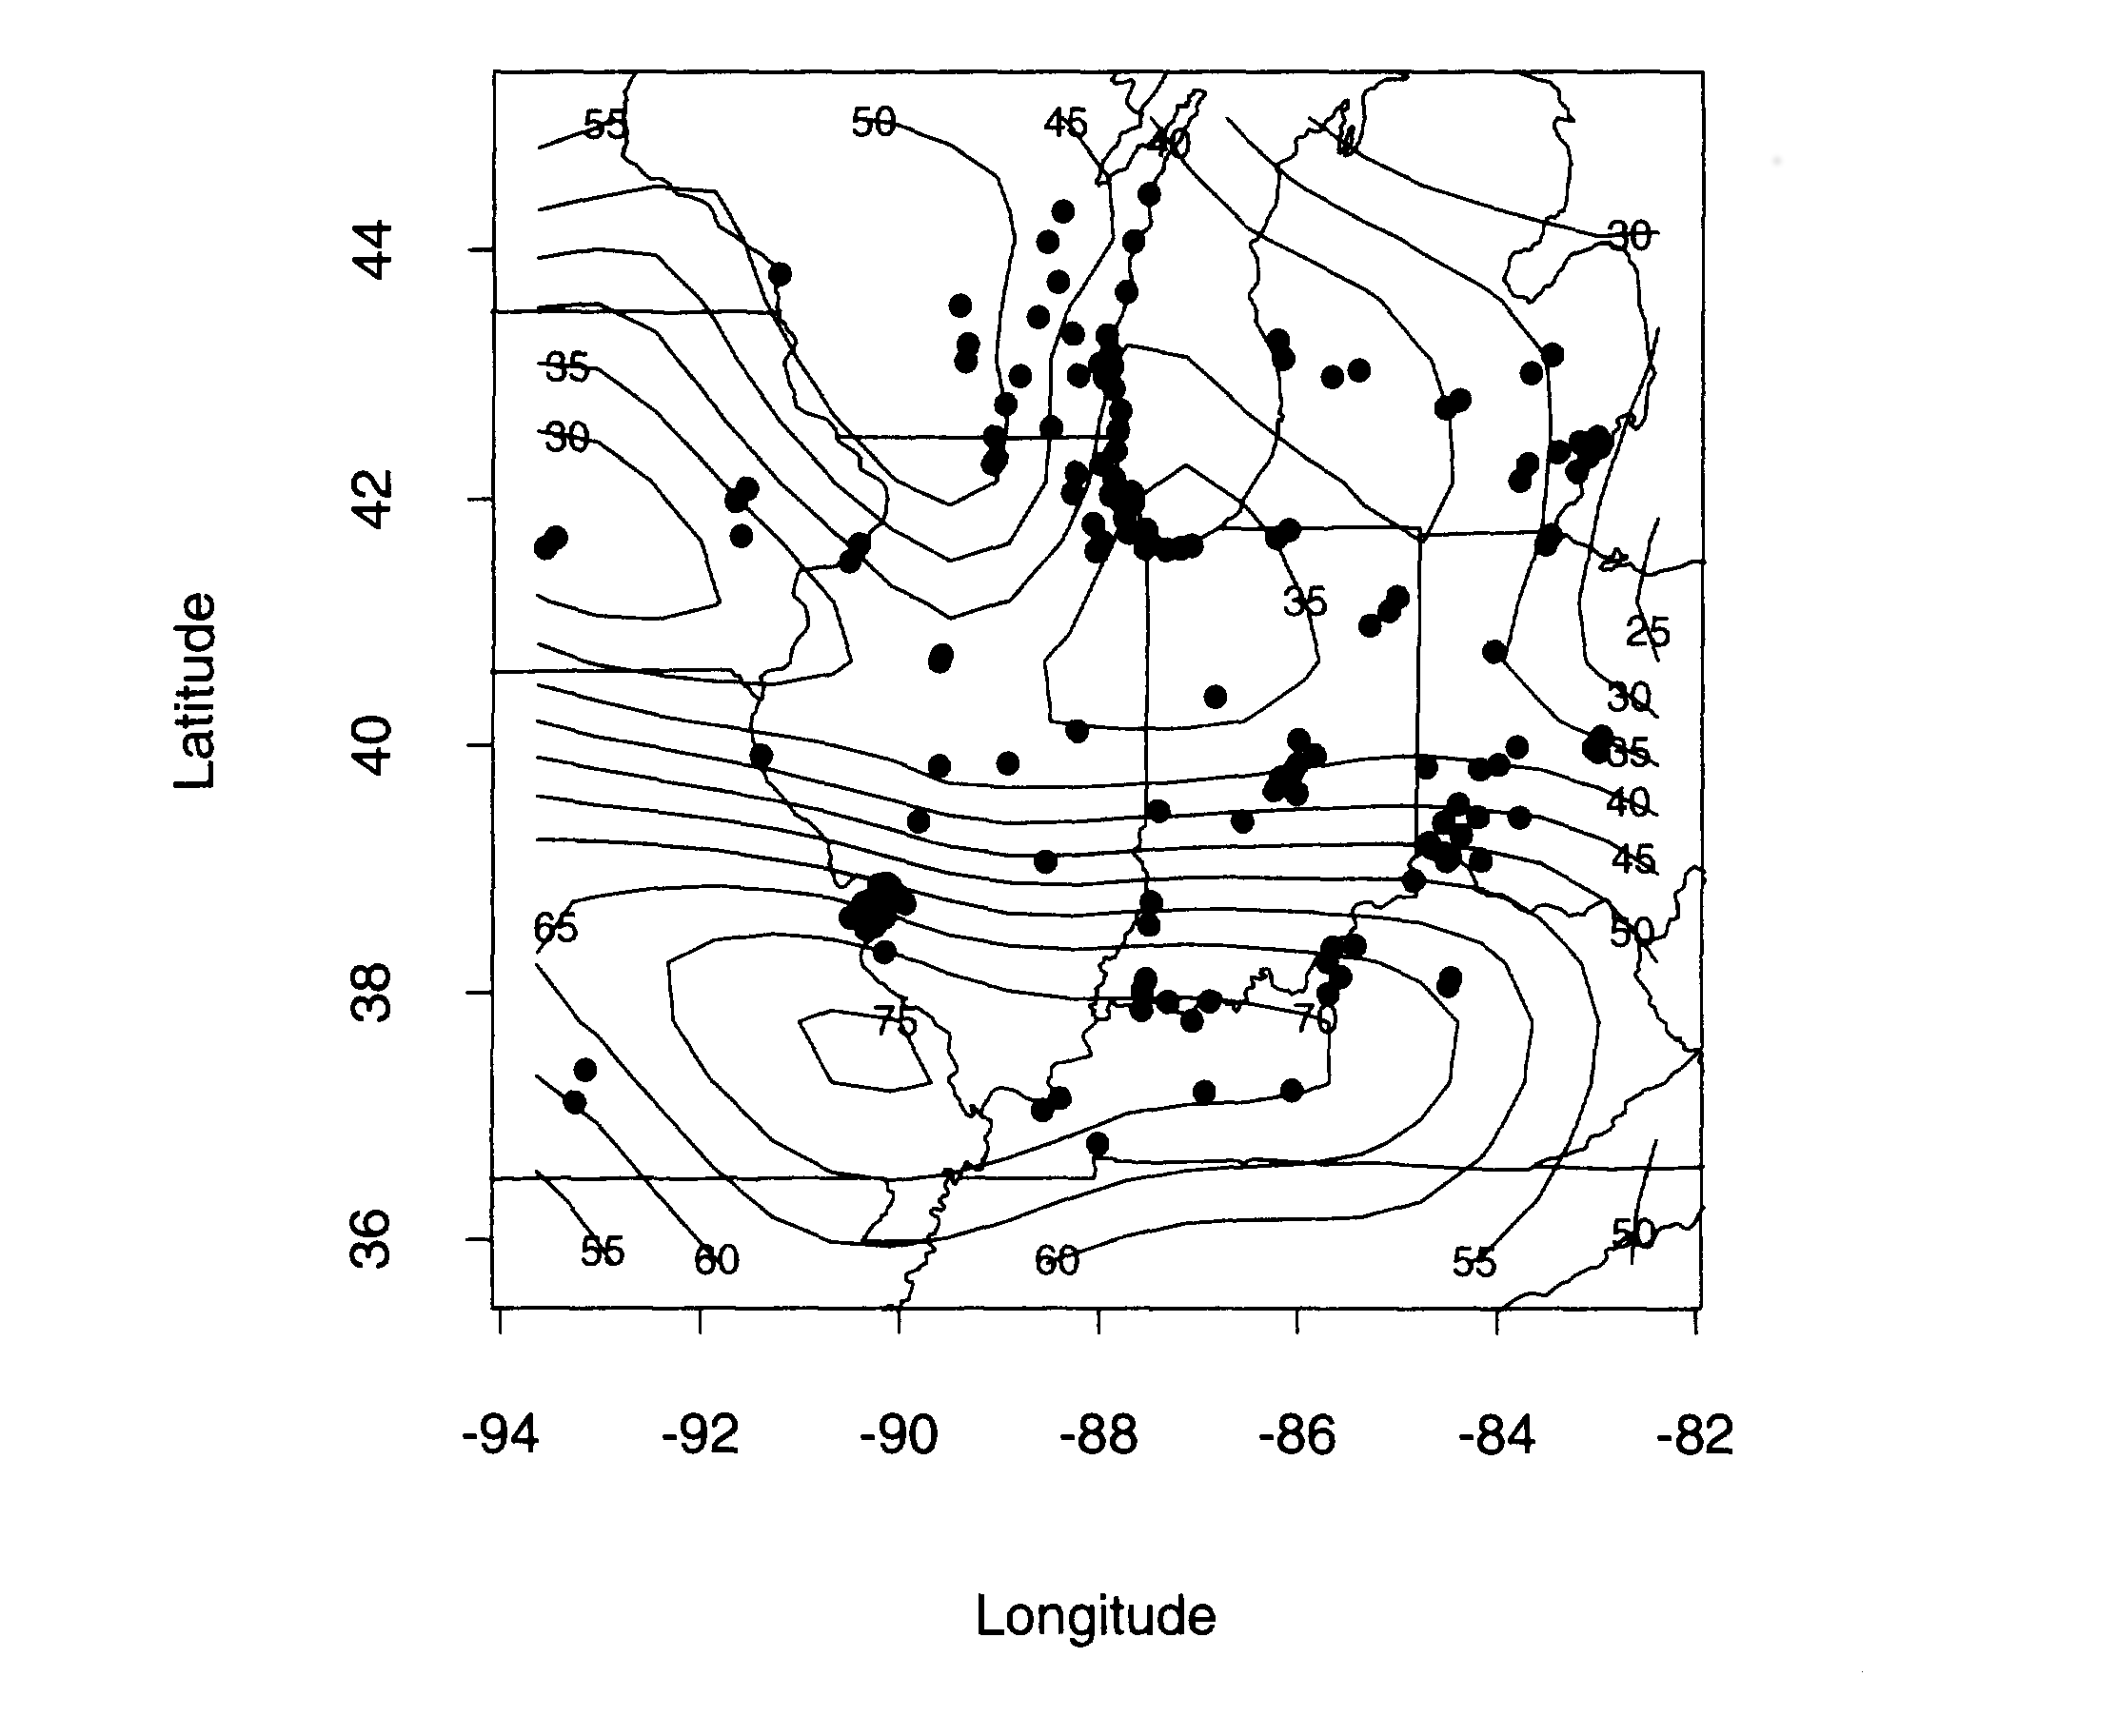
\includegraphics[width=2.5in]{./ozone.png}                                            
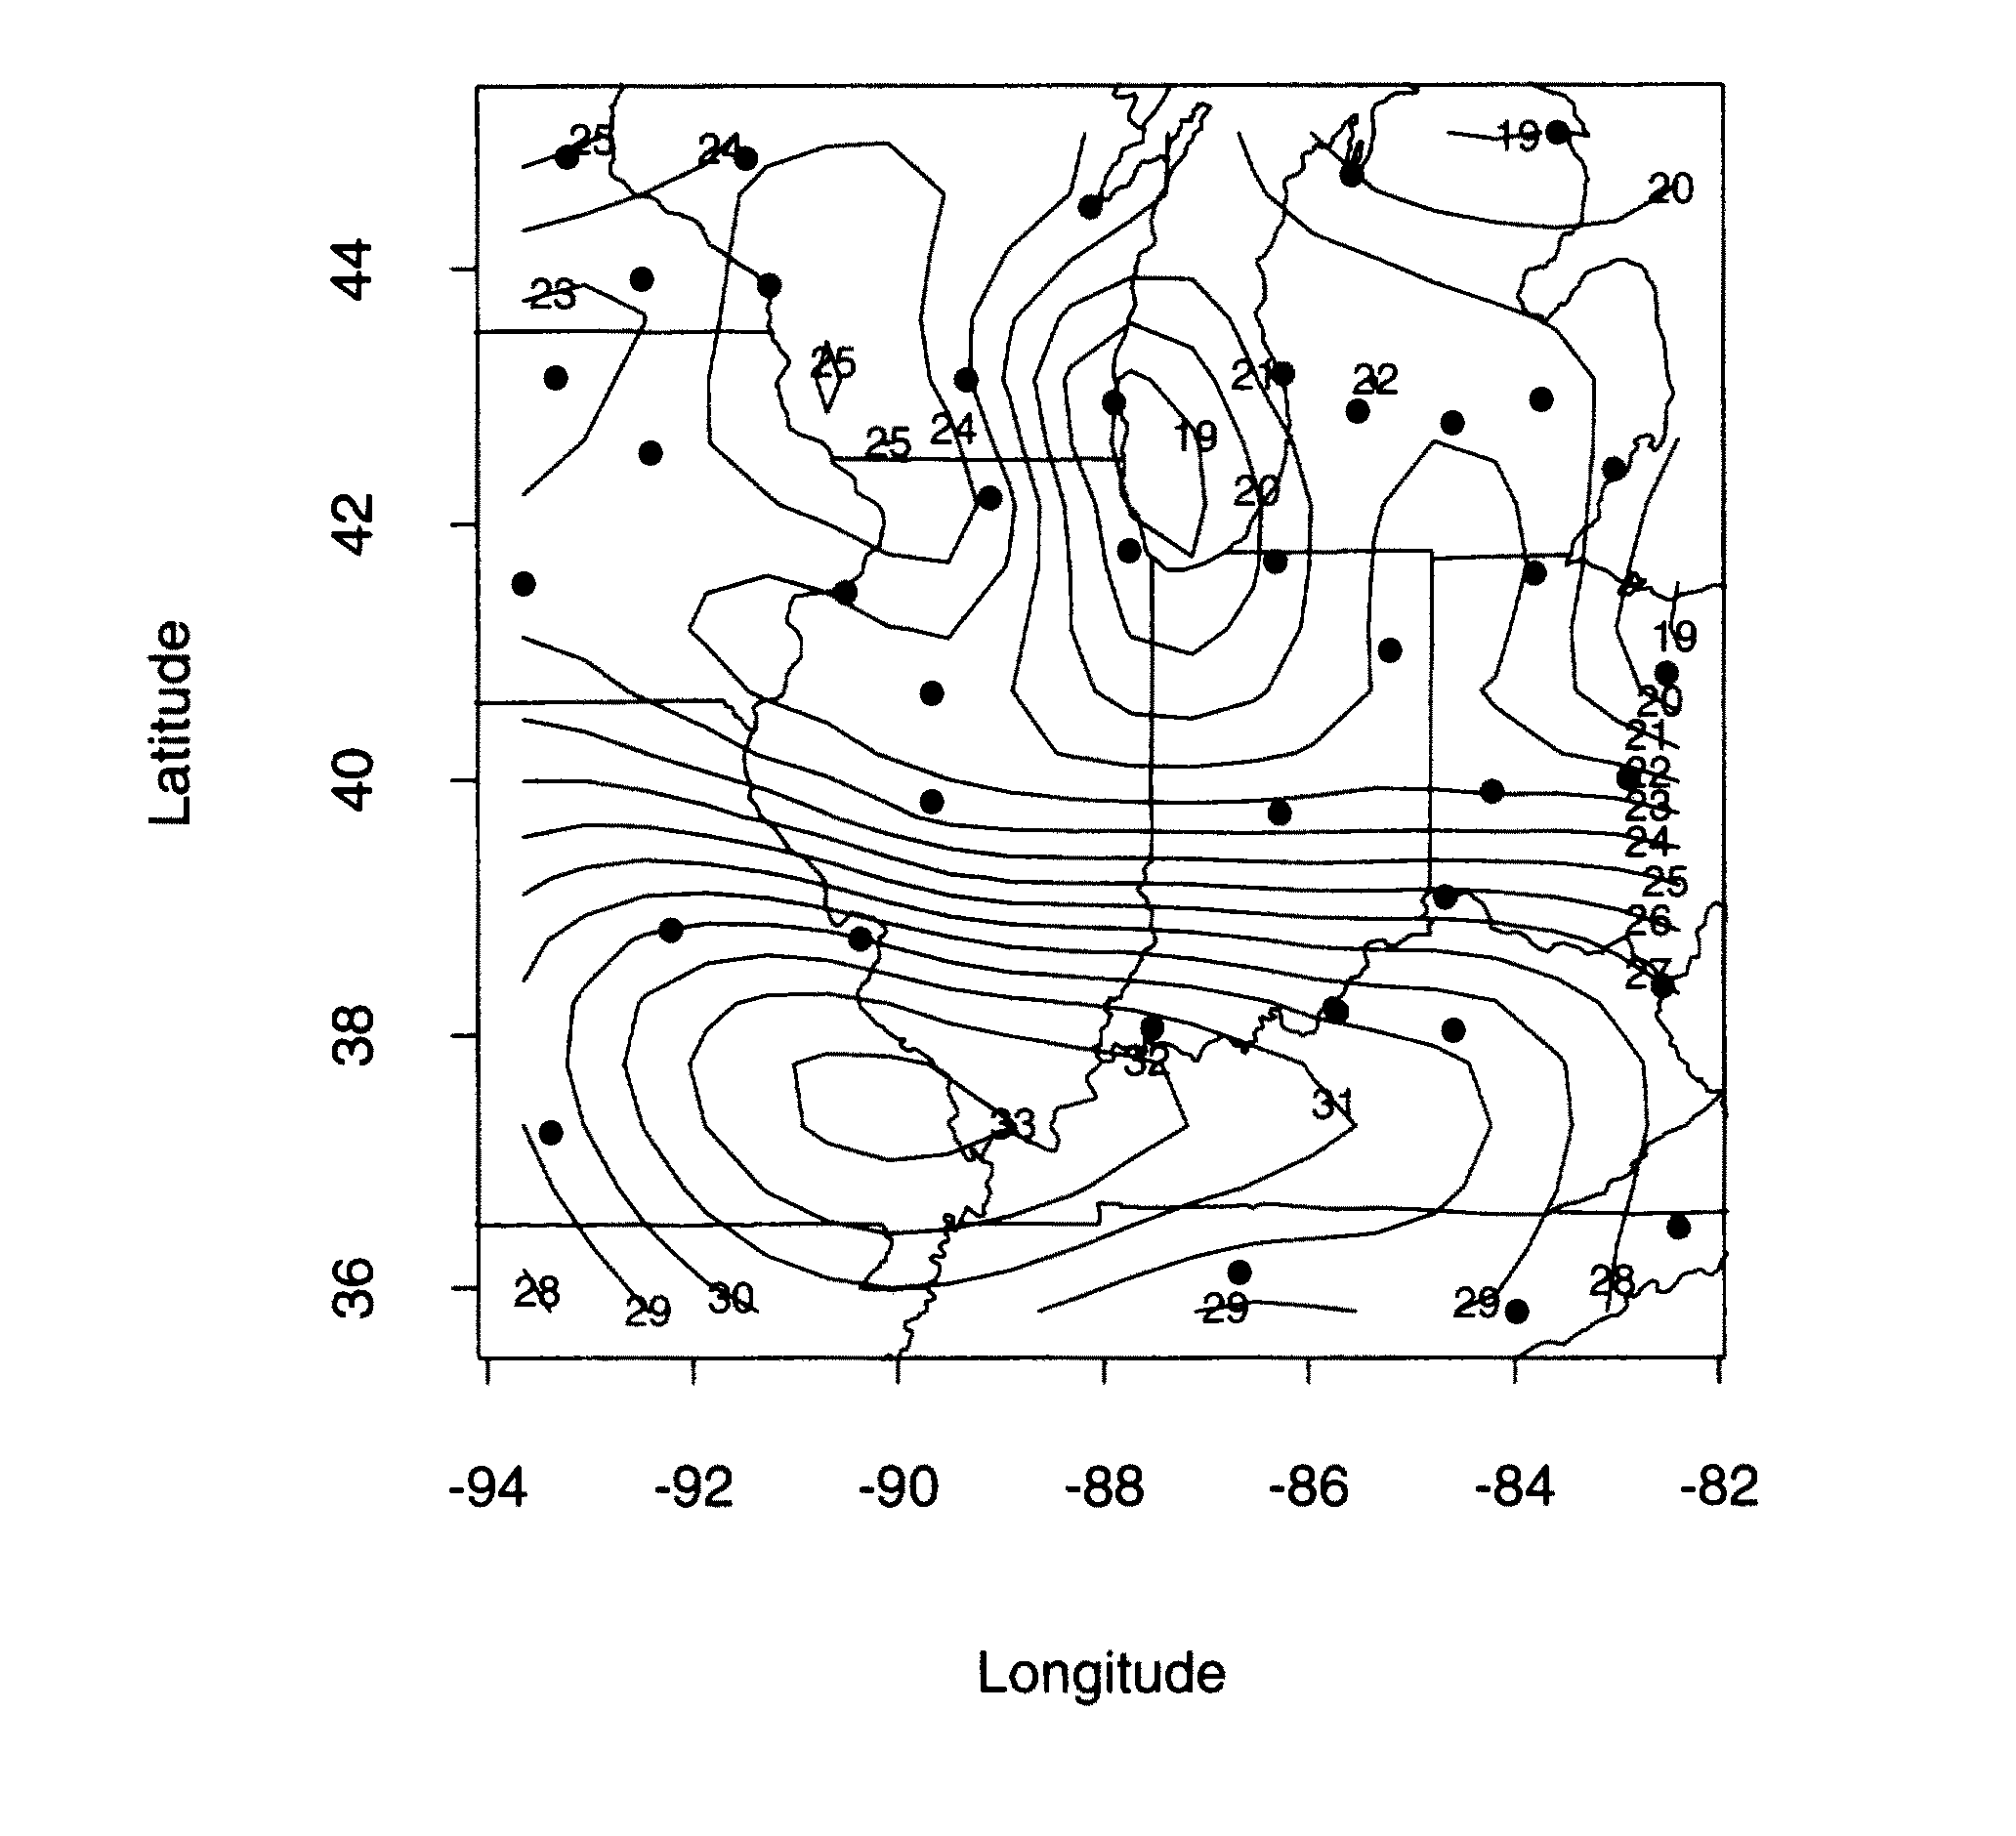
\includegraphics[width=2.3in]{./maxt.png}  
\end{center}
\end{frame}

% ###################

\begin{frame}
\frametitle{Example 2: Antarctica Mass Balance}

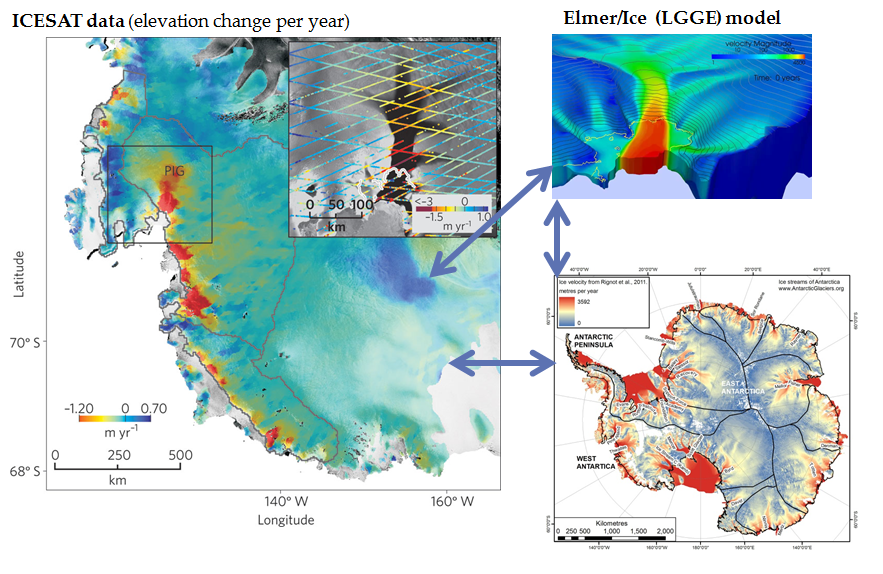
\includegraphics[width=4.5in]{./Antarctica.png}        
\end{frame}

% ###################

\begin{frame}
\frametitle{Example 2: Antarctica Mass Balance}

\begin{itemize}
\item \citet{Zammit_2014,Zammit_2015a,Zammit_2015b}, Antarctica.
\end{itemize}


\begin{center}
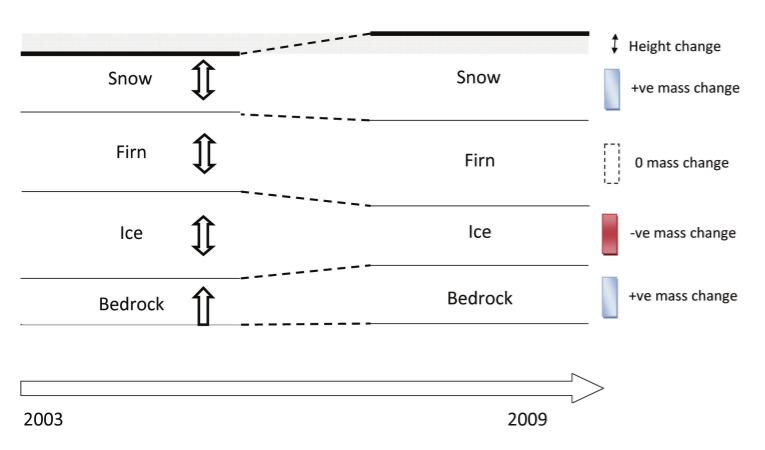
\includegraphics[width=4in]{./Obs.png}        
\end{center}

\end{frame}

% ###################

\begin{frame}
\frametitle{The challenge}

\begin{itemize}

\item {\bf Modelling}: Given a bivariate process $(Y_1(\cdot), Y_2(\cdot))$, what is a valid \emph{cross-covariance function matrix} (CCFM)
  
\begin{equation}
\left(\begin{array}{cc} C_{11}(\cdot,\cdot) & C_{12}(\cdot,\cdot) \\ C_{21}(\cdot,\cdot) & C_{22}(\cdot,\cdot)\end{array} \right),
\end{equation} 

such that {\bf any} covariance matrix derived from it is positive-definite? \vfill

\item {\bf Computational}: Sometimes we struggle with univariate models -- how do our algorithms scale to multivariate models? \vfill
\end{itemize}
\end{frame}

% ###################

\subsection{Current approaches}

\begin{frame}
\frametitle{Current approaches}

\begin{itemize}

\item {\bf Linear model of co-regionalisation} \citep[LMC,][]{Wackernagel1995}: Define
\begin{align}
    Y_1(\cdot) &= a_{11}\Yt_1(\cdot) + a_{12}\Yt_2(\cdot),\\
    Y_2(\cdot) &= a_{21}\Yt_1(\cdot) + a_{22}\Yt_2(\cdot),
\end{align}
where, independently,
\begin{align}
    \Yt_1(\cdot) &\sim \mathcal{N}(\mu_1(\cdot), C_{1}(\cdot,\cdot)),\\
    \Yt_2(\cdot) &\sim \mathcal{N}(\mu_2(\cdot), C_{2}(\cdot,\cdot)).
\end{align}

\item $C_{ij}(\cdot,\cdot) = a_{i1}a_{j1}C_{1}(\cdot,\cdot) + a_{i2}a_{j2}C_{2}(\cdot,\cdot)$.
\item CCFM is positive-definite for any $\{a_{ij}: i,j = 1,\dots,2\}$. 
\end{itemize}
\end{frame}

% ###################

\begin{frame}
\frametitle{Current approaches}

\begin{itemize}
\item {\bf Bivariate parsimonious Matérn model} \citep{Gneitingetal2010}: Let $C^o(\cdot)$ be a stationary, isotropic covariance function. Define
  
\begin{align}
    C_{ij}^o(\cdot) & \equiv \beta_{ij}M(\cdot; \nu_{ij}, \kappa_{ij}),
\end{align}

where $M(\cdot)$ is a Matérn covariance function. Let $\kappa_{ii} = \kappa_{ij} = \kappa$ and set $\nu_{ij} = (\nu_{ii} + \nu_{jj})/2$. Then if  $(\beta_{ij}:i,j = 1,2)$ is positive-definite, the CCFM is positive-definite.\vfill
  
\item {\bf Bivariate full Matérn model}:  Relaxes assumptions on smoothness and scales, but finding valid parameters is much more involved.\vfill
\end{itemize}

\end{frame}

% ###################

\begin{frame}
\frametitle{Current approaches (limitations)}

\begin{itemize}
\item Stuck with homogeneous models (e.g., convolution methods). \vfill
\item Stuck with fixed scales (parsimonious Matérn). \vfill
\item Stuck with Matérn models (e.g., full Matérn models). \vfill
\item {\bf Stuck with symmetry (e.g., LMC)}. \vfill
\end{itemize}

\end{frame}

% ###################

\begin{frame}
\frametitle{Asymmetry}

\begin{itemize}
\item $Y_1(\cdot)$: precipitation at present.        
\item $Y_2(\cdot)$: precipitation in 5 minutes time.
\end{itemize}

\begin{center}
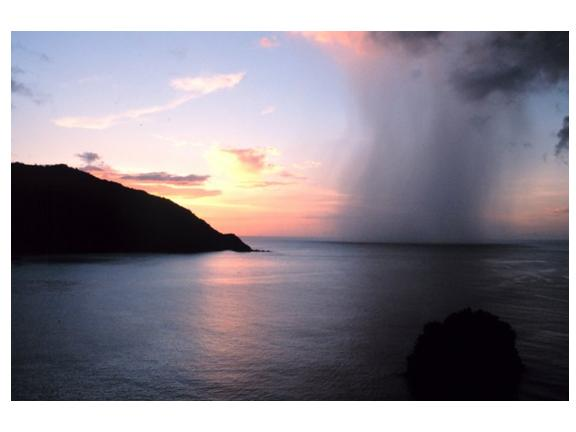
\includegraphics[width=3in]{rain.png}
\end{center}
\end{frame}

% ###################

\section{Causal spatial models}

\begin{frame}
\sectionpage
\end{frame}


\subsection{Bivariate models}

\begin{frame}
\frametitle{Causal spatial models}

Specification:
\begin{align}\label{eqn:E-and-cov}                                                          
\E\left(Y_2(\s)\mid Y_1(\cdot)\right)&\,=\int_D{b(\s,\v)Y_1(\v)\,\d \v};\quad \s\in D,\\
\cov\left(Y_2(\s),Y_2(\u)\mid Y_1(\cdot)\right)&\,=C_{2\mid 1}(\s,\u);\quad \s,\u\in \mathbb{R}^d.\end{align}  

Building blocks:
\begin{itemize}
\item $C_{11}(\cdot,\cdot)$,
\item $C_{2|1}(\cdot,\cdot)$,
\item $b(\cdot,\cdot)$ (interaction function).
\end{itemize}
\end{frame}

% ###################

\begin{frame}
\frametitle{Properties of causal spatial models}

\begin{itemize}
\item  CCFM is easy to find:

\begin{equation}
\begin{bmatrix} C_{11}(\s,\u) & \int_DC_{11}(\s,\v)b(\u,\v)\d\v \\ \int_Db(\s,\v)C_{11}(\v,\u)\d\v & ~~~~~C_{22}(\s,\u)\end{bmatrix};                     
\end{equation}

\begin{equation}
\small
C_{22}(\s,\u) = C_{2\mid 1}(\s,\u)+\int_D\int_D \red{b(\s,\v)} \blue{C_{11}(\v,\w)} \red{b(\w,\u)}\d\v\d\w,
\end{equation}

and is always valid (we will outline the proof soon). \vfill

\item Asymmetry (i.e., $C_{12}(\svec,\uvec) \ne C_{21}(\svec,\uvec)$) is guaranteed if $b(\cdot,\cdot)$ is not symmetric. \vfill
\end{itemize}
\end{frame}

% ###################

\begin{frame}
\frametitle{Properties of causal spatial models}

\begin{itemize}
\item Assume $b^o(\cdot) = b(\cdot,\cdot)$ and that it is off-centre.
\item $\s,\u \in \{-1, -0.9 ,\dots, 1\}$.
\end{itemize}

\begin{center}
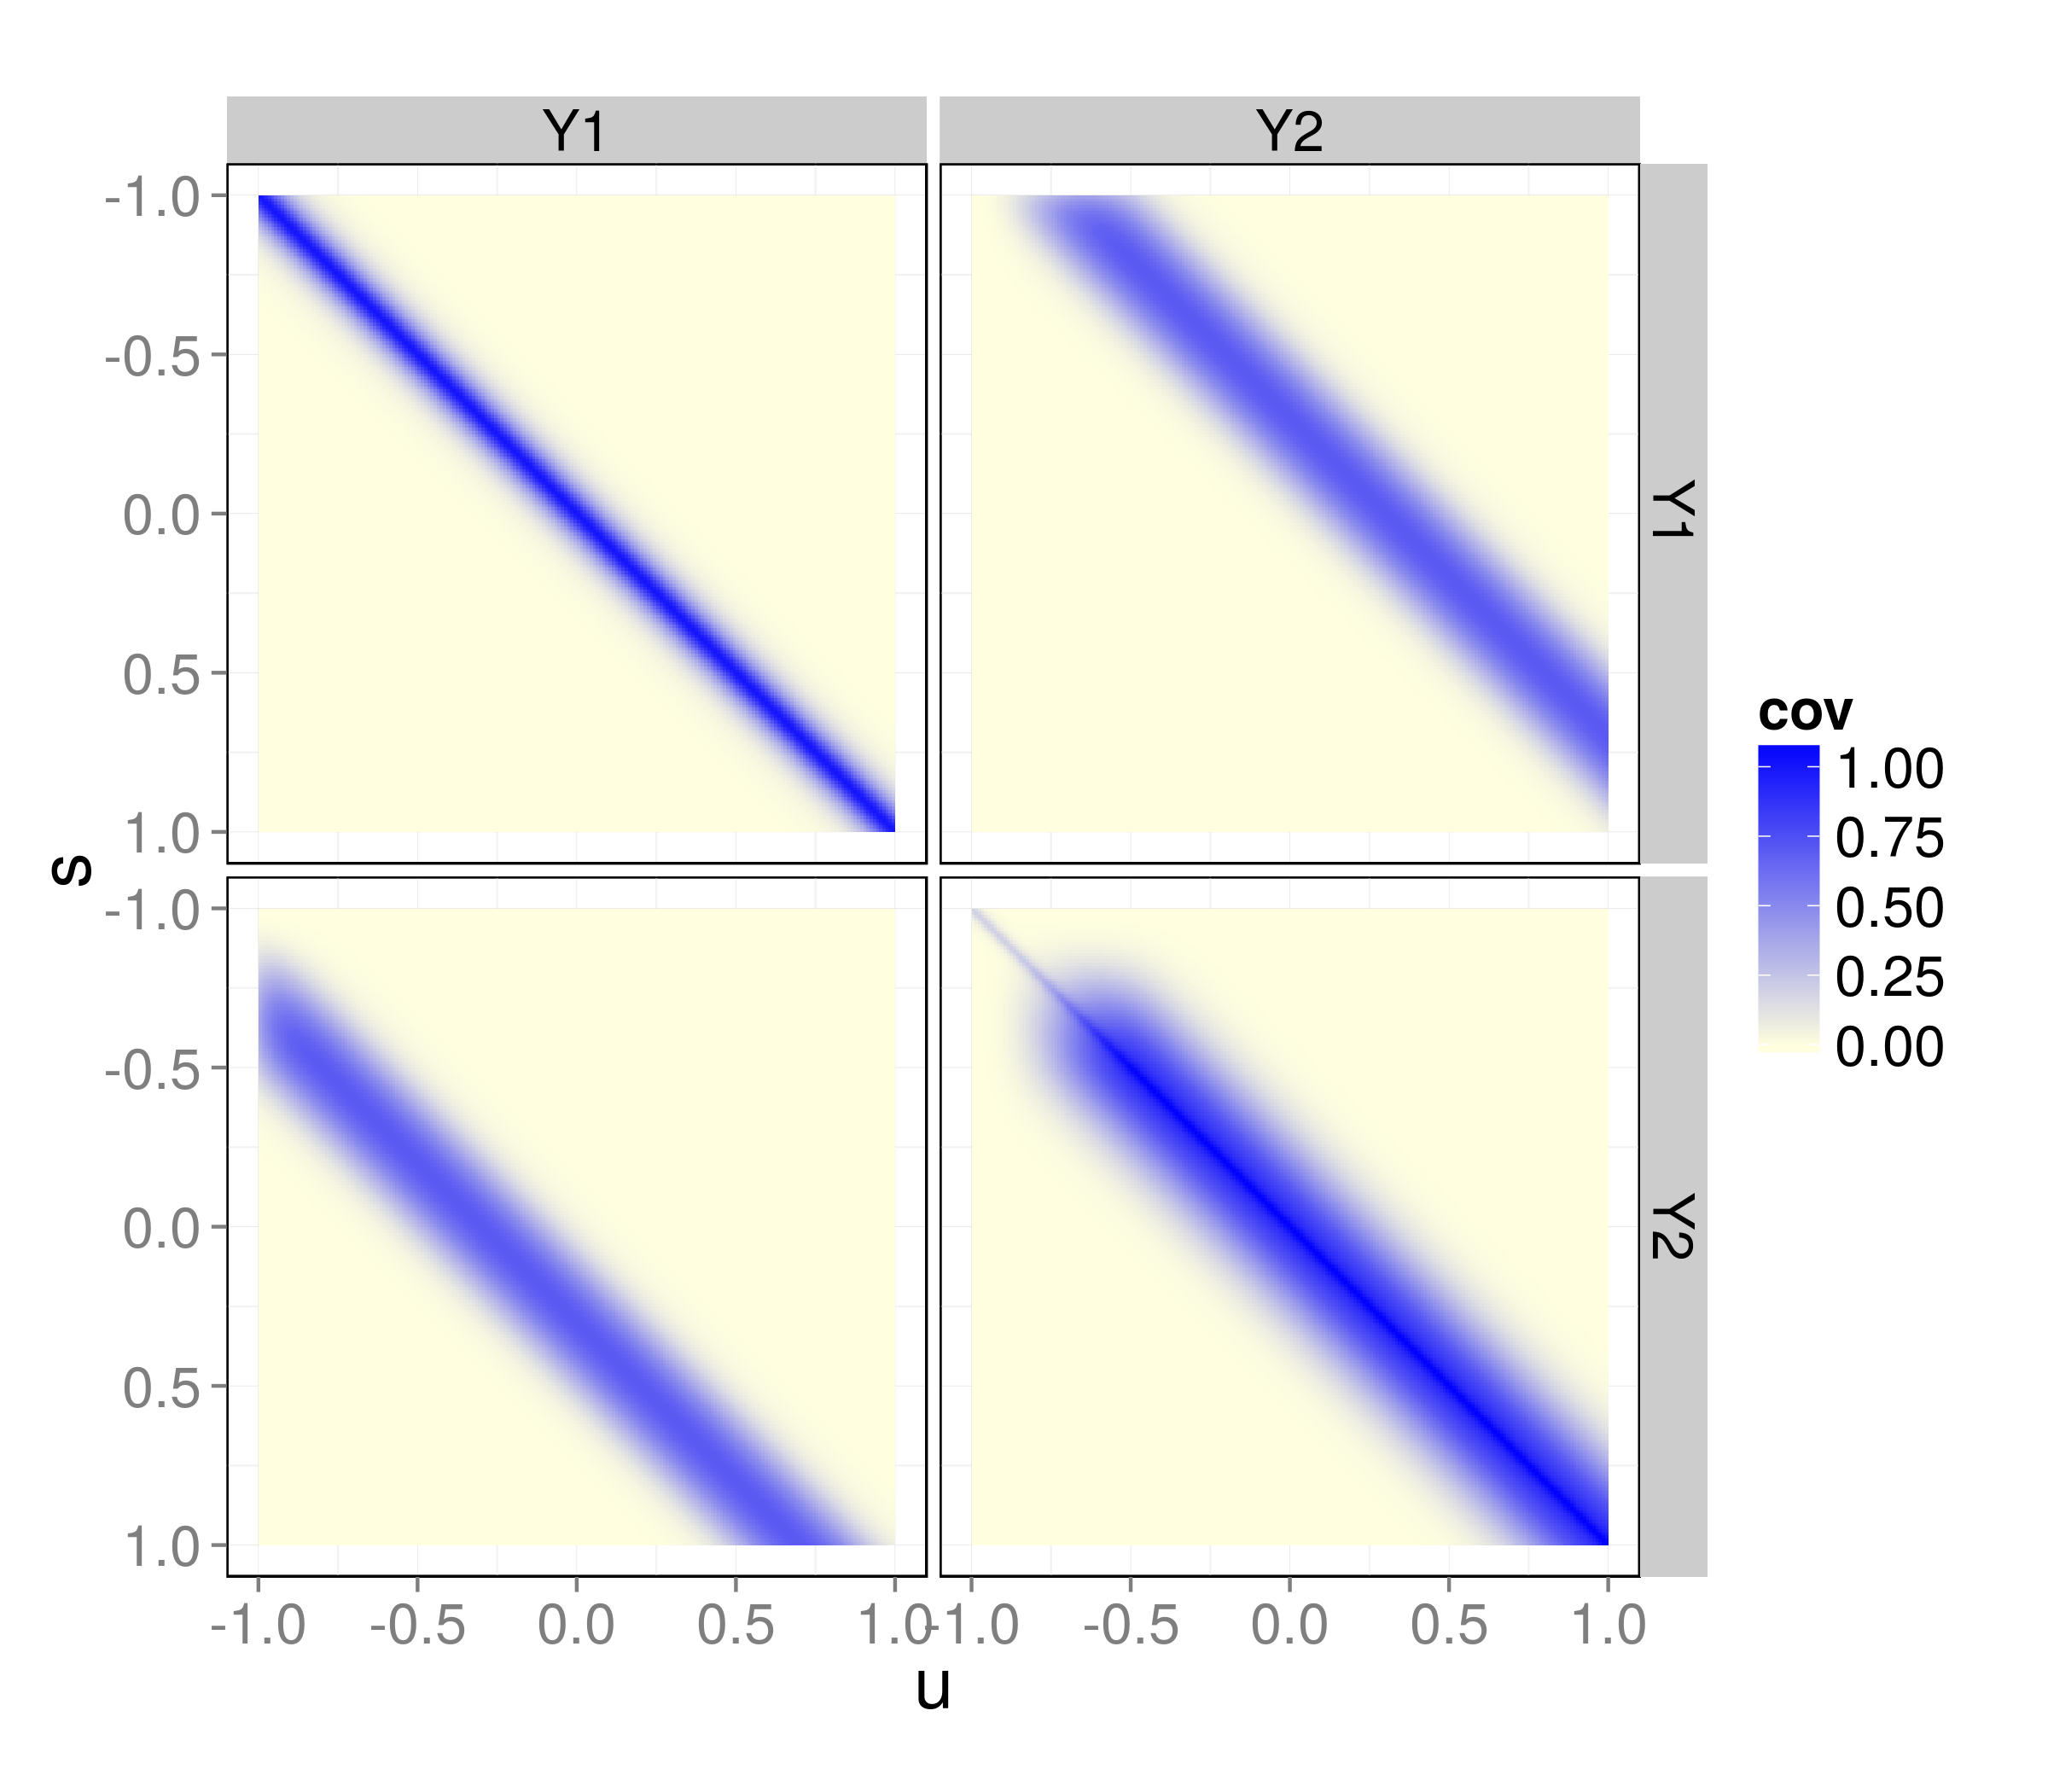
\includegraphics[width=2.5in]{Sigma.png}
\end{center}
\end{frame}

% ###################

\begin{frame}
\frametitle{Properties of causal spatial models}

\begin{itemize}
\item Heterogeneity, since $C_{11}(\cdot,\cdot)$, $C_{2|1}(\cdot,\cdot)$ need not be homogeneous and $b(\svec,\uvec)$ need not be symmetric. \vfill

\item We are not restricted to Matérn fields. The bivariate parsimonious Matérn field is a {\bf special case}.\vfill

\item $Y_2(\cdot)$ can be arbitrarily smoother than $Y_1(\cdot)$ {\bf and} have a different scale.\vfill

\end{itemize}
\end{frame}

% ###################

\begin{frame}
\frametitle{Example}

\begin{itemize}
\item Assume all parameters are known and $Y_1(\cdot)$ is only partially observed. \vfill
\item Use simple cokriging {\bf or} simple kriging to estimate $Y_1(\cdot)$:

\begin{align*}
\hat Y_1(\svec_0) &\equiv \E(Y_1(\svec_0) \mid  \Zvec_1, \Zvec_2)~~~~\textrm{simple cokriging predictor}, \\
\widetilde Y_1(\svec_0) &\equiv \E(Y_1(\svec_0) \mid  \Zvec_1)~~~~~~~~~\textrm{simple kriging predictor}.
\end{align*}\vfill
\end{itemize}

\end{frame}

% ###################

\begin{frame}
\frametitle{Example}
\begin{center}
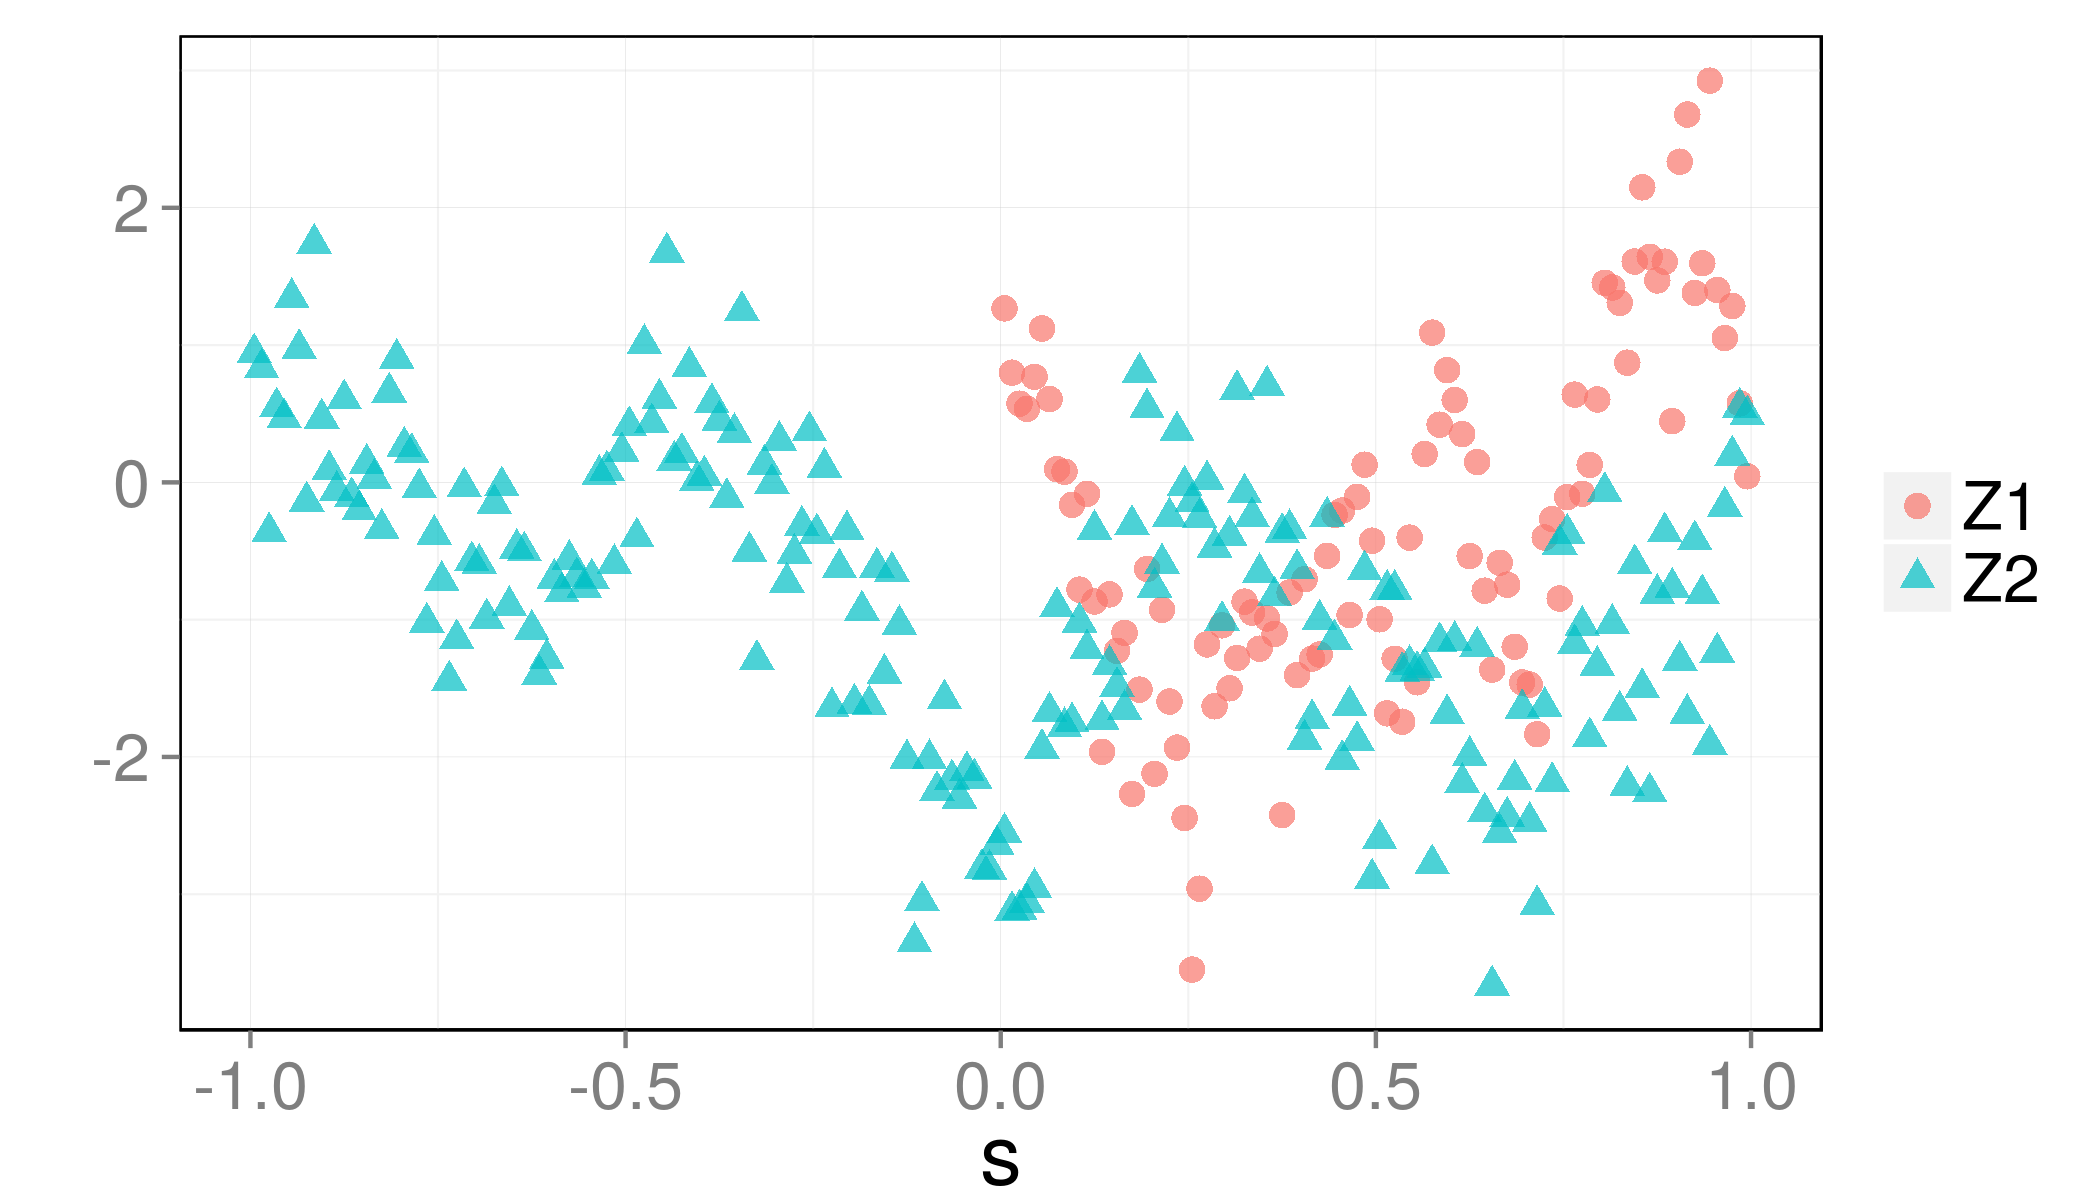
\includegraphics[width=4in]{./sim_obs.png}
\end{center}
\end{frame}

% ###################

\begin{frame}
\frametitle{Example}
\begin{center}
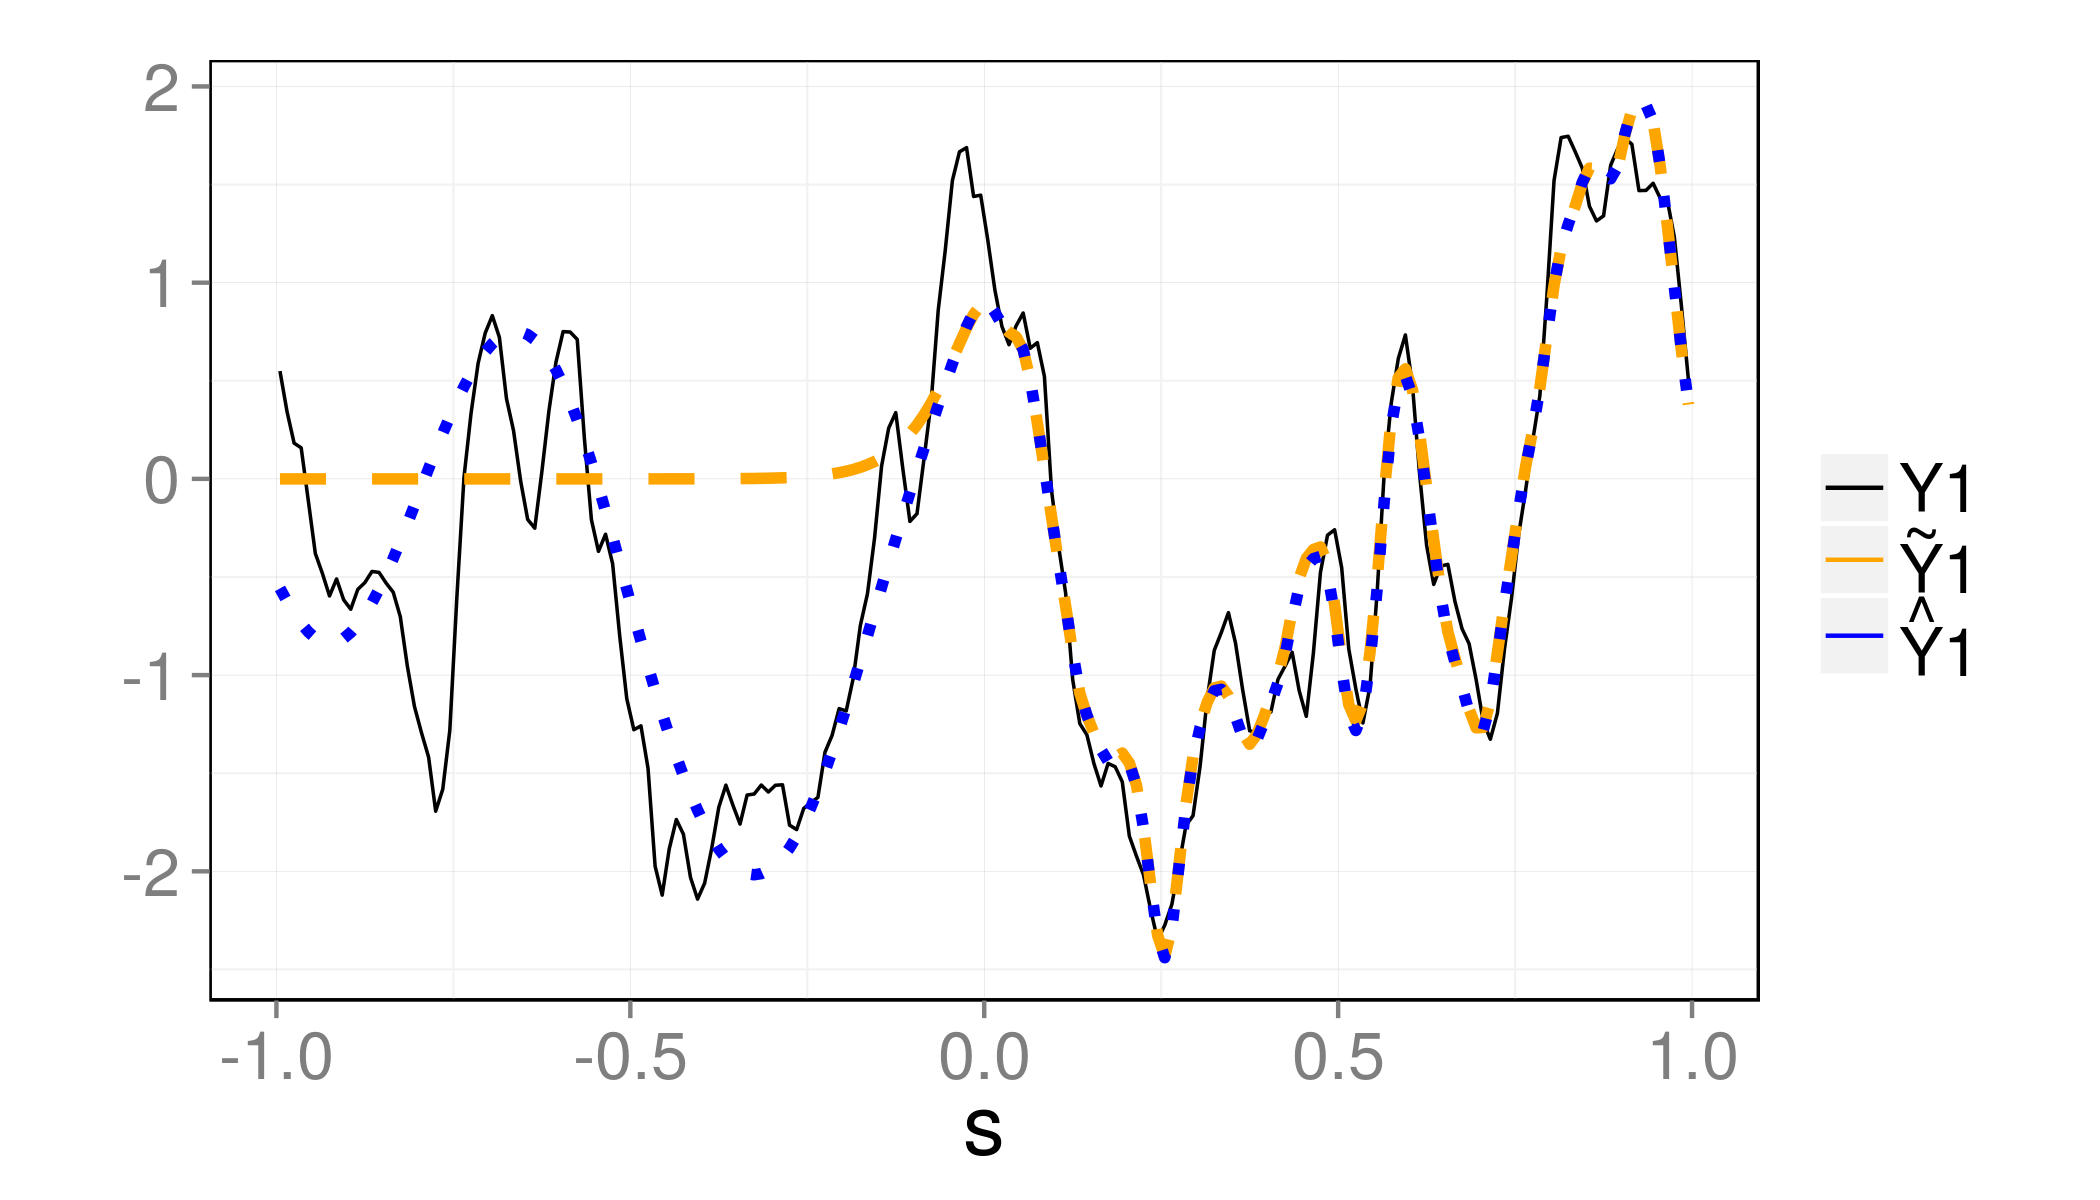
\includegraphics[width=4in]{./sim_est.png}
\end{center}
\end{frame}

% ###################

\begin{frame}
\frametitle{Is the bivariate model always valid?}

\begin{itemize}
\item If $C_{11}(\svec,\uvec)$ and $C_{2|1}(\svec,\uvec)$ are positive-definite, then $C_{22}(\cdot,\cdot)$ is positive-definite (recall quadratic form).
\item $C_{12}(\svec,\uvec) = C_{21}(\uvec,\svec)$.
\item CCFM is positive-definite if, for any $n_1,n_2$ such that $n_1 + n_2 > 0$, any locations $\{\svec_{1k}\}, \{\svec_{2l}\}$ and any real numbers $\{a_{1k}\},\{a_{2l}\}$,

\small
\begin{align*}
 & \var\left(\sum_{k=1}^{n_1}{a_{1k}Y_1^0(\s_{1k})}+\sum_{l=1}^{n_2}{a_{2l}Y_2^0(\s_{2l})}\right) \\ &=\sum_{k=1}^{n_1}\sum_{k'=1}^{n_1} a_{1k}a_{1k'}C_{11}^0(\s_{1k},\s_{1k'})+\sum_{l=1}^{n_2}\sum_{l'=1}^{n_2} a_{2l}a_{2l'}C_{22}^0(\s_{2l},\s_{2l'}) \\
  &+\sum_{k=1}^{n_1}\sum_{l'=1}^{n_2} a_{1k}a_{2l'}C_{12}^0(\s_{1k},\s_{2l'})+\sum_{l=1}^{n_2}\sum_{k'=1}^{n_1} a_{2l}a_{1k'}C_{21}^0(\s_{2l},\s_{1k'})~ \ge 0.
\end{align*}

\normalsize
\end{itemize}
\end{frame}

% ###################

\begin{frame}
\frametitle{Is the bivariate model always valid?}

\begin{itemize}
\item It can be shown that
\begin{align*}
& \var\left(\sum_{k=1}^{n_1}{a_{1k}Y_1^0(\s_{1k})}+\sum_{l=1}^{n_2}{a_{2l}Y_2^0(\s_{2l})}\right)\\
&= \sum_{l=1}^{n_2}\sum_{l'=1}^{n_2}a_{2l}a_{2l'}C_{2\mid 1}(\s_{2l},\s_{2l'})+\int_D \int_D{\red{a(\s)a(\u)}\blue{C_{11}(\s,\u)}\,\d\s\d\u},
\end{align*}
where

\begin{equation*}
a(\s)\equiv \sum_{k=1}^{n_1}a_{1k}\delta(\s-\s_{1k})+\sum_{l=1}^{n_2}a_{2l}b(\s_{2l},\s);\quad \s\in \RR^d.
\end{equation*}

\end{itemize}
\end{frame}

% ###################

\subsection{Multivariate models}

\begin{frame}
\frametitle{Beyond two dimensions}

\begin{itemize}
\item  $[Y_1(\cdot),\dots,Y_p(\cdot)]$ can be decomposed as,

\begin{equation*}
[Y_p(\cdot) \mid  Y_{p-1}(\cdot),Y_{p-2}(\cdot),\dots,Y_1(\cdot)]\dots [Y_1(\cdot)].                  \end{equation*} \pause

\item The conditional expectation is
\begin{align*}
\E(Y_q(\svec) \mid  \{Y_r(\cdot) : r = 1,\dots,(q-1)\}) \equiv \sum_{r = 1}^{q-1} \int_D b_{qr}(\svec,\v)Y_r(\v) \intd \v; \\
 \qquad \qquad \svec \in D.
\end{align*} \pause

\item The conditional covariance is
\begin{align*}
\cov(Y_q(\svec), Y_q(\uvec) \mid  \{Y_r(\cdot) : r = 1,\dots,(q-1)\}) \equiv C_{q \mid  (r < q)}(\svec,\uvec);\\  \qquad\qquad \svec,\uvec \in \mathbb{R}^d,
\end{align*}
where $\{b_{qr}(\cdot,\cdot) : r = 1,\dots,(q-1) ;~q = 2,\dots,p\}$ are integrable.

\end{itemize}
\end{frame}

% ###################

\begin{frame}
\frametitle{Is the multivariate model always valid?}

We need to show that the $p$-variate process is well defined. The proof is by induction:
\begin{itemize}
  \item We know that the bivariate process is well defined.
  \item Assume that the $(p-1)$-variate process is well defined.
  \item Show that the $p$-variate process is well defined.
\end{itemize}

\vspace{-0.3in}
\begin{align*}
\var\left(\sum_{q=1}^p \sum_{m=1}^{n_q} a_{qm}Y_q(\svec_{qk})\right)=& \sum_{m=1}^{n_p}\sum_{m'=1}^{n_p}a_{pm}a_{pm'}C_{p \mid  (q < p)}(\svec_{pm},\svec_{pm'}) \\
&+ \sum_{q=1}^{p-1}\sum_{r=1}^{p-1}\int_D\int_D\red{a_q(\svec)a_r(\uvec)}\blue{C_{qr}(\svec,\uvec)}\intd \svec \intd \uvec, 
\end{align*}
where
\begin{equation*}
a_q(\svec) \equiv \left(\sum_{k=1}^{n_q}a_{qk}\delta(\svec - \svec_{qk}) + \sum_{m=1}^{n_p}a_{pm}b_{pq}(\svec_{pm},\svec)\right).
\end{equation*}
\end{frame}

% ###################

\begin{frame}
\frametitle{Generalisations}

The following can all be shown to be special cases of causal spatial models:

\begin{itemize}
\item The parsimonious Mat{\'e}rn model of \cite{Gneitingetal2010},
\item The full Mat{\'e}rn model of \cite{Gneitingetal2010},
\item The linear model of coregionalisation, used for example by \cite{Wackernagel1995},
\item The moving average model of \cite{verHoef_1998}.
\end{itemize}
\end{frame}

% ###################

\begin{frame}
\frametitle{Graphical structure}

\begin{itemize}
\item No restriction on graphical structure. It could be undirected, directed, or a chain graph \citep{Lauritzen_1996}.
\item Computationally-efficient algorithms available for some structures.
\end{itemize}

\begin{figure}[!t]
\begin{center}

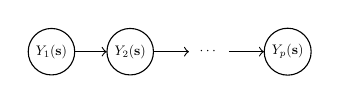
\begin{tikzpicture}[scale=0.5,every node/.style={transform shape}]
%[inner sep=1mm] 
[line width=1pt]

\path (0,0) node (Y1) [shape=circle, minimum size=1cm,draw] {$Y_1(\svec)$};
\path (2,0) node (Y2) [shape=circle, minimum size=1cm,draw] {$Y_2(\svec)$};
\path (4,0) node (dots) [shape=circle, minimum size=1cm] {$\cdots$};
\path (6,0) node (Yp)  [shape=circle, minimum size=1cm,draw] {$Y_p(\svec)$};

\draw [->] (Y1) to (Y2);
\draw [->] (Y2) to (dots);
\draw [->] (dots) to (Yp);

\end{tikzpicture}
\caption{Ordered nodes}\label{fig:exchangeable}
\end{center}
\end{figure}

\begin{figure}[!t]
\begin{center}

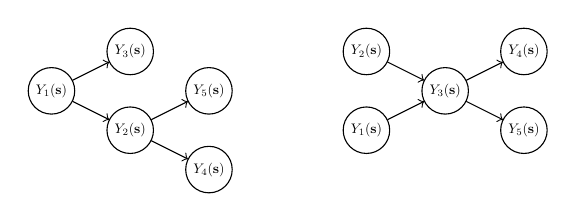
\begin{tikzpicture}[scale=0.5,every node/.style={transform shape}]
%[inner sep=1mm] 
[line width=1pt]

\path (0,0) node (Y1) [shape=circle, minimum size=1cm,draw] {$Y_1(\svec)$};
\path (2,-1) node (Y3) [shape=circle, minimum size=1cm,draw] {$Y_2(\svec)$};
\path (2,1) node (Y2) [shape=circle, minimum size=1cm,draw] {$Y_3(\svec)$};
\path (4,-2) node (Y4)  [shape=circle, minimum size=1cm,draw] {$Y_4(\svec)$};
\path (4,0) node (Y5)  [shape=circle, minimum size=1cm,draw] {$Y_5(\svec)$};

\draw [->] (Y1) to (Y2);
\draw [->] (Y1) to (Y3);
\draw [->] (Y3) to (Y4);
\draw [->] (Y3) to (Y5);


\path (8,-1) node (Y1b) [shape=circle, minimum size=1cm,draw] {$Y_1(\svec)$};
\path (8,1) node (Y2b) [shape=circle, minimum size=1cm,draw] {$Y_2(\svec)$};
\path (10,0) node (Y3b) [shape=circle, minimum size=1cm,draw] {$Y_3(\svec)$};
\path (12,1) node (Y4b)  [shape=circle, minimum size=1cm,draw] {$Y_4(\svec)$};
\path (12,-1) node (Y5b)  [shape=circle, minimum size=1cm,draw] {$Y_5(\svec)$};

\draw [->] (Y1b) to (Y3b);
\draw [->] (Y2b) to (Y3b);
\draw [->] (Y3b) to (Y4b);
\draw [->] (Y3b) to (Y5b);


\end{tikzpicture}

\caption{Trees and polytrees}
\end{center}

\end{figure}

\end{frame}

% ###################

\begin{frame}
\frametitle{Model flexibility}

\begin{figure}[!t]
\begin{center}

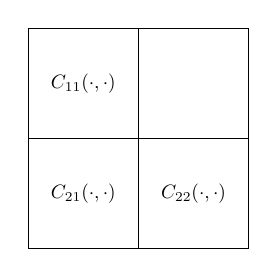
\begin{tikzpicture}[scale=0.7,every node/.style={transform shape}]
%[inner sep=1mm] 
[line width=1pt]

\path (0,0) node (X11) [shape=rectangle, minimum size=2cm,draw] {$C_{11}(\cdot,\cdot)$};
\path (2,0) node (X12) [shape=rectangle, minimum size=2cm,draw] {};
\path (0,-2) node (X21) [shape=rectangle, minimum size=2cm,draw] {$C_{21}(\cdot,\cdot)$};
\path (2,-2) node (X22)  [shape=rectangle, minimum size=2cm,draw] {$C_{22}(\cdot,\cdot)$};


\end{tikzpicture}
\caption{Bivariate system: Need to specify three marginal/cross-covariance functions.}\label{fig:exchangeable}
\end{center}
\end{figure}

Available building blocks: Three functions, $C_{11}(\cdot,\cdot)$, $C_{2\mid 1}(\cdot,\cdot)$, $b(\cdot,\cdot)$.

\end{frame}

% ###################

\begin{frame}
\frametitle{Model flexibility}

\begin{figure}[!t]
\begin{center}

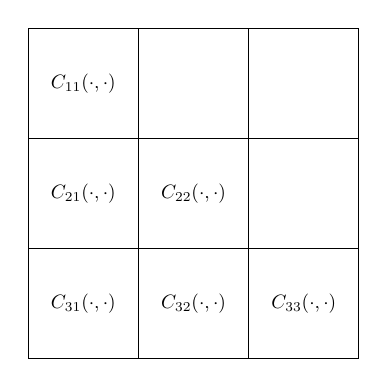
\begin{tikzpicture}[scale=0.7,every node/.style={transform shape}]
%[inner sep=1mm] 
[line width=1pt]

\path (0,0) node (X11) [shape=rectangle, minimum size=2cm,draw] {$C_{11}(\cdot,\cdot)$};
\path (2,0) node (X12) [shape=rectangle, minimum size=2cm,draw] {};
\path (4,0) node (X13) [shape=rectangle, minimum size=2cm,draw] {};
\path (0,-2) node (X21) [shape=rectangle, minimum size=2cm,draw] {$C_{21}(\cdot,\cdot)$};
\path (2,-2) node (X22)  [shape=rectangle, minimum size=2cm,draw] {$C_{22}(\cdot,\cdot)$};
\path (4,-2) node (X23)  [shape=rectangle, minimum size=2cm,draw] {};
\path (0,-4) node (X31) [shape=rectangle, minimum size=2cm,draw] {$C_{31}(\cdot,\cdot)$};
\path (2,-4) node (X32)  [shape=rectangle, minimum size=2cm,draw] {$C_{32}(\cdot,\cdot)$};
\path (4,-4) node (X33)  [shape=rectangle, minimum size=2cm,draw] {$C_{33}(\cdot,\cdot)$};


\end{tikzpicture}
\caption{Trivariate system: Need to specify six marginal/cross-covariance functions.}\label{fig:exchangeable}
\end{center}
\end{figure}

\vspace{-0.3cm}
Available building blocks: Six functions, $C_{11}(\cdot,\cdot)$, $C_{2\mid 1}(\cdot,\cdot)$, $C_{3|1,2}(\cdot,\cdot)$, $b_{21}(\cdot,\cdot)$, $b_{31}(\cdot,\cdot)$, $b_{32}(\cdot,\cdot)$.

\end{frame}

% ###################

\subsection{Min-max temperature dataset}

\begin{frame}
\frametitle{Min-max temperatures in Colorado, USA}

\begin{itemize}
\item Minimum and maximum temperatures taken on September 19, 2004 in the state of Colorado, USA.
\item 94 measurement stations (collocated measurements); residuals are obtained by subtraction of statewide mean.
\item Maximum-temperature residual later in the afternoon ($Y_2(\cdot)$) highly dependent on minimum-temperature residual in the early morning hours ($Y_1(\cdot)$).
\item Fit three models and compare using DIC:

\begin{equation*}
\begin{array}{ll}
\textrm{Model 1:} &b_o(\h) \equiv 0, \\
\textrm{Model 2:} &b_o(\h) \equiv A\delta(\h), \\
\textrm{Model 3:} &b_o(\h) \equiv \left\{\begin{array}{ll} A\{1 - (\|\h - \Deltab\|/r)^2\}^2, & \| \h - \Deltab\| \le r \\ 0, & \textrm{otherwise}. \end{array} \right. 
\end{array}
\end{equation*}
\end{itemize}
\end{frame}

% ###################

\begin{frame}
\frametitle{Discretisations}
\begin{itemize}
\item Consider a discretisation of $Y_1(\cdot)$ and $Y_2(\cdot)$, $\Yvec_1$ and $\Yvec_2$ respectively, and let $\Yvec \equiv (\Yvec_1,\Yvec_2)'$, $\Zvec \equiv (\Zvec_1,\Zvec_2)'$.
\end{itemize}

\vspace{-0.1in}
\begin{center}
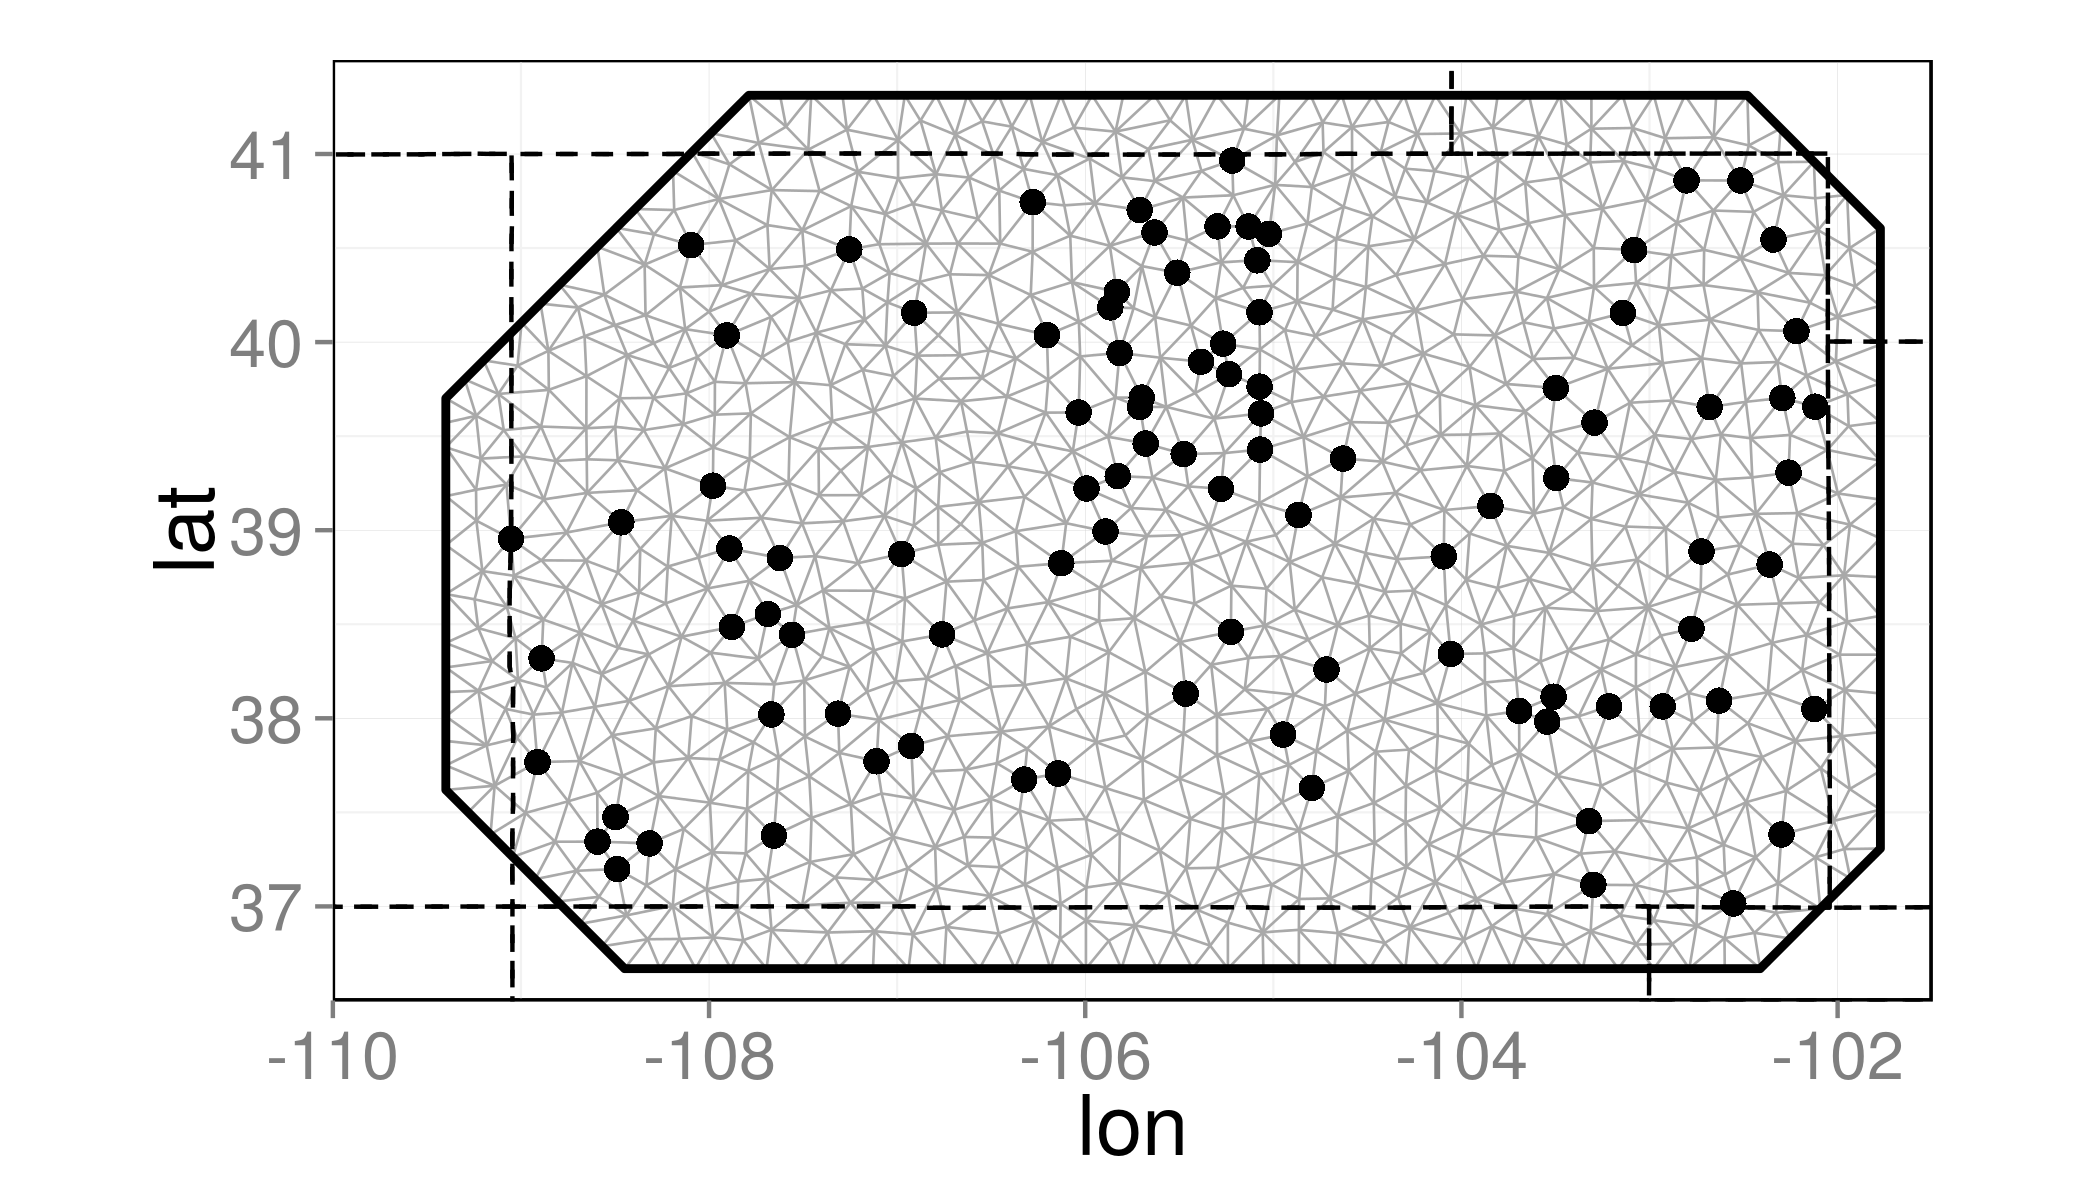
\includegraphics[width=4in]{meshplot.png}
\end{center}

\end{frame}

% ###################

 \begin{frame}
 \frametitle{Why use finite elements?}

 \begin{center}
 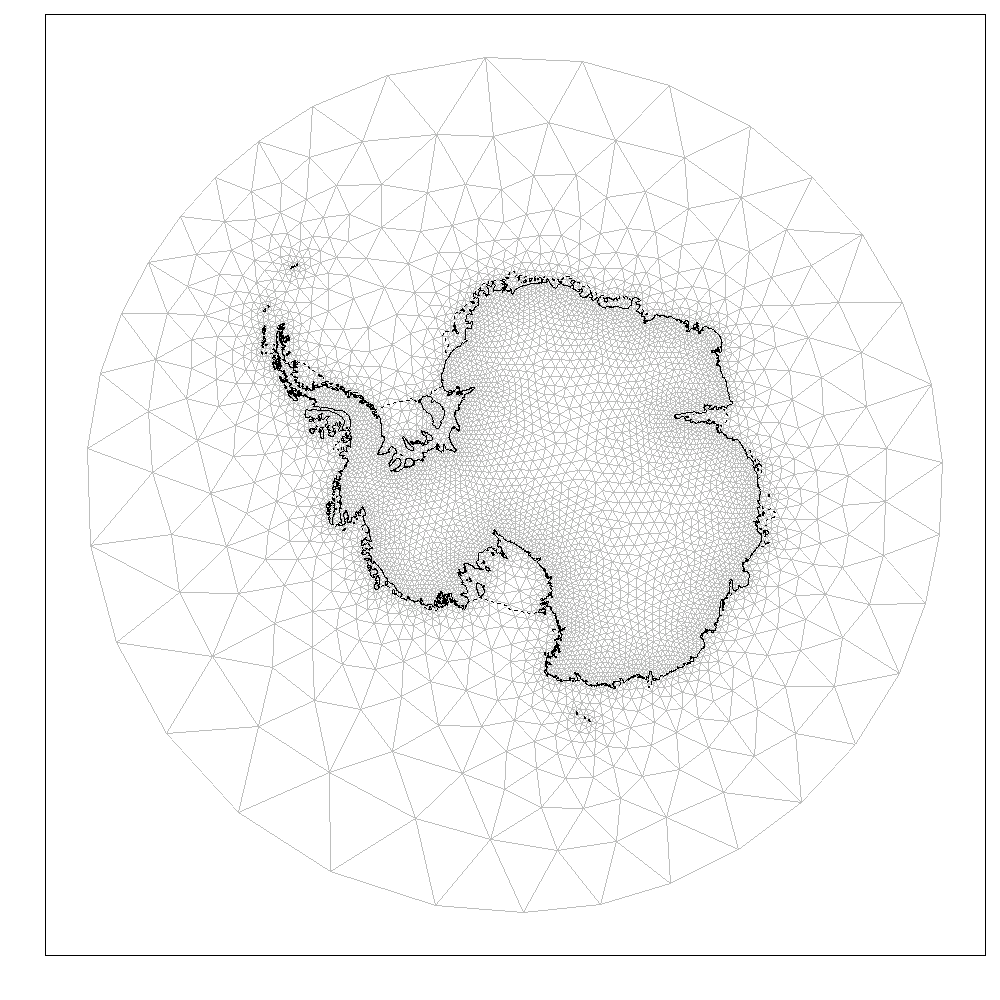
\includegraphics[width=3in]{ice_mesh.png}
 \end{center}

 \end{frame}

% ###################

\begin{frame}
\frametitle{Numerical integrations}

\vspace{-1cm}

\begin{center}
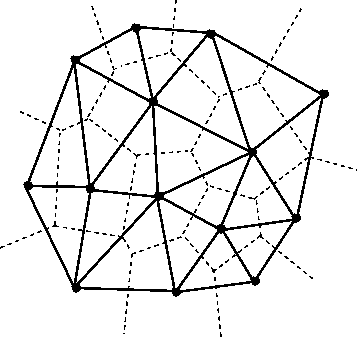
\includegraphics[width=2in]{vor3.png}
\end{center}

\vspace{-1.5cm}

\begin{align*}
\E\left(Y_2(\s)\mid Y_1(\cdot)\right)&=\int_D{b(\s,\v)Y_1(\v)\,\d \v};\quad \s\in D.\\
\E(Y_2(\svec_l) \mid  Y_1(\cdot)) &\simeq \sum_{k=1}^{n} \eta_k b(\svec_l,\v_k)Y_1(\v_k),
\end{align*}
where $\{\eta_k\}$ are the tessellation areas.
\end{frame}

% ###################

\begin{frame}
\frametitle{Full model}

\begin{itemize}
\item Observation model:
\begin{align*}
\left.\begin{pmatrix} \Zvec_1 \\ \Zvec_2 \end{pmatrix}
\right|
\begin{pmatrix} \Yvec_1 \\ \Yvec_2 \end{pmatrix} \hspace{-0.02in} ,\thetab
\sim
\mathcal{N}\left(
\begin{pmatrix} \Dmat\Yvec_1 \\ \Dmat\Yvec_2 \end{pmatrix}  \hspace{-0.02in}, \sigma^2_\varepsilon\begin{pmatrix} \Imat & \rho_\varepsilon\Imat \\ \rho_\varepsilon\Imat & \Imat \end{pmatrix}
\right),
\end{align*}
where $\Dmat$ is an incidence matrix and $\thetab$ includes $\sigma^2_\varepsilon$ and $\rho_\varepsilon$.
\item Process model:
\begin{equation*}
\left.\begin{pmatrix} \Yvec_1 \\ \Yvec_2 \end{pmatrix}\right| \thetab \sim \mathcal{N} 
\left(
\begin{pmatrix} \bzero \\ \bzero \end{pmatrix}, 
\begin{pmatrix}
\bSigma_{11} & \bSigma_{11}\Bmat' \\
\Bmat \bSigma_{11} & \Bmat \bSigma_{11}\Bmat' + \bSigma_{2|1}
\end{pmatrix}
\right),
\end{equation*}
\noindent where $\bSigma_{11}, \bSigma_{2|1}$ and $\Bmat$ depend on parameters in $\thetab$.
\end{itemize}
\end{frame}

% ###################

\begin{frame}
\frametitle{We have many unknown parameters!}

\begin{itemize}
\item Assume that $C_{11}(\cdot)$ and $C_{2|1}(\cdot)$ are Mat{\'e}rn covariance functions with smoothness parameter $\nu = 3/2$.
\end{itemize}
\small
\begin{center}
\begin{tabular} {cccc}
  { Parameter} 	& {Model 1} 	& {Model 2} & {Model 3} 			 \\ 
  $\sigma_\varepsilon^2$&  x & x & x \\
  $\rho_\varepsilon$&  x & x & x \\
  $\sigma^2_{11}$& x & x & x \\
  $\sigma^2_{2|1}$& x & x & x \\
  $\kappa_{11}$&0.98 [0.76, 1.22]&1 [0.8, 1.26]&1.03 [0.83, 1.25]\\
  $\kappa_{2|1}$&0.76 [0.56, 1]&0.62 [0.46, 0.81]&3.65 [1.16, 6.72]\\
  $A$&& x & x \\
  $r$&&& x \\
  $\Delta_1$&&& x\\
  $\Delta_2$&&& x \\
  &&&\\
  $DIC$&992.45&985.17&982.45
\end{tabular}
\end{center}
\normalsize
\end{frame}

% ###################

\begin{frame}
\frametitle{Median fields}

\begin{figure}
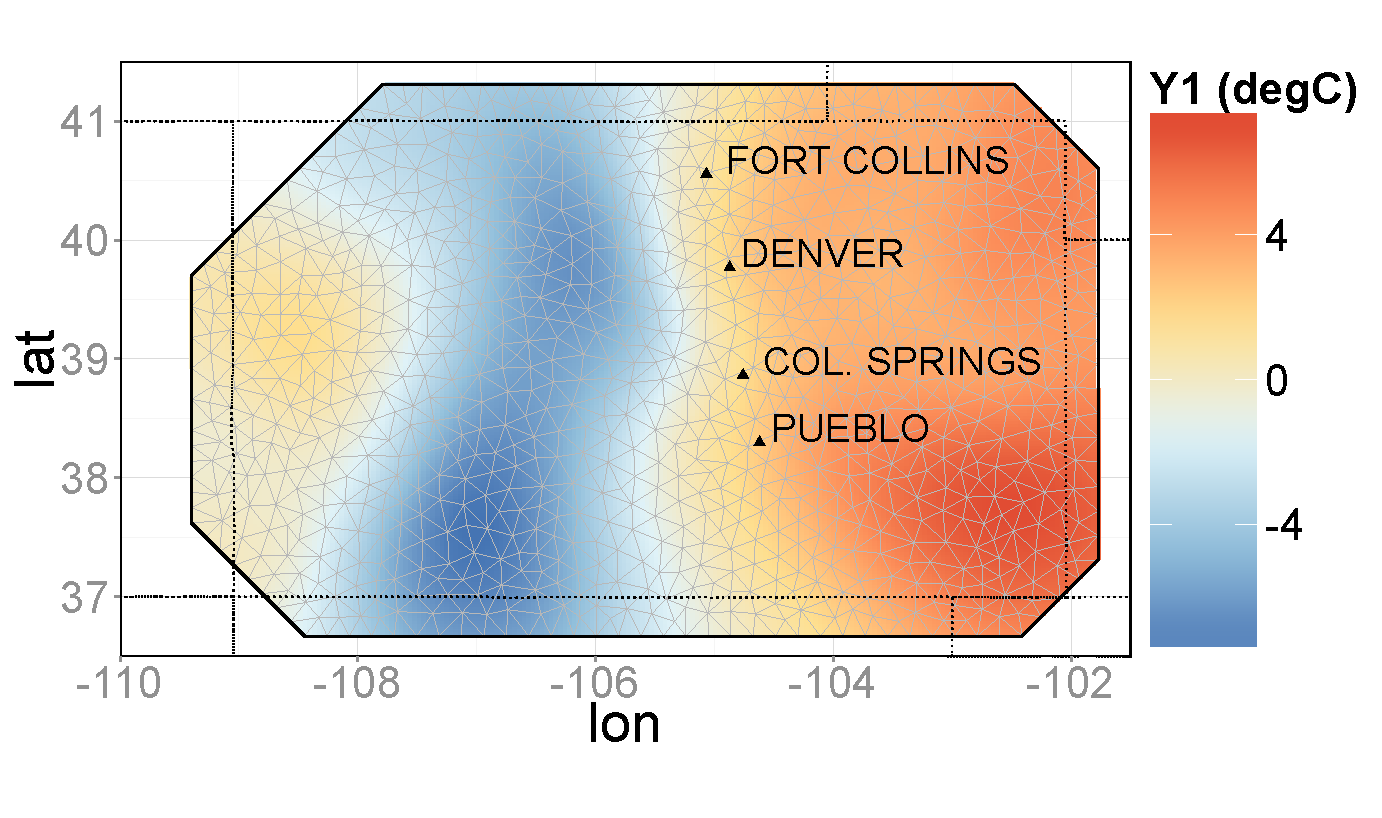
\includegraphics[width=3in]{Fig3a1.png}
\caption{Interpolated map in degrees Celsius (degC) of $\E(\Yvec_1 \mid  \Zvec_1,\Zvec_2)$.}
\end{figure}
\end{frame}

\begin{frame}
\frametitle{Median fields}
\begin{figure}
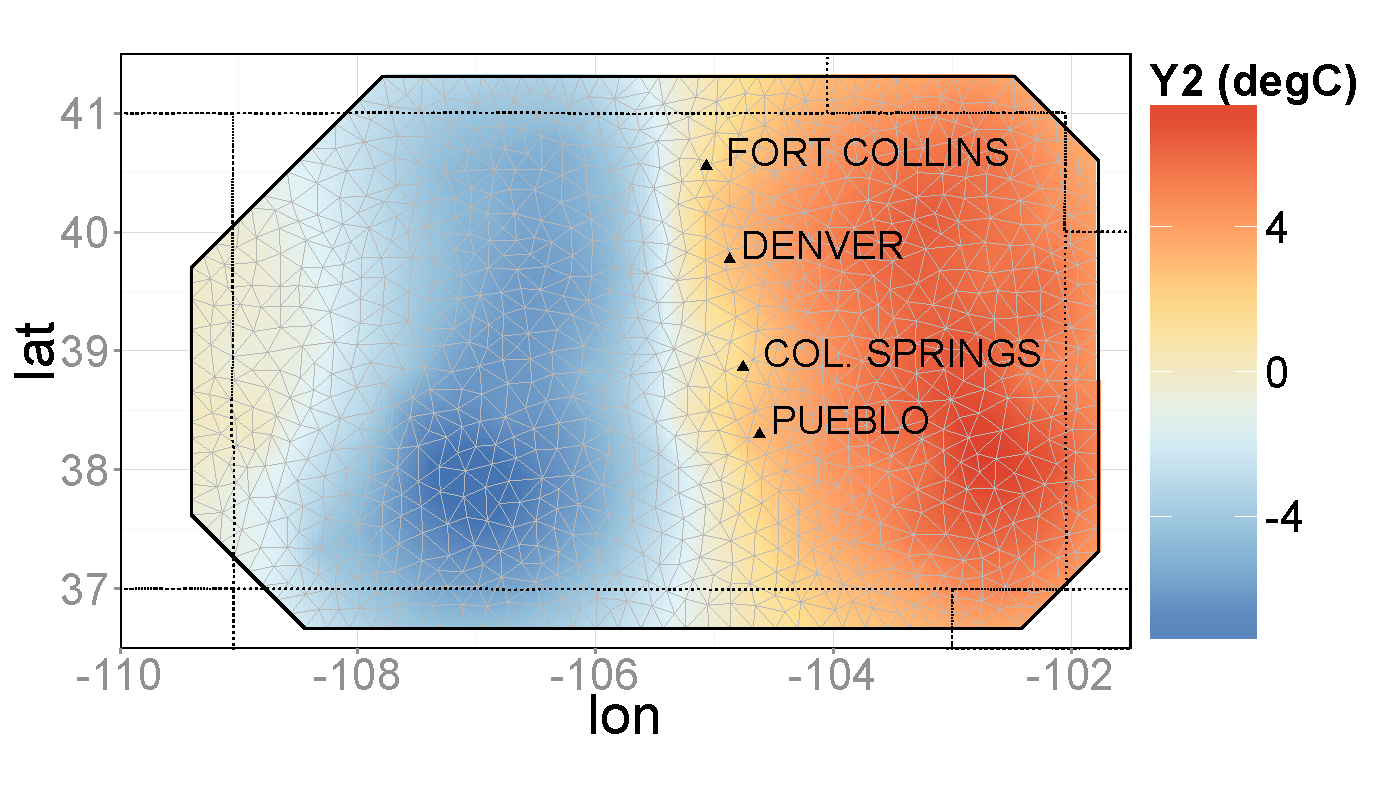
\includegraphics[width=3in]{Fig3a2.png}
\caption{Interpolated map in degrees Celsius (degC) of $\E(\Yvec_2 \mid  \Zvec_1,\Zvec_2)$.}
\end{figure}
\end{frame}


\begin{frame}
\frametitle{Interaction function}


\vspace{-0.1in}
\begin{figure}
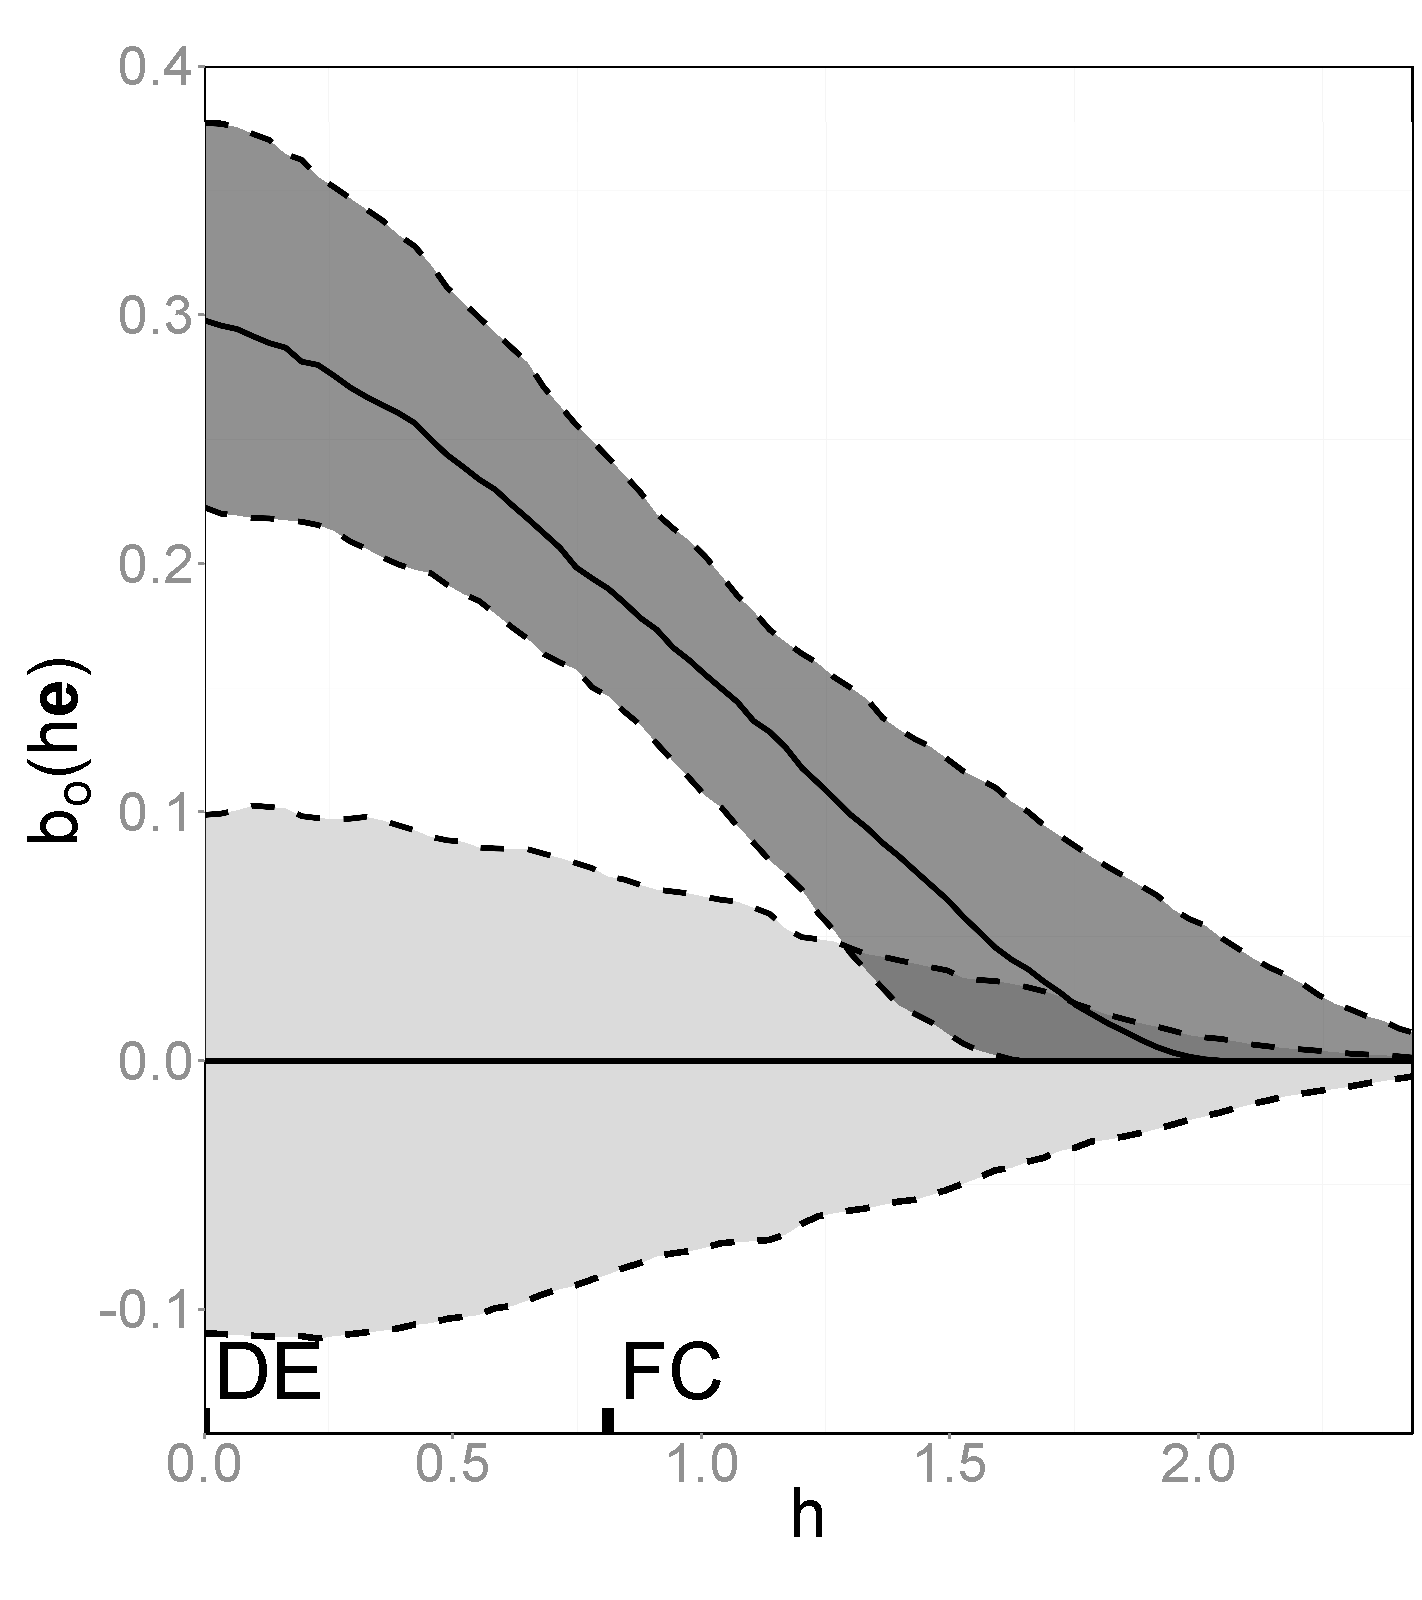
\includegraphics[width=2in]{Fig3b.png}
\caption{\small Prior (light grey) and posterior (dark grey) median (solid line) and inter-quartile ranges (enclosed by dashed lines) of the interaction function $b_o(\cdot)$ of Model 3, along a unit vector $\mathbf{e}$ originating at Denver (DE) in the direction of Fort Collins (FC)} 
\end{figure}

\end{frame}

\normalsize

% ###################

\section{Atmospheric trace-gas inversion in the UK and Ireland}


\begin{frame}
\sectionpage
\end{frame}

\begin{frame}
\frametitle{Atmospheric trace-gas inversion}

\begin{itemize}
\item $Y_1(\svec)$ is methane emissions per unit area -- this is approximately temporally invariant. \vfill
\item $Y_{2,t}(\svec)$ is methane mole fraction and is spatio-temporally varying. \vfill
%\item Only the mole fractions are observed. \vfill
\item {\bf Aim:} Infer the (spatial) emissions from observation of (spatio-temporal) mole fraction.\vfill
%\item Interaction function (SRR) $b_t(\svec,\uvec)$ is the influence of the emissions on the methane, affected by weather, pressure systems etc.\vfill
%\item Methane is a greenhouse gas which absorbs 100x more heat than CO$_2$. 
\end{itemize}
\end{frame}

\begin{frame}
\frametitle{The interaction function}

\begin{itemize}
\item The interaction function is obtained from a Lagrangian particle dispersion simulator (Met Office's NAME).
\end{itemize}

\begin{center}
\begin{figure}
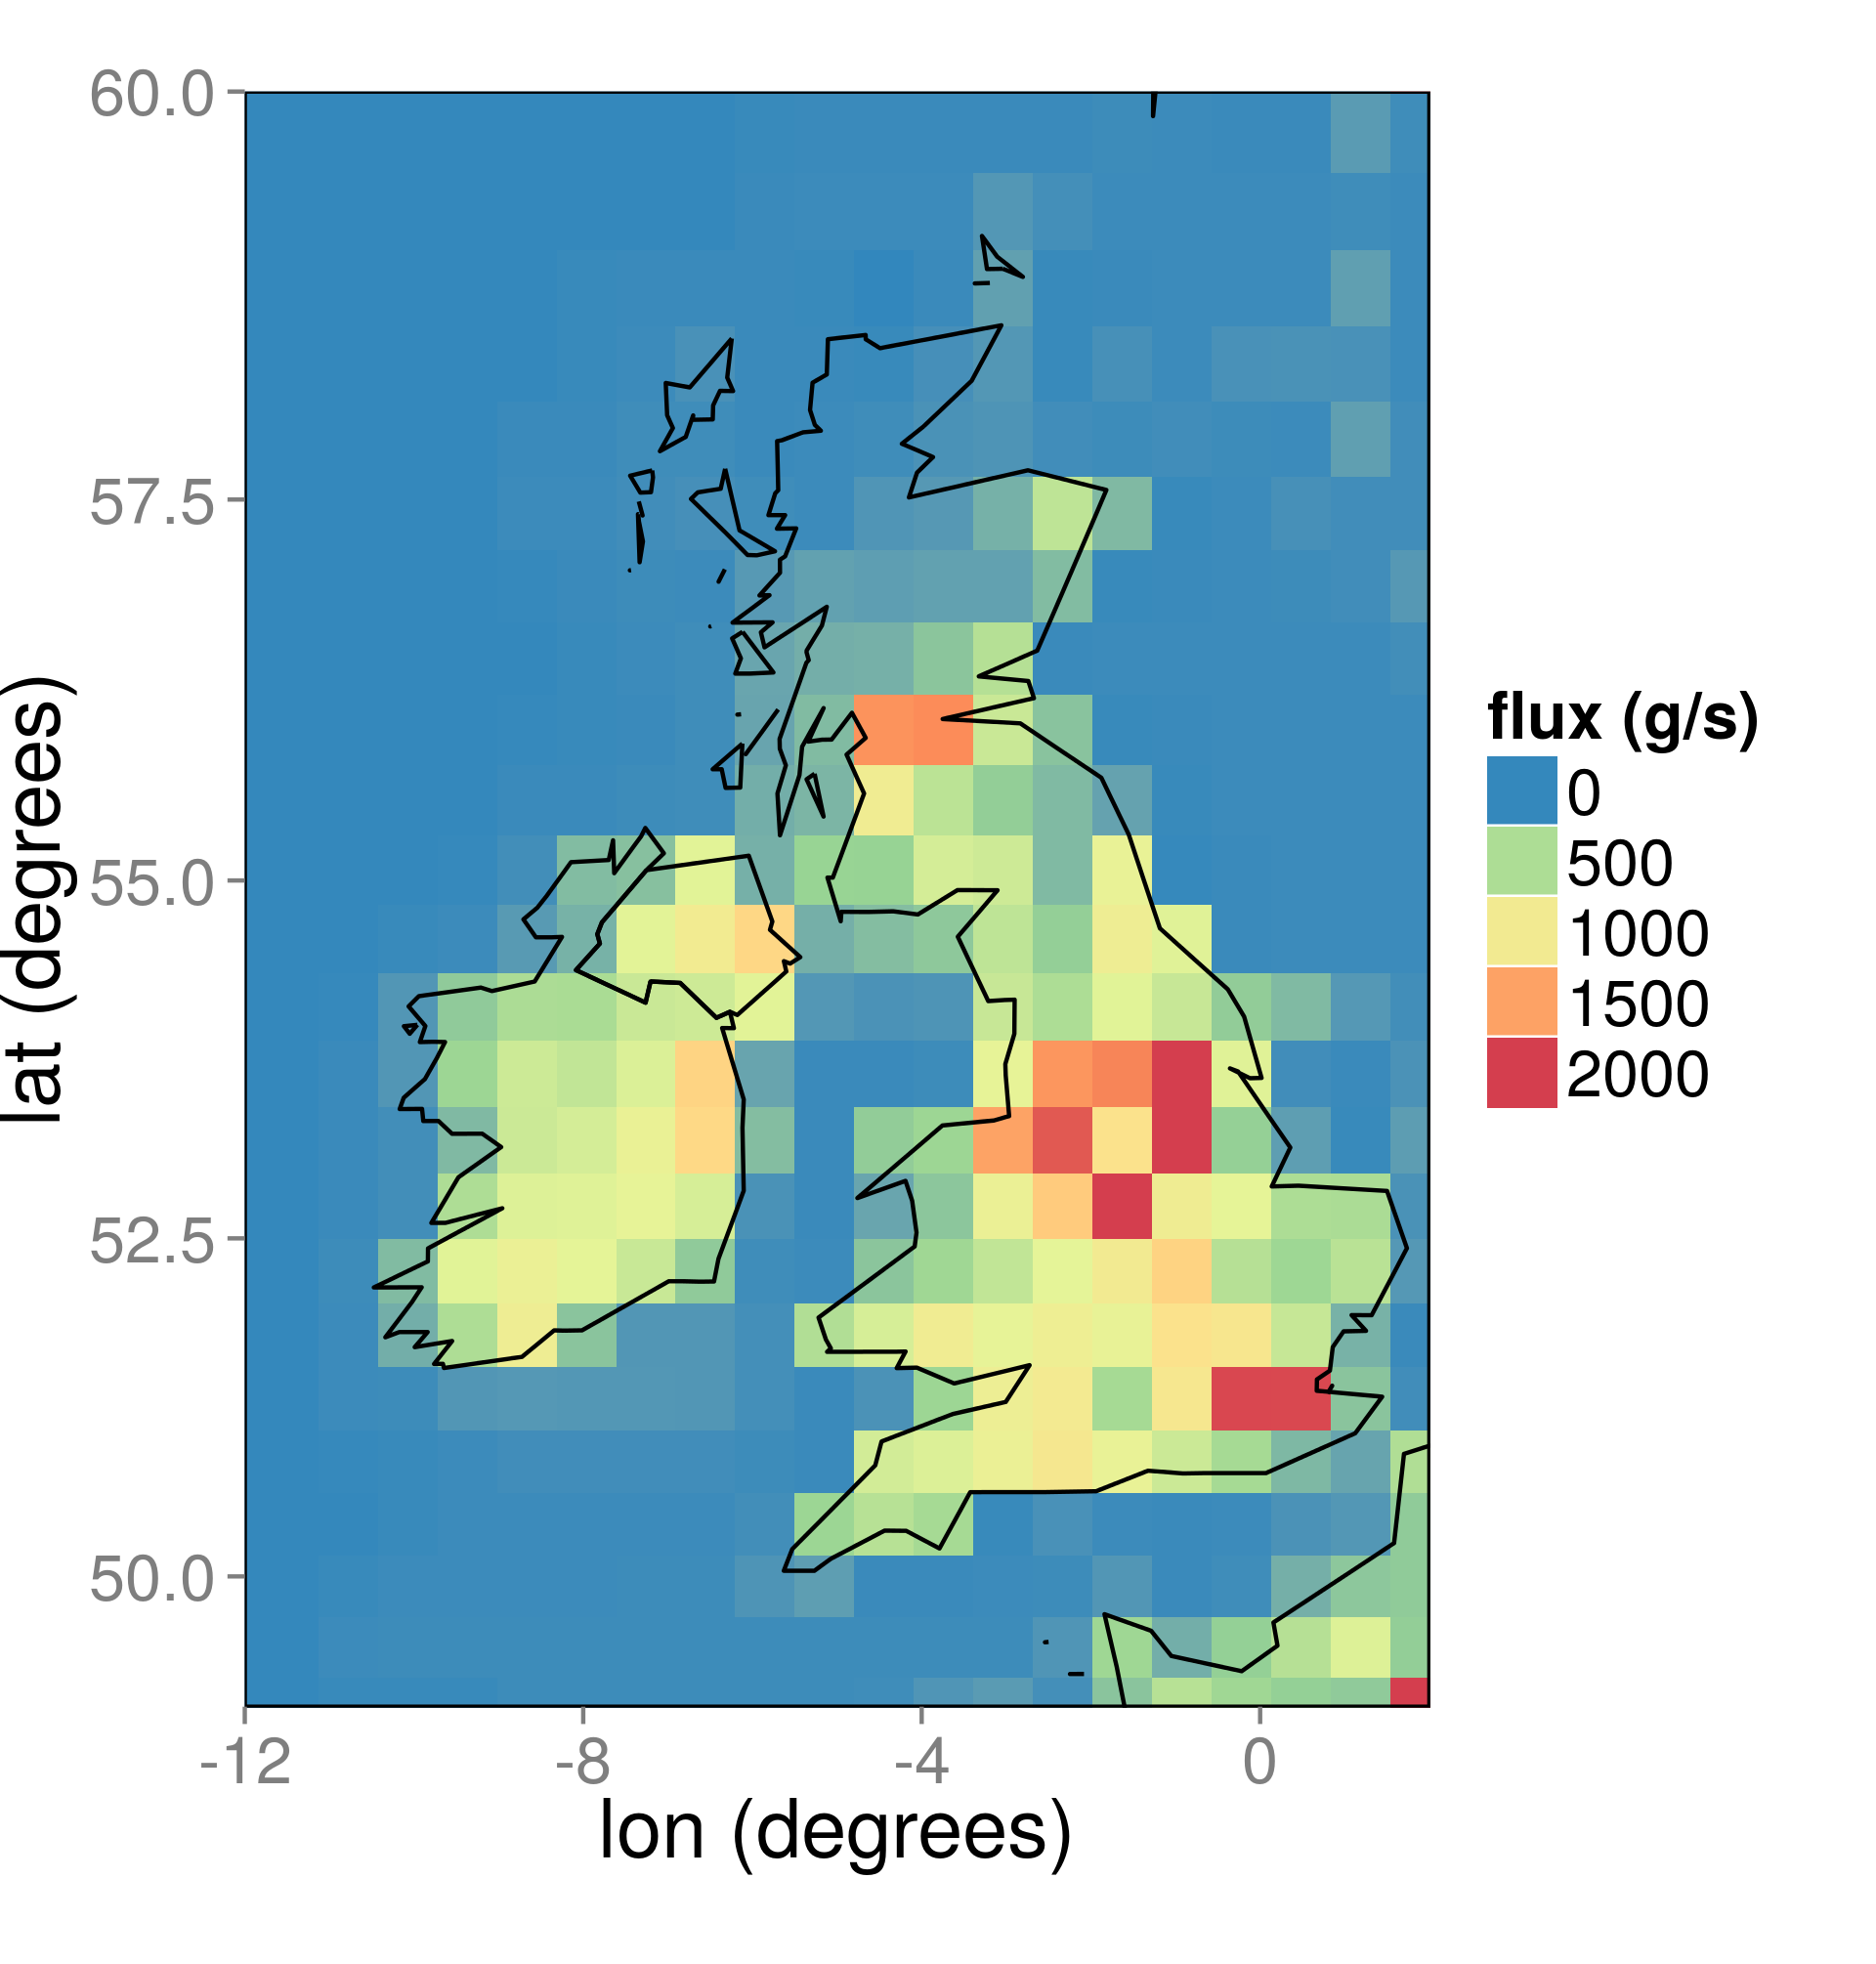
\includegraphics[width=1.5in]{NAEI.png}  
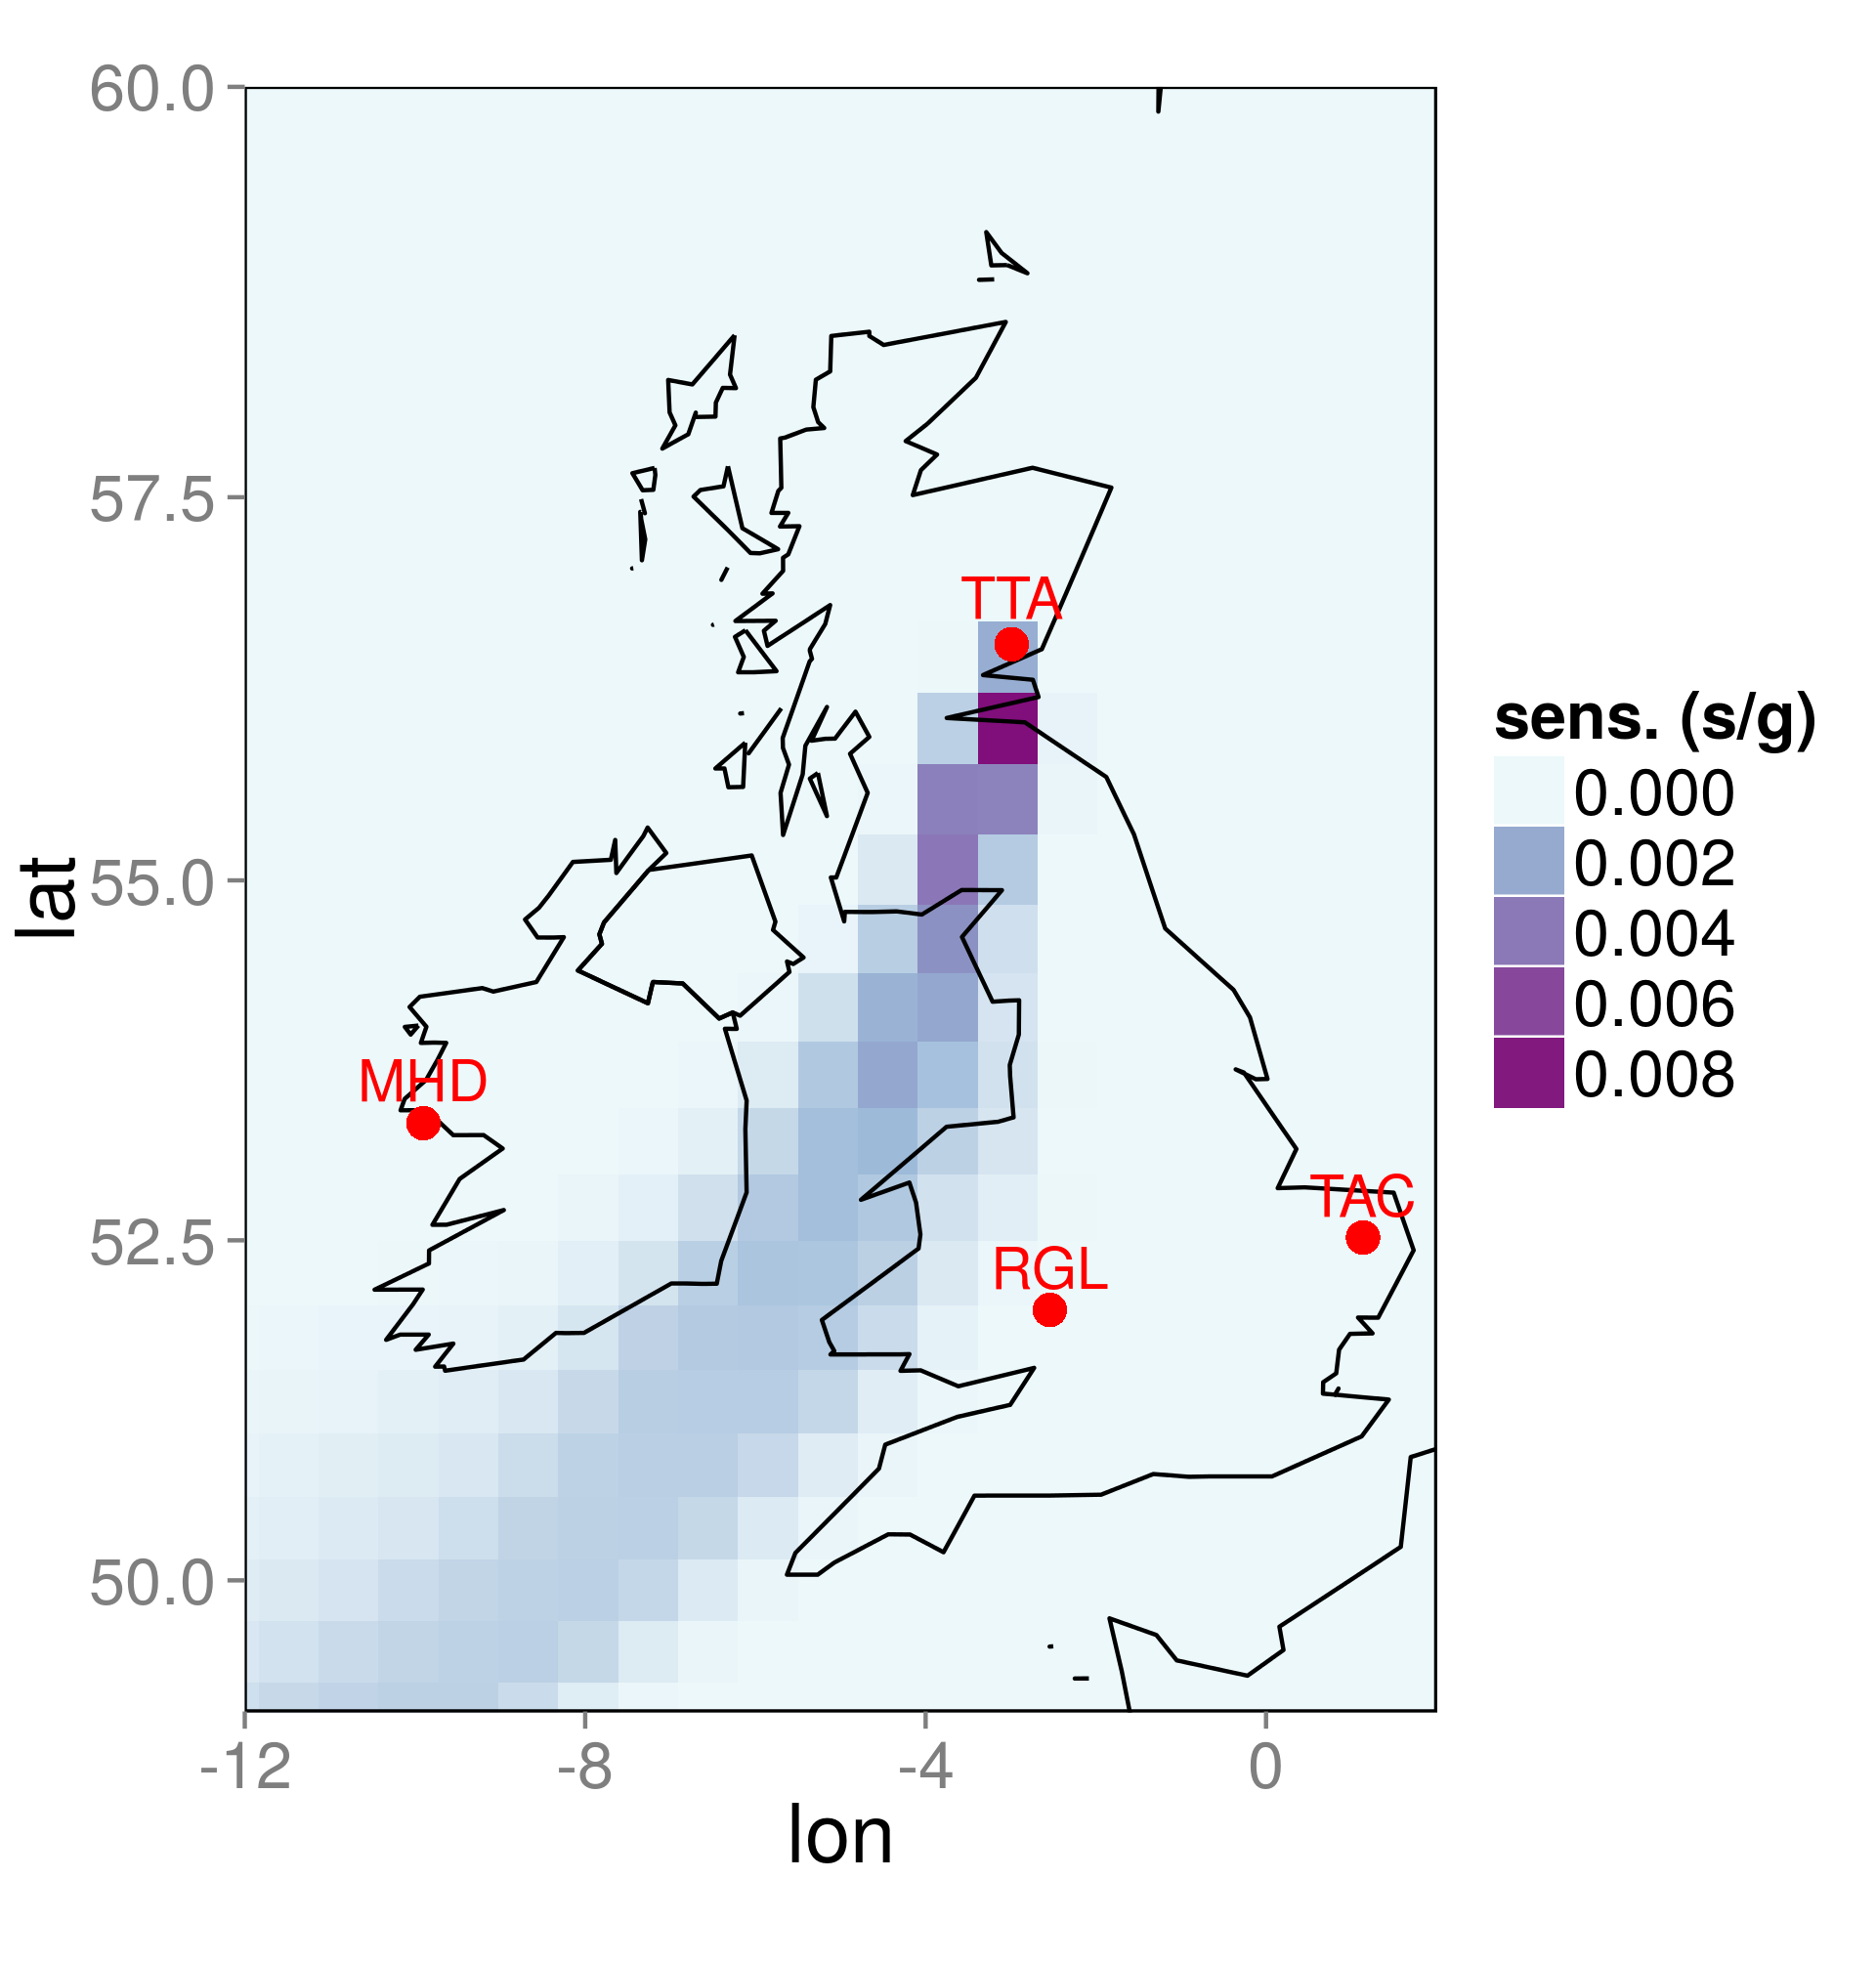
\includegraphics[width=1.5in]{TAC_01_01.png}
\caption{Emissions map obtained from the NAEI for January 2014 (left panel) and the interaction function $b_t(\s,\cdot)$ obtained from the Met Office's NAME  with $\s$ set to the coordinates of the Angus measurement station (\textsc{TTA}), Scotland (right panel).}
\end{figure}
\end{center}
\end{frame}


% #####################

\begin{frame}
\frametitle{Isolated measurements}

\begin{center}
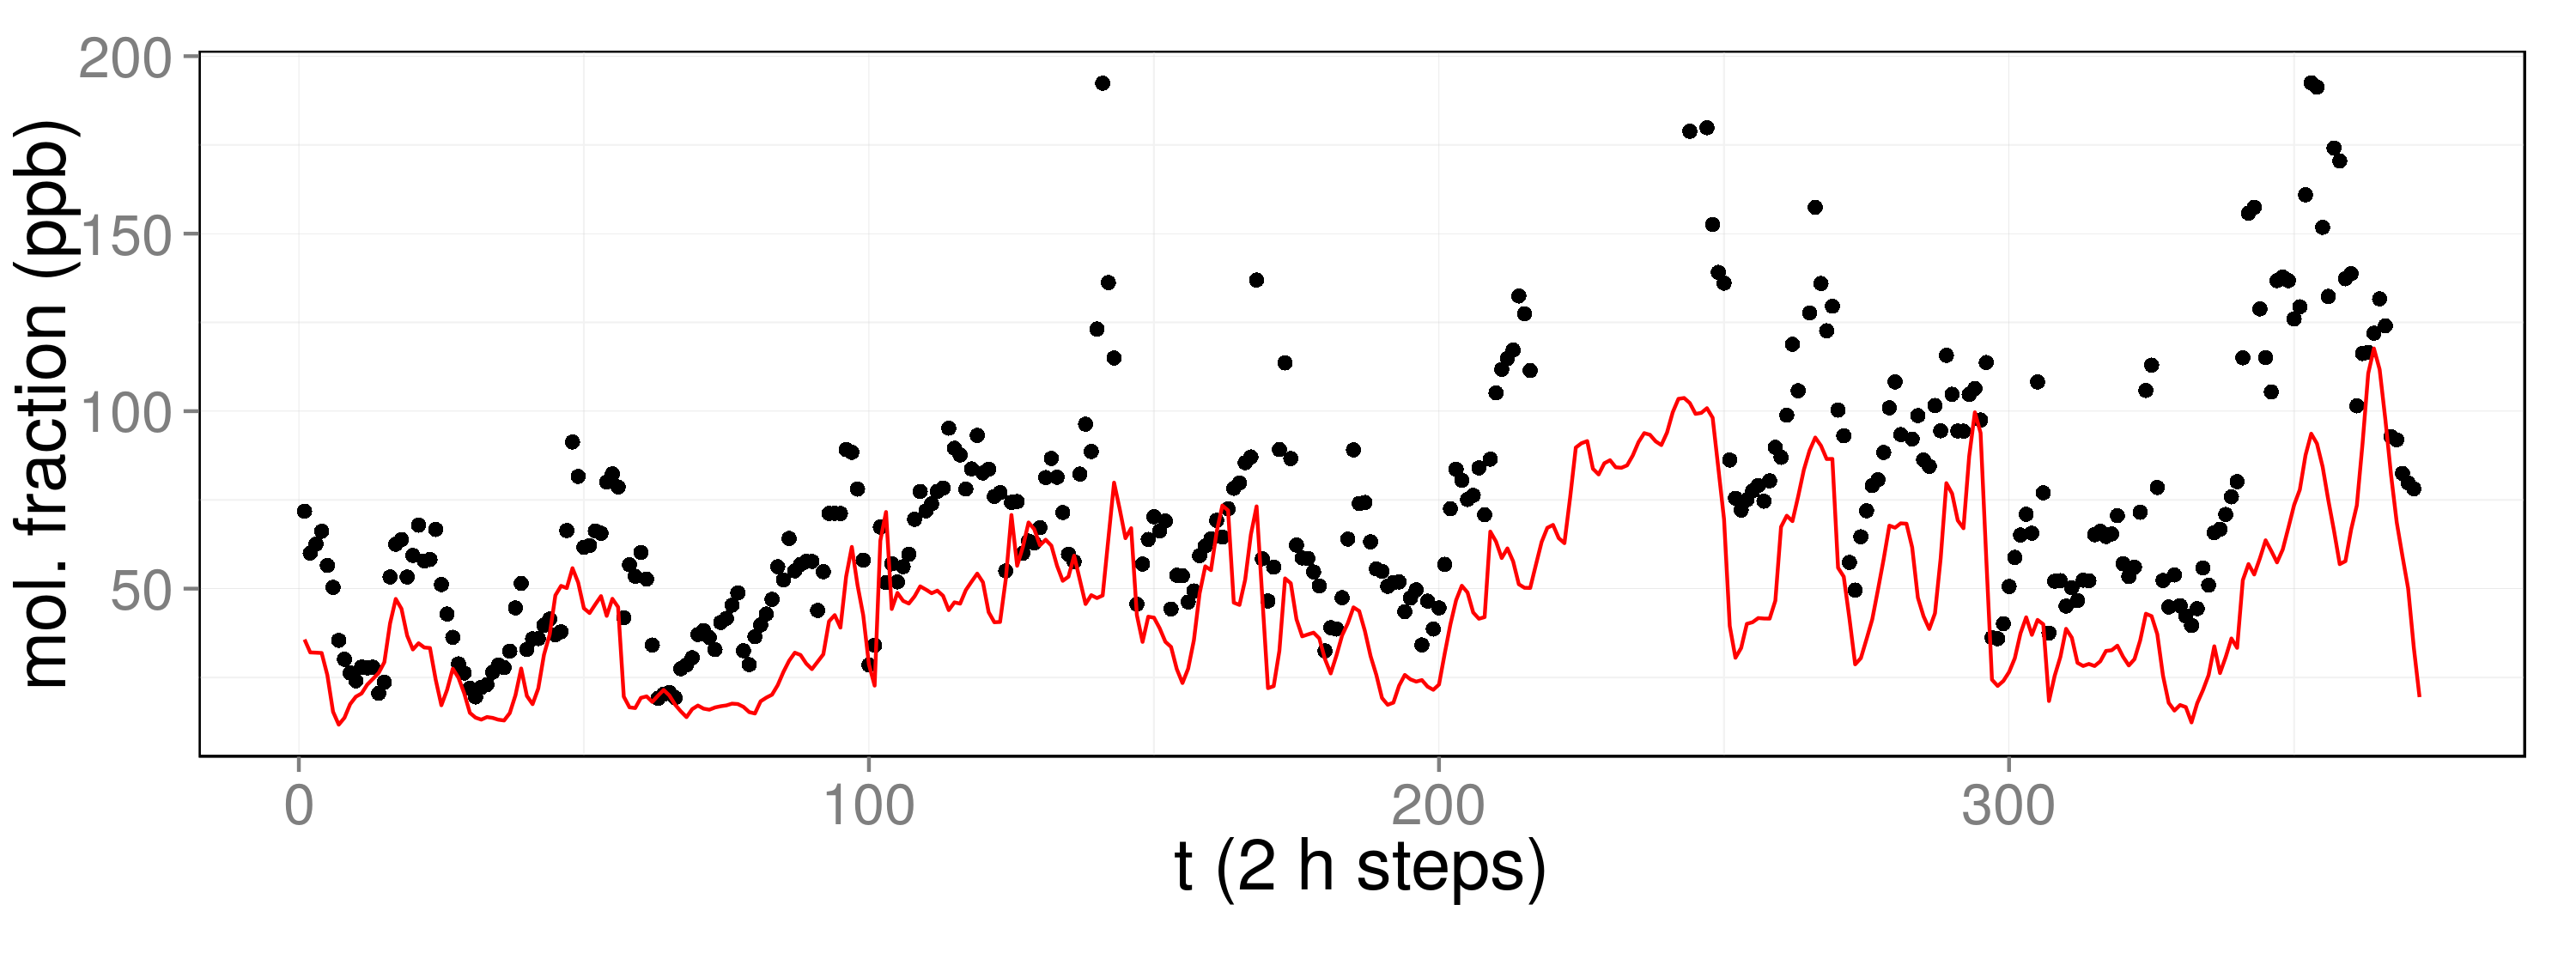
\includegraphics[width=4in]{TAC_01.png}  
\end{center}

\vspace{-1cm}

\begin{itemize}
\small
\item The inversion is an ill-posed problem: We need to estimate a (spatial) emissions field from measurements that aggregate spatio-temporally.
%\item Current methods use data assimilation methods with prior expectations set to what is reported in the inventories.
%\item Inversions are sometimes orders of magnitude off.
\end{itemize}

\normalsize

\end{frame}

\begin{frame}
\frametitle{Emissions are positive}

\begin{itemize}

\item Let $Y_1(\svec)$ be a lognormal spatial process, that is, $\widetilde{Y}_1(\cdot) \equiv \log Y_1(\cdot)$ is a Gaussian process.
\item Let $\E(\widetilde{Y}_1(\s)) \equiv \widetilde\mu_1(\s;\varthetab)$ and $\cov(\widetilde{Y}_1(\s),\widetilde{Y}_1(\u)) \equiv \widetilde{C}_{11}(\s,\u; \varthetab)$.
\begin{align*}
\mu_1(\s;\varthetab) &\equiv \E(Y_1(\s)) \\ &\equiv  \exp(\widetilde{\mu}_1(\svec;\varthetab) + (1/2)\widetilde{C}_{11}(\s,\s;\varthetab)); \quad \svec \in D,\\
&\\
 C_{11}(\s,\u;\varthetab) &\equiv \cov(Y_1(\s),Y_1(\u)) 
\\&\equiv \mu_1(\s;\varthetab)\mu_1(\u;\varthetab)[\exp(\widetilde{C}_{11}(\s,\u;\varthetab)) - 1] ; \quad \svec,\uvec \in D.
\end{align*}
\end{itemize}

\end{frame}

\subsection{Lognormal causal spatio-temporal model}

\begin{frame}
\frametitle{Lognormal bivariate model}

\begin{itemize}

\item We have a causal {\bf spatio-temporal} bivariate model:

\begin{align*}
\E\left(Y_{2,t}(\s)\mid Y_1(\cdot)\right)&\,=\int_D{b_t(\s,\v)Y_1(\v)\,\d \v};\quad \s\in D,\\
\cov\left(Y_{2,t}(\s),Y_{2,t'}(\u)\mid Y_1(\cdot)\right)&\,=C_{2\mid 1,t,t'}(\s,\u);\quad \s,\u\in \mathbb{R}^d,
\end{align*}
with the mole-fraction covariance:

\begin{equation*}
C_{22,t,t'}(\s,\u) = C_{2\mid 1,t,t'}(\s,\u)+\int_D\int_D {b_t(\s,\v)} {C_{11}(\v,\w)} {b_{t'}(\w,\u)}\d\v\d\w.
\end{equation*}

\item The conditional covariance $C_{2\mid 1,t,t'}$ is used to account for simulator discrepancy (boundary conditions, model discretisation, linearisation, etc.).

\end{itemize}

\end{frame}


\begin{frame}
\frametitle{Expectations and covariances}

\begin{align*}
\Yvec_t(\cdot) \sim \Dist\begin{pmatrix} \begin{pmatrix} \mu_1(\cdot) \\ \mu_{2,t}(\cdot) \end{pmatrix},\begin{pmatrix}  C_{11}(\cdot,\cdot) &  C_{12,t'}(\cdot,\cdot) \\  C_{21,t}(\cdot,\cdot) &  C_{22,t,t'}(\cdot,\cdot) \end{pmatrix} \end{pmatrix},\quad t,t' \in \mathbb{R}^+.
\end{align*}

\begin{itemize}
%\item Our problem is the size of $\bSigma$, which can become very large.
\item What to choose for $C_{2|1,t,t'}(\svec,\uvec)$? \vfill
\item \emph{Strategy 1}: If dim$(\Zvec_{2,t}) < 10$, say, then use standard spatio-temporal covariance functions, which yield (dense) covariance matrices, and evaluate $Y_{2,t}(\cdot)$ only where we take observations. \vfill
\item \emph{Strategy 2}: If dim$(\Zvec_{2,t}) \gg 10$, then we need to use sequential estimation methods,  dimensionality reduction and/or {\bf matrix sparsity}. \vfill
\end{itemize}
\end{frame}

\begin{frame}
\frametitle{Model 1}

\begin{itemize}

\item The discrepancy is a separable spatio-temporal Gaussian process with
\begin{align*}
C_{2|1,t,t'}(\svec,\uvec) &= \sigma^2_{2|1}\rho_s(\svec,\uvec; d)\rho_t(t,t'; a),\\
\rho_s(\svec,\uvec; d) &\equiv \exp(\| \svec - \uvec \| / d);\quad d>0, \\
\rho_t(t,t'; a) &\equiv a^{|t - t'|}; \quad |a| < 1,
\end{align*}

\item Then $\bSigma_{2|1} = \sigma^2_{2|1} \widetilde\bSigma_{2|1,t} \otimes \widetilde\bSigma_{2|1,s}$.
\item $\Bmat$ is obtained by concatenating $\{\Bmat_t: t = 1,2,\dots\}$
\begin{equation*}
\bSigma = 
\begin{pmatrix}
\bSigma_{11} & \bSigma_{11}\Bmat' \\
\Bmat \bSigma_{11} & \Bmat \bSigma_{11}\Bmat' + \bSigma_{2|1}
\end{pmatrix}.
\end{equation*}.

\item $\Bmat$ is dense: Sparse covariance matrices are not of any use.

\end{itemize}

\end{frame}


\begin{frame}
\frametitle{Model 2}

\begin{equation*}
\bSigma^{-1} = \begin{pmatrix} 
\Bmat'\Qmat_{2|1}\Bmat + \Qmat_{11} & -\Bmat'\Qmat_{2|1} \\
-\Qmat_{2|1}\Bmat & \Qmat_{2|1}
\end{pmatrix}.
\end{equation*}

\begin{itemize}
\item Large benefit by making sure the (very large) matrix $\Qmat_{2|1}$ is sparse.
\pause \item We define
\begin{equation*}
\Qmat_{2|1} \equiv \sigma_{2|1}^{-2}\widetilde\Qmat_{2|1,t} \otimes \widetilde\Qmat_{2|1,s}~~,
\end{equation*}
\noindent where
\begin{equation*}
\widetilde\Qmat_{2|1,t} \equiv \begin{pmatrix} 1 & -a &0&&&& 0\\ -a & (1 + a^2) & -a &&&&0  \\ &&&\ddots&&& \\ 0&&&& -a& (1 + a^2) & -a \\ 0&&&&0&-a & 1 \end{pmatrix}.
\end{equation*}
\noindent and we get $\Qmat_{2|1,s}$ from an intrinsic Gaussian Markov random field specification.
\end{itemize}
\end{frame}

\begin{frame}
\frametitle{$\bSigma^{-1}$ is sparse}

\begin{equation*}
\bSigma^{-1} = \begin{pmatrix} 
\Bmat'\Qmat_{2|1}\Bmat + \Qmat_{11} & -\Bmat'\Qmat_{2|1} \\
-\Qmat_{2|1}\Bmat & \Qmat_{2|1}
\end{pmatrix}.
\end{equation*}

\begin{center}
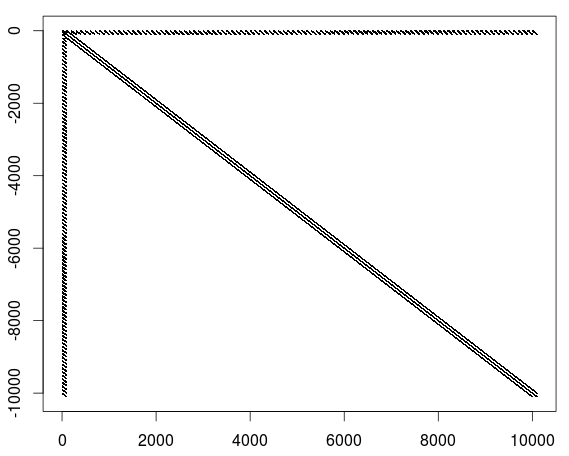
\includegraphics[width=2.5in]{Qsparse.png}
\end{center}
\end{frame}

\subsection{Inference}

\begin{frame}
\frametitle{Inference}

\begin{itemize}
\item $b_t(\svec,\uvec)$ is assumed known from NAME. \vfill
\item We can obtain reasonable estimates of the parameters appearing in $C_{11}(\svec,\uvec)$ from inventories (range, marginal variance, and nugget). \vfill
\item We have no idea what the parameters appearing in $C_{2|1}(\svec,\uvec)$ are. These need to be estimated. \vfill
\end{itemize}
\end{frame}

\begin{frame}
\frametitle{Computational strategy}

\begin{itemize}
\item This is an ill-posed problem: MCMC chains where both the parameters and the fields are unknown will not mix well. \pause \vfill 
\item We know the first two moments -- use a {\bf Laplace-approximated-EM} to estimate the parameters, then fix the parameters and use MCMC for inferring the fields. \vfill \pause
\item This is known as an empirical hierarchical model \citep[EHM;][]{CressieWikle2011}. \vfill \pause
\item We can compute all the (horrible) gradients analytically, use an MCMC method that takes advantage of these. This is known as Hamiltonian Monte Carlo (HMC). \vfill
\end{itemize}
\end{frame}

\begin{frame}
\frametitle{HMC}

\begin{itemize}
\item Use Hamiltonian dynamics to propose the next state in an MCMC chain \citep{Duane_1987}.
\item Need knowledge of gradient to simulate dynamics.
\item Suitable when variables are highly correlated a posteriori (ill-posed problem).
\item Dynamics are simulated using standard methods (Euler or leapfrog method).
\item One-step updates = Langevin method.
\item HMC chains are ergodic and reversible \citep{Neal_2011}.
\end{itemize}
\end{frame}

\begin{frame}
\frametitle{HMC}

\begin{center}
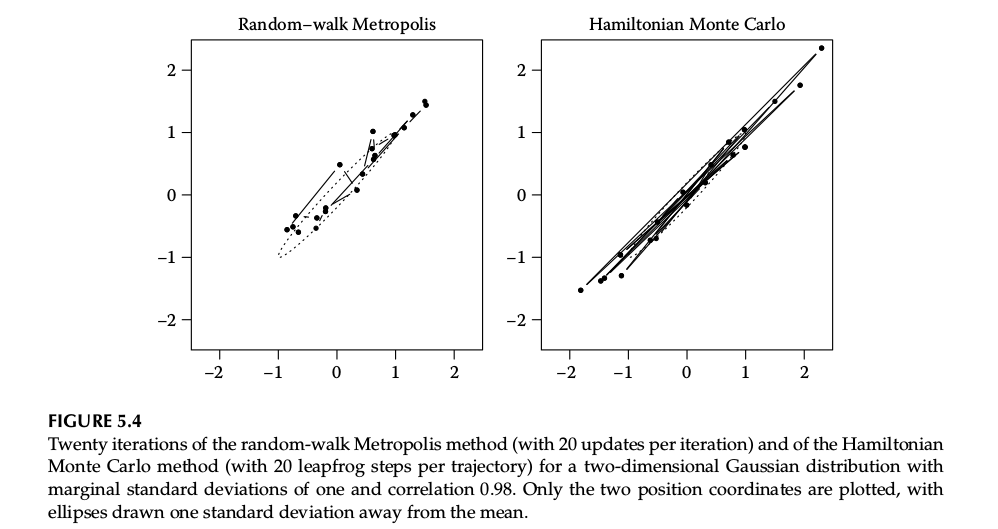
\includegraphics[width=4in]{HMC2.png}
\end{center}
\begin{itemize}
\item Figure taken from \cite{Neal_2011}.
\end{itemize}
\end{frame}


\subsection{Simulation studies}


\begin{frame}
\frametitle{Simulation study}

\begin{enumerate}
\item Assume the properties of the lognormal flux spatial process (i.e., $\widetilde{C}_{11}$ and $\widetilde{\mu}_{1}$ are known), and simulate a realisation. \vfill
\item Simulate a spatio-temporal interaction function (assumed known).\vfill
\item Simulate mole fraction observations at a few locations (Model 1) and at many (1000) locations (Model 2).\vfill
\item Infer the flux $Y_1(\svec)$ from the data in both cases.\vfill
\end{enumerate}
\end{frame}

\begin{frame}
\frametitle{Simulation study}

\begin{itemize}
\item Simulated interaction function.
\end{itemize}

\begin{center}
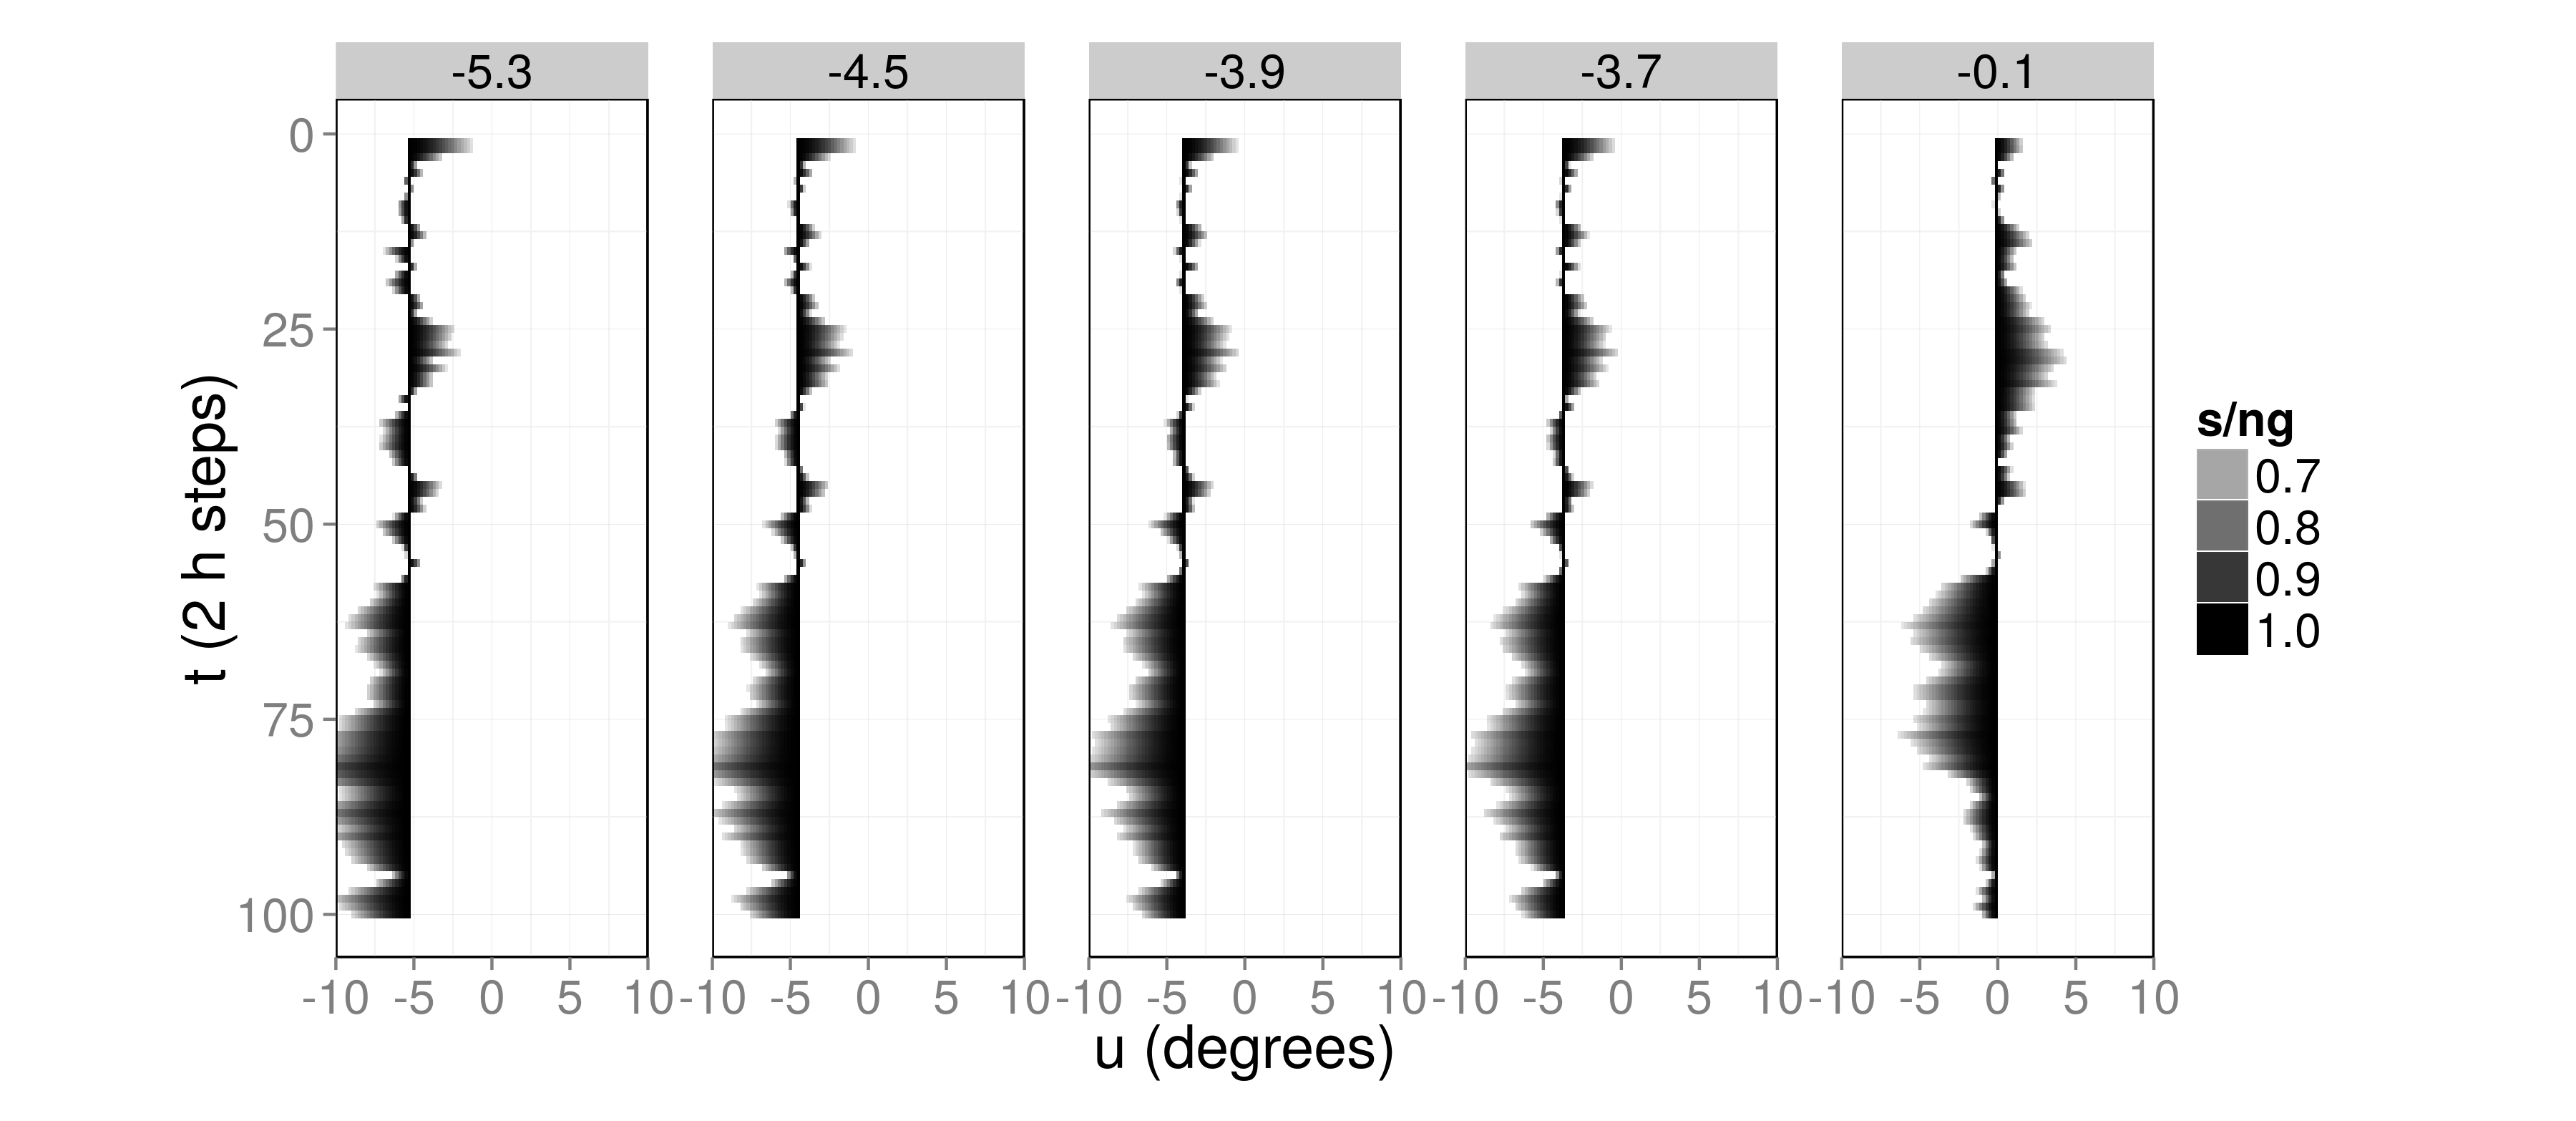
\includegraphics[width=4in]{B_plot.png}
\end{center}
\end{frame}

\begin{frame}
\frametitle{Simulation study}

\begin{itemize}
\item Flux and time-averaged mole-fraction field.
\end{itemize}

\begin{center}
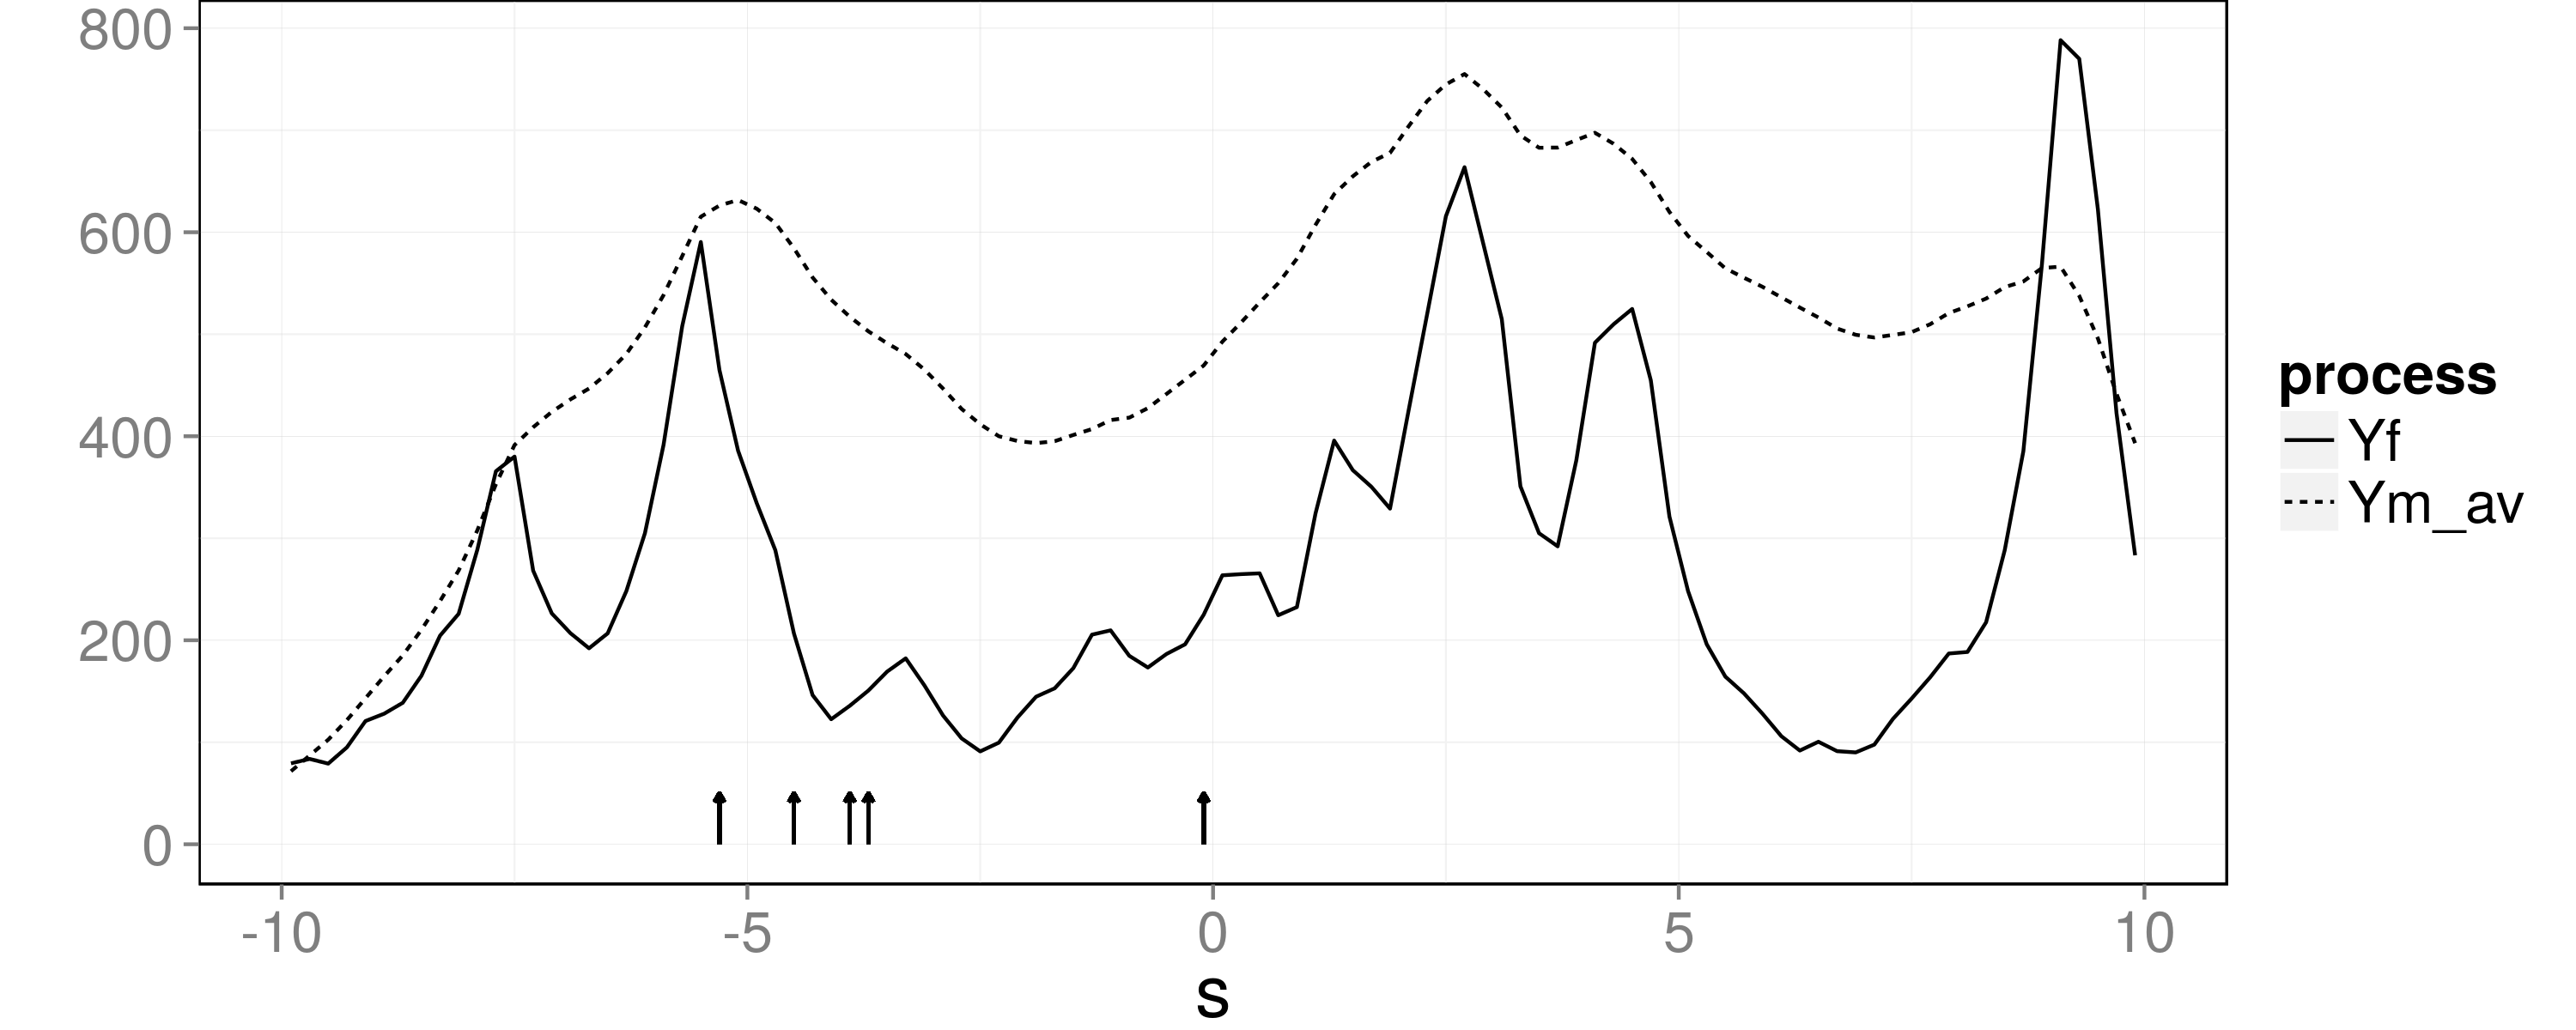
\includegraphics[width=4in]{Sim_plot.png}
\end{center}
\end{frame}

\begin{frame}
\frametitle{Simulation study}

\begin{itemize}
\item Laplace-EM proved relatively straightforward to implement.
\item Convergence with Model 1 $\simeq$ 80 iterations.
\item Convergence with Model 2 $\simeq$ 5 iterations (much more data).
\item Convergence may be hard to achieve when mode is close to zero and tails are heavy (gradient descents with varying tolerance for convergence).
\item ``Bouncing method'' needs to be implemented for the HMC chain to respect positivity constraint \citep{Neal_2011}.
\end{itemize}
\end{frame}


\begin{frame}
\frametitle{Simulation study}

\begin{itemize}
\item Inference on flux field for Model 1 using HMC (10,000 samples).
\end{itemize}

\begin{center}
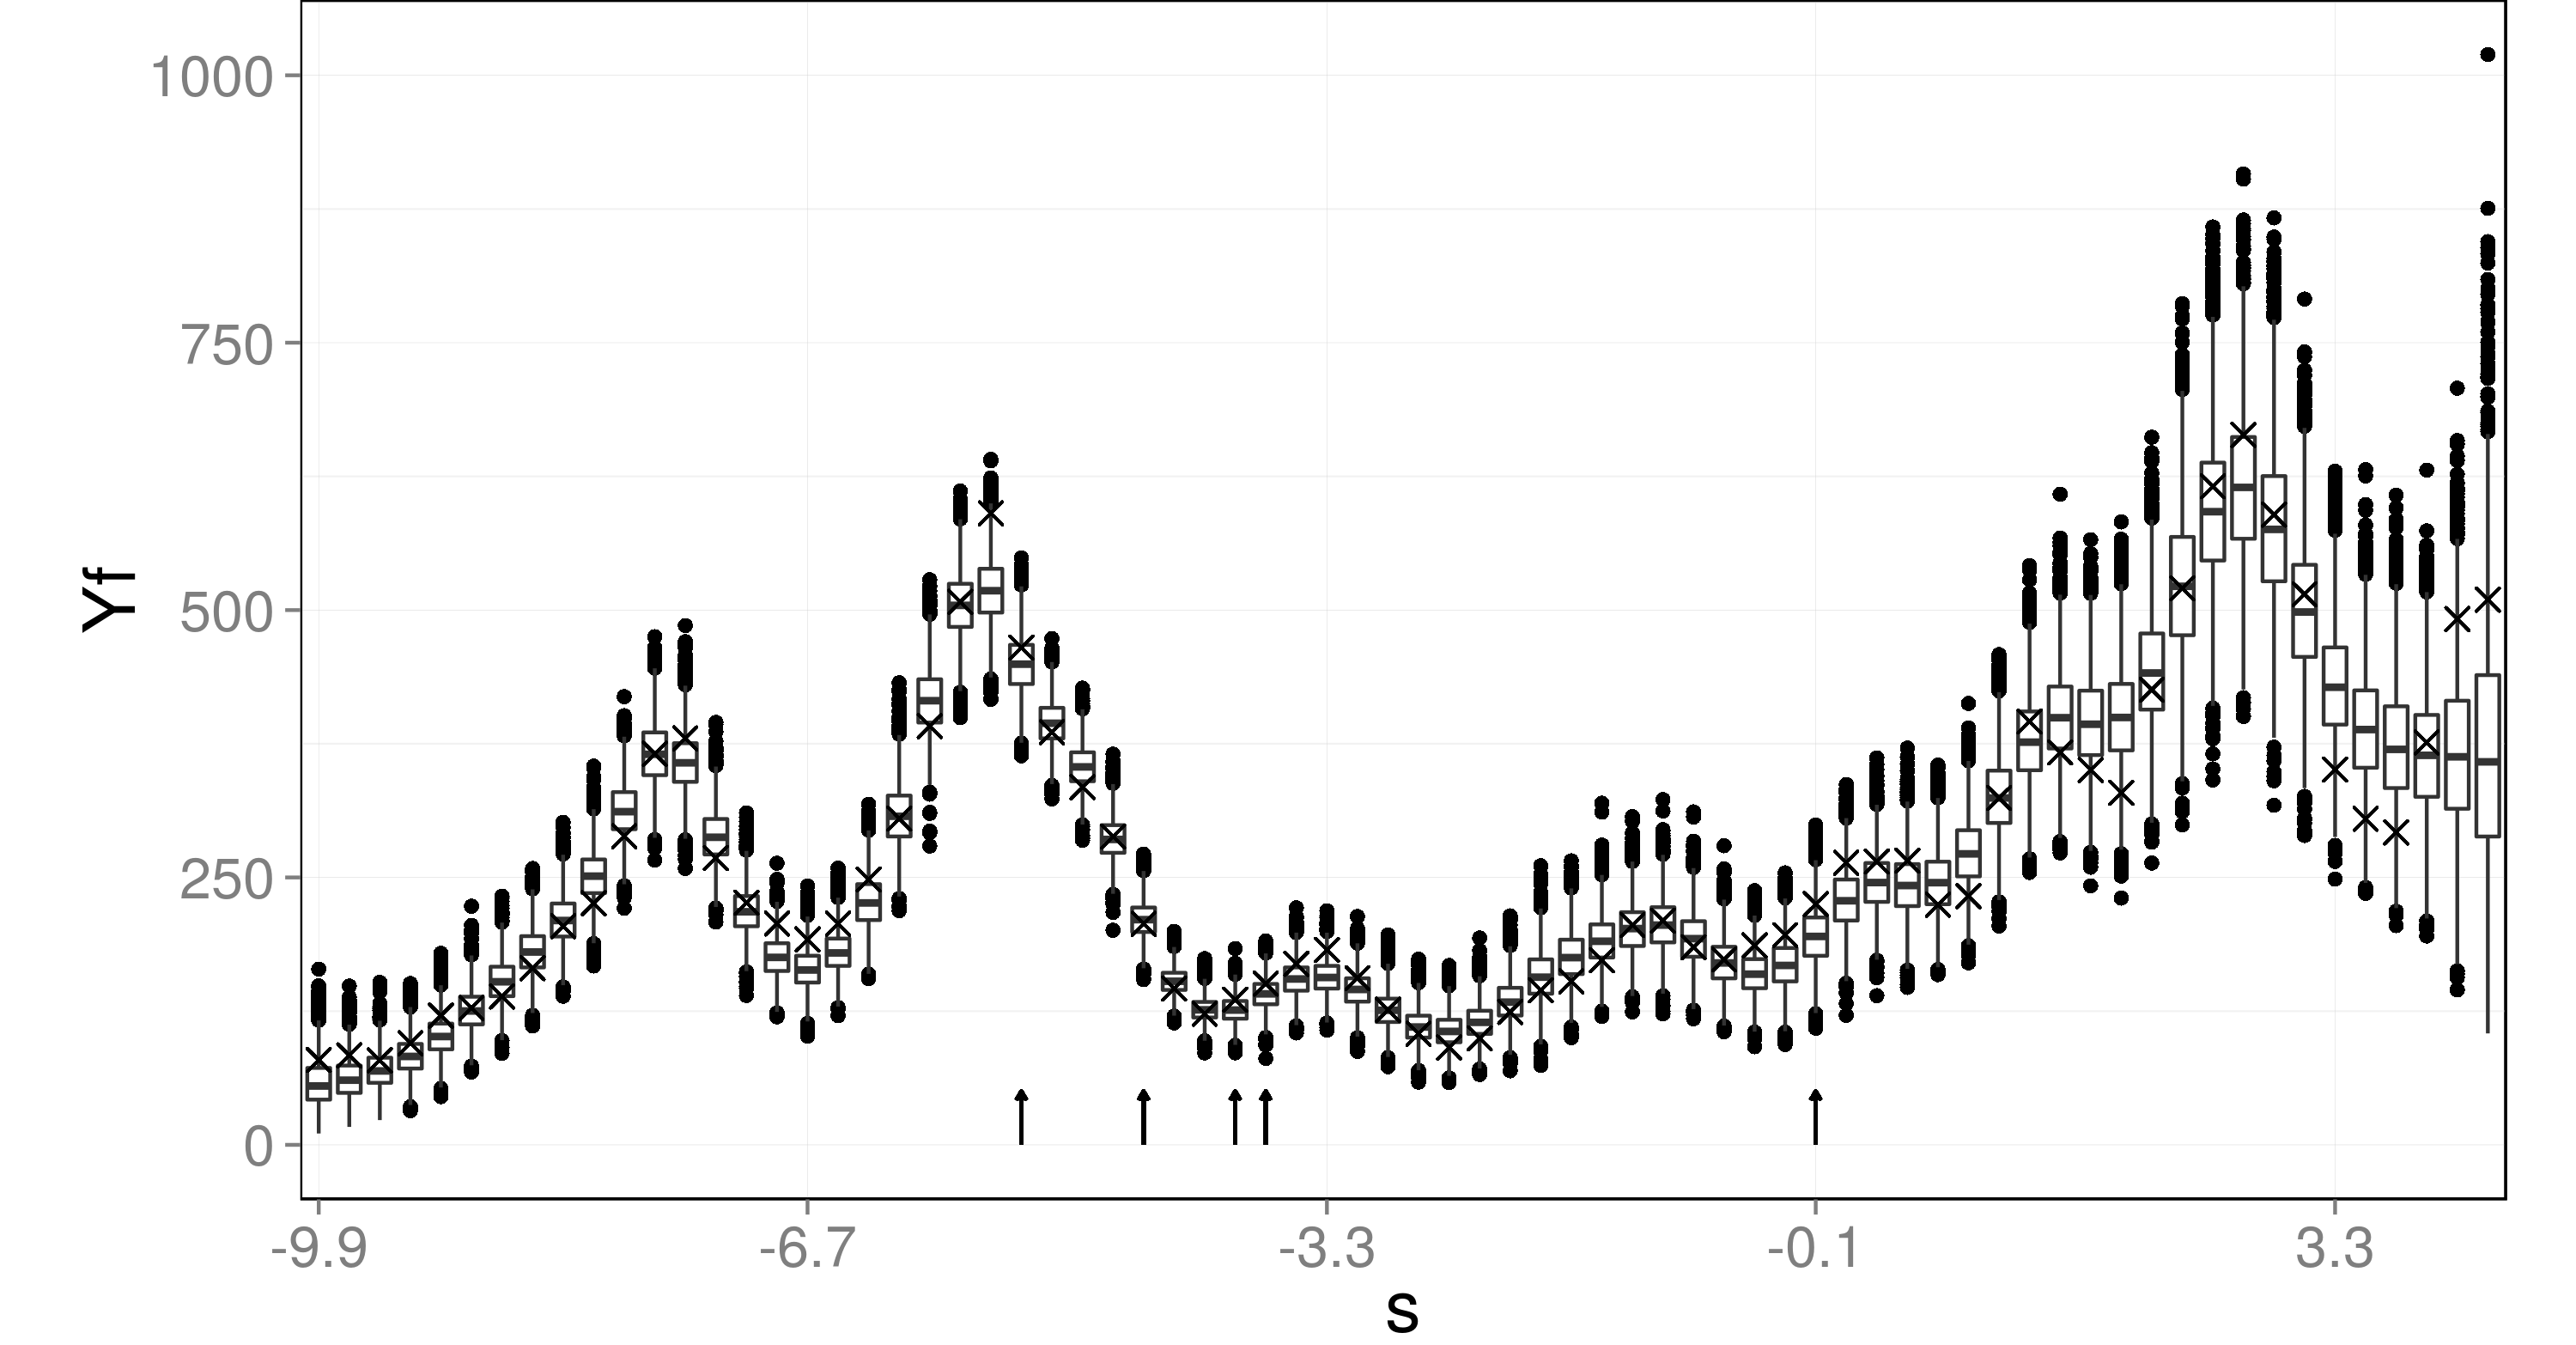
\includegraphics[width=4in]{Sim1_samples.png}
\end{center}
\end{frame}

\begin{frame}
\frametitle{Simulation study}
\begin{itemize}
\item Why include the HMC if we have a Laplace-EM?
\end{itemize}
\begin{center}
\vspace{-0.5cm}
\begin{figure}
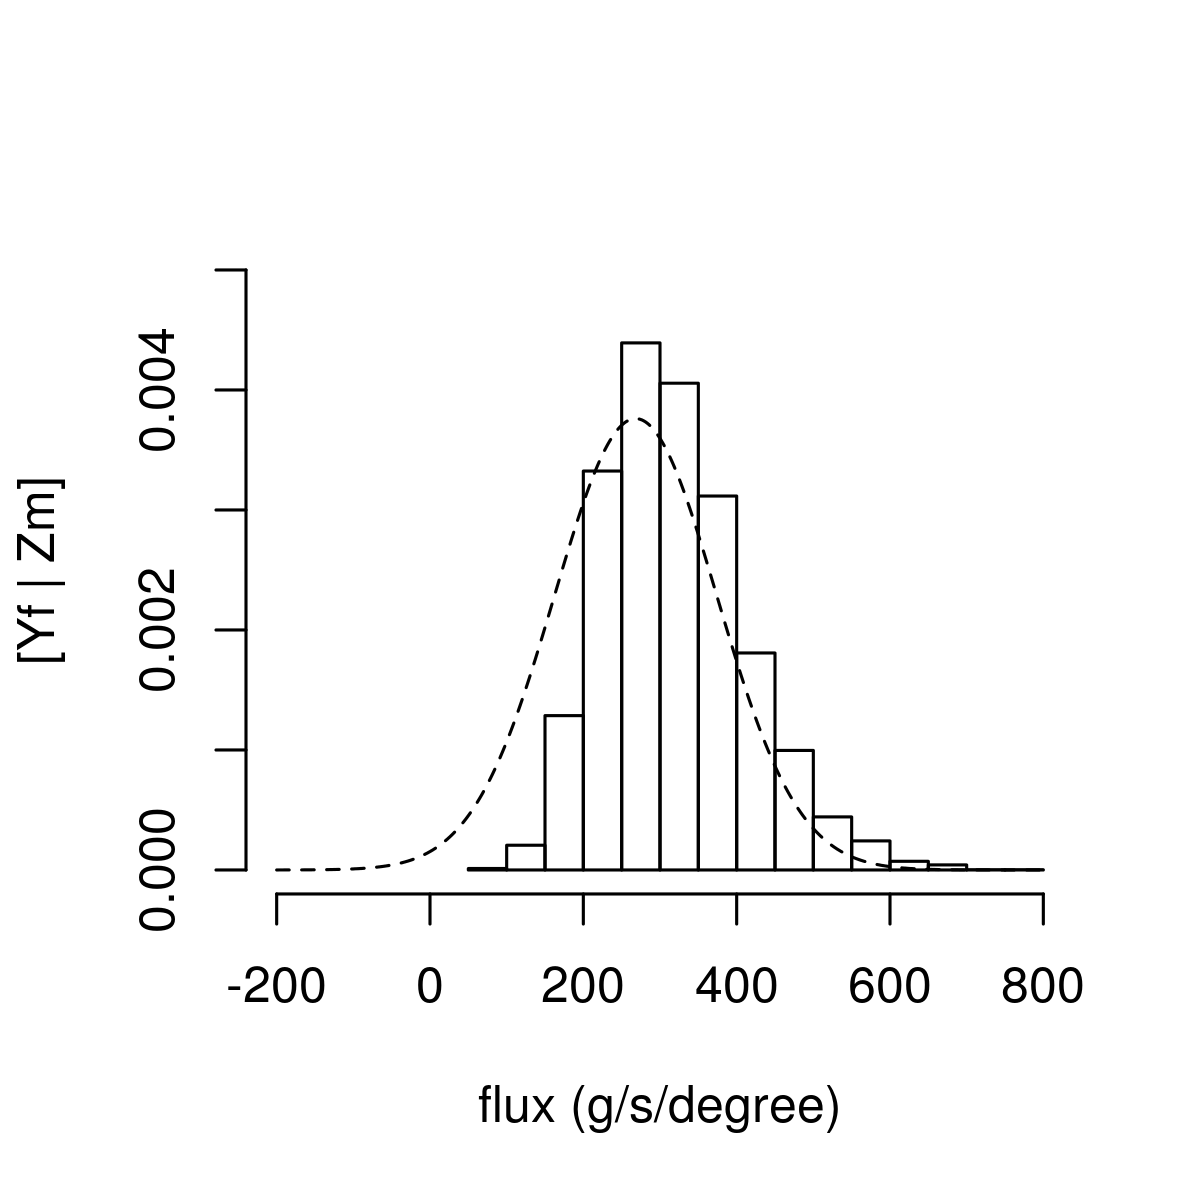
\includegraphics[width=2in]{density_sim1.png}
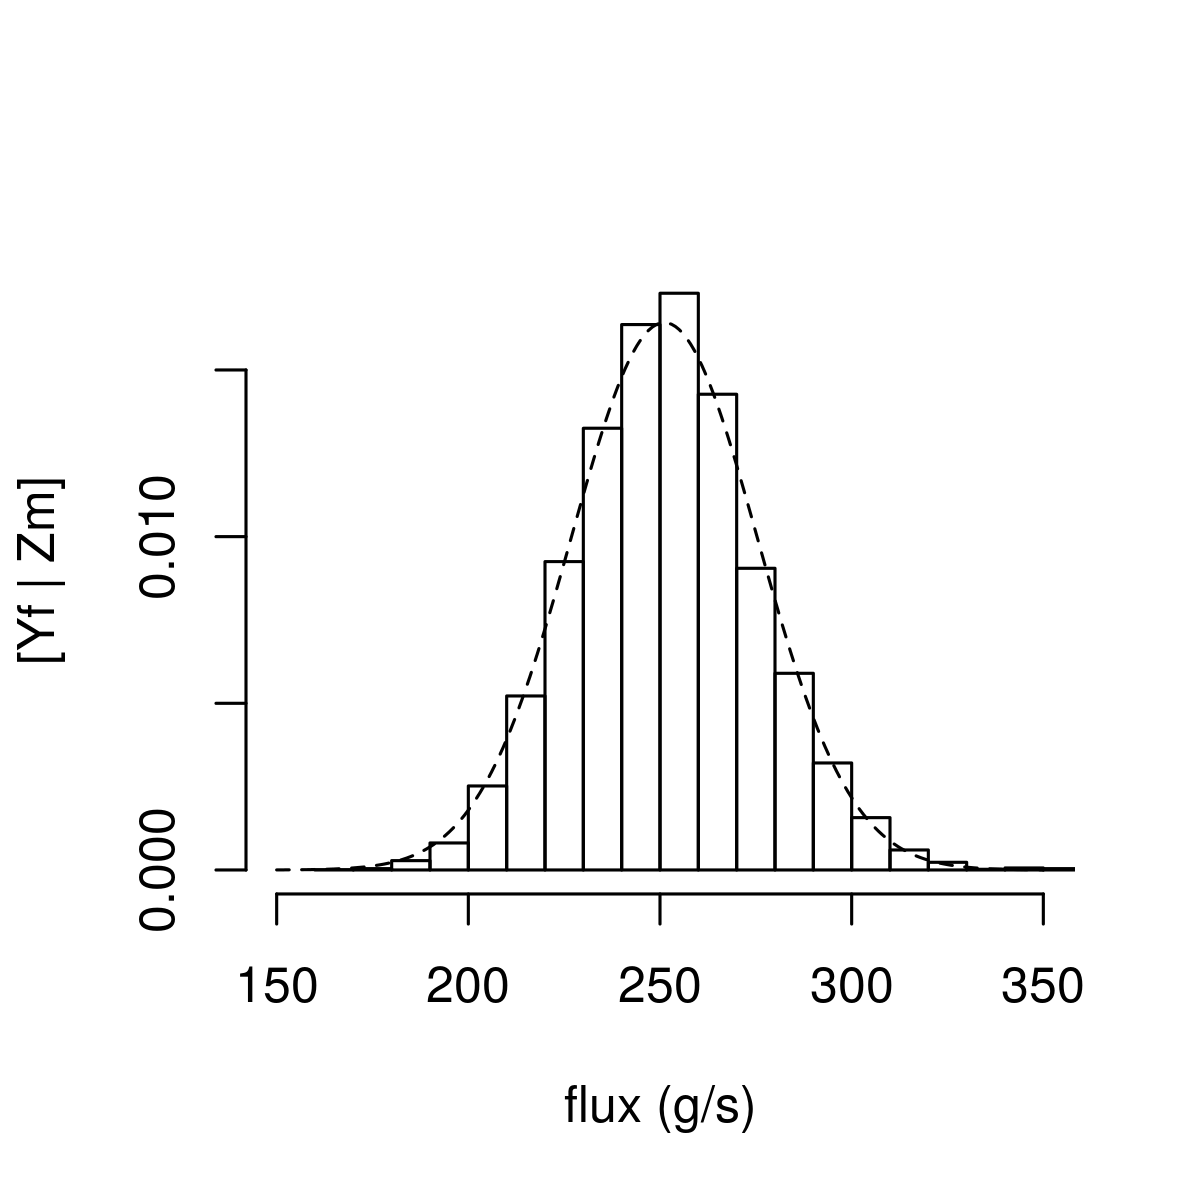
\includegraphics[width=2in]{density_sim10.png}
	\caption{Laplace approximation (dashed line) and a histogram of the empirical posterior distribution from the MCMC samples (solid line) for methane emissions at $s = -9.9$ (left panel) and $s = -8.1$ (right panel).}
\end{figure}
\end{center}
\end{frame}


\begin{frame}
\frametitle{UK and Ireland emissions}
\begin{itemize}
\item Extract spatial properties from the emissions inventory.
\end{itemize}
\begin{center}
\vspace{-0.5cm}

\begin{figure}
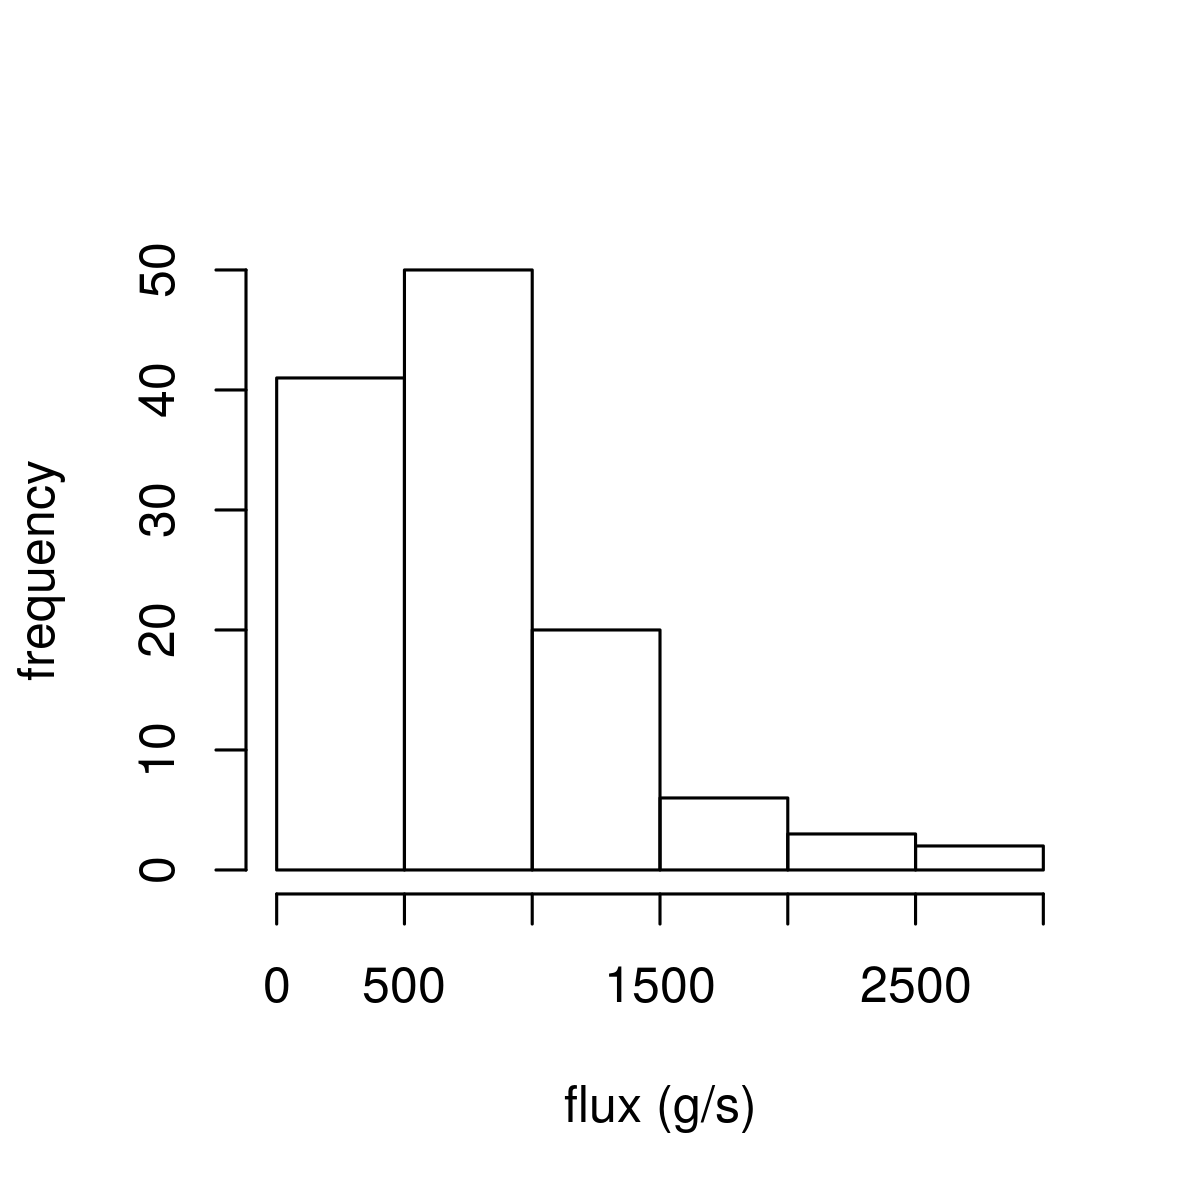
\includegraphics[width=2.0in]{histUK.png}  
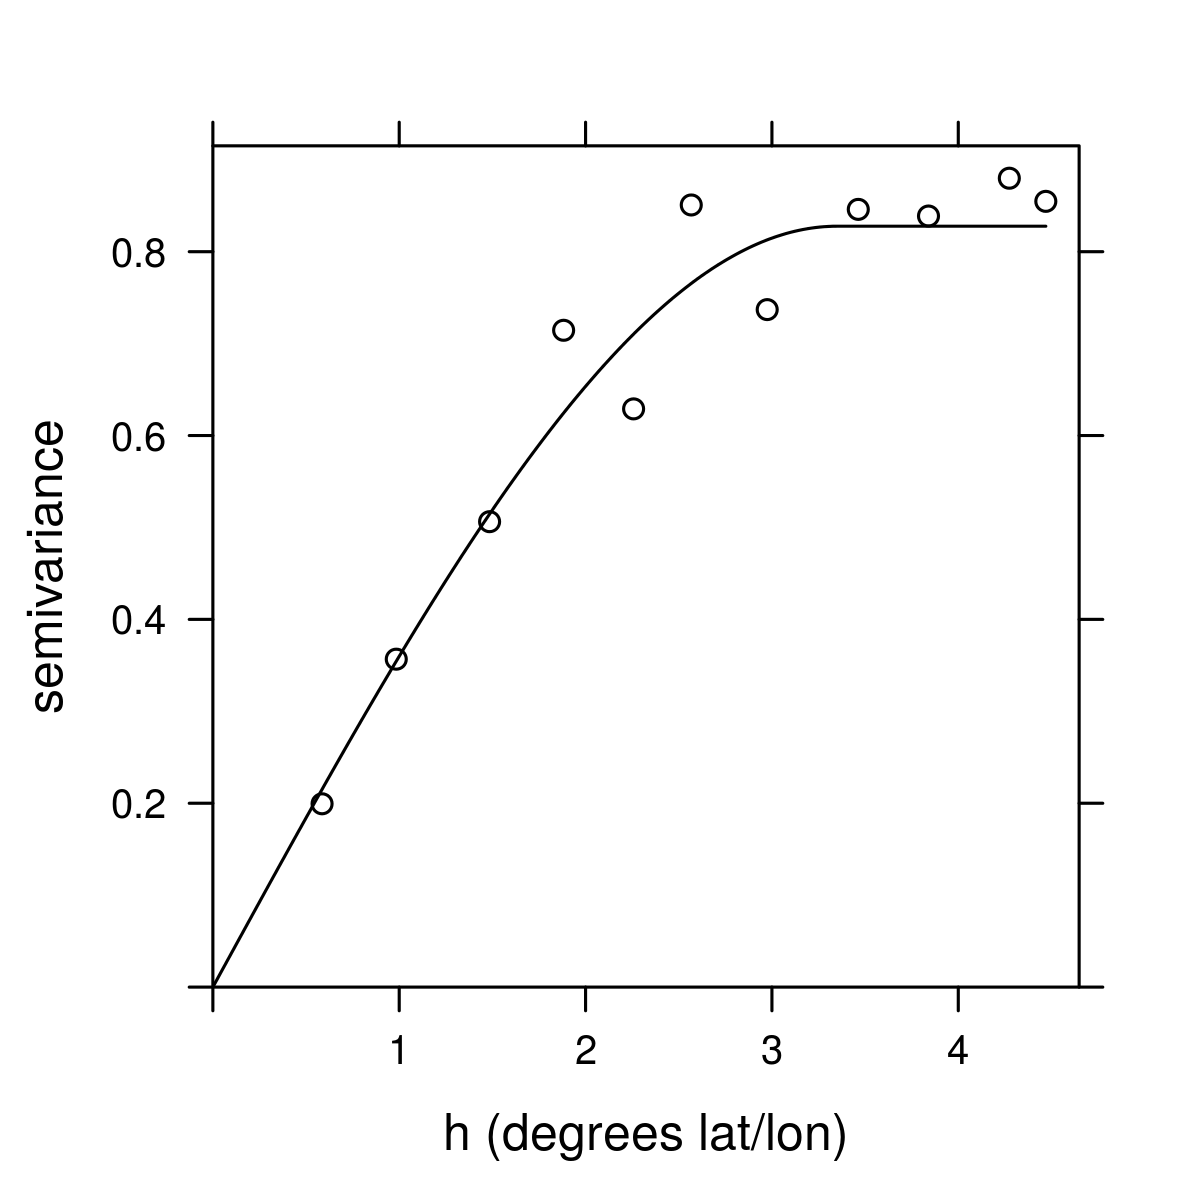
\includegraphics[width=2.0in]{variogram_est.png}  
	\caption{Histogram of NAEI fluxes in the UK and Ireland following regridding (left panel) and the empirical (open circles) and fitted (solid line) semi-variogram as a function of lag distance in degrees lat/lon. } \label{fig:var_est}
\end{figure}
\end{center}
\end{frame}

\subsection{Case study with real data}

\begin{frame}
\frametitle{UK and Ireland emissions}
\begin{itemize}
\item We used Model 1 since we only have 4 stations. \vfill
\item Laplace-EM converged in $\simeq$ 30 iterations. \vfill
\item Simulator discrepancy is not negligible: \vfill
\begin{enumerate}
\item $\hat\sigma_{2|1} \simeq 20$ ppb, \vfill
\item $\hat d \simeq 200$ km, \vfill
\item $\hat a \simeq 0.94$ ($1/e$ rate of 32 h). \vfill
\end{enumerate}
\end{itemize}
\end{frame}

\begin{frame}
\frametitle{Emissions comparison}

\begin{figure}
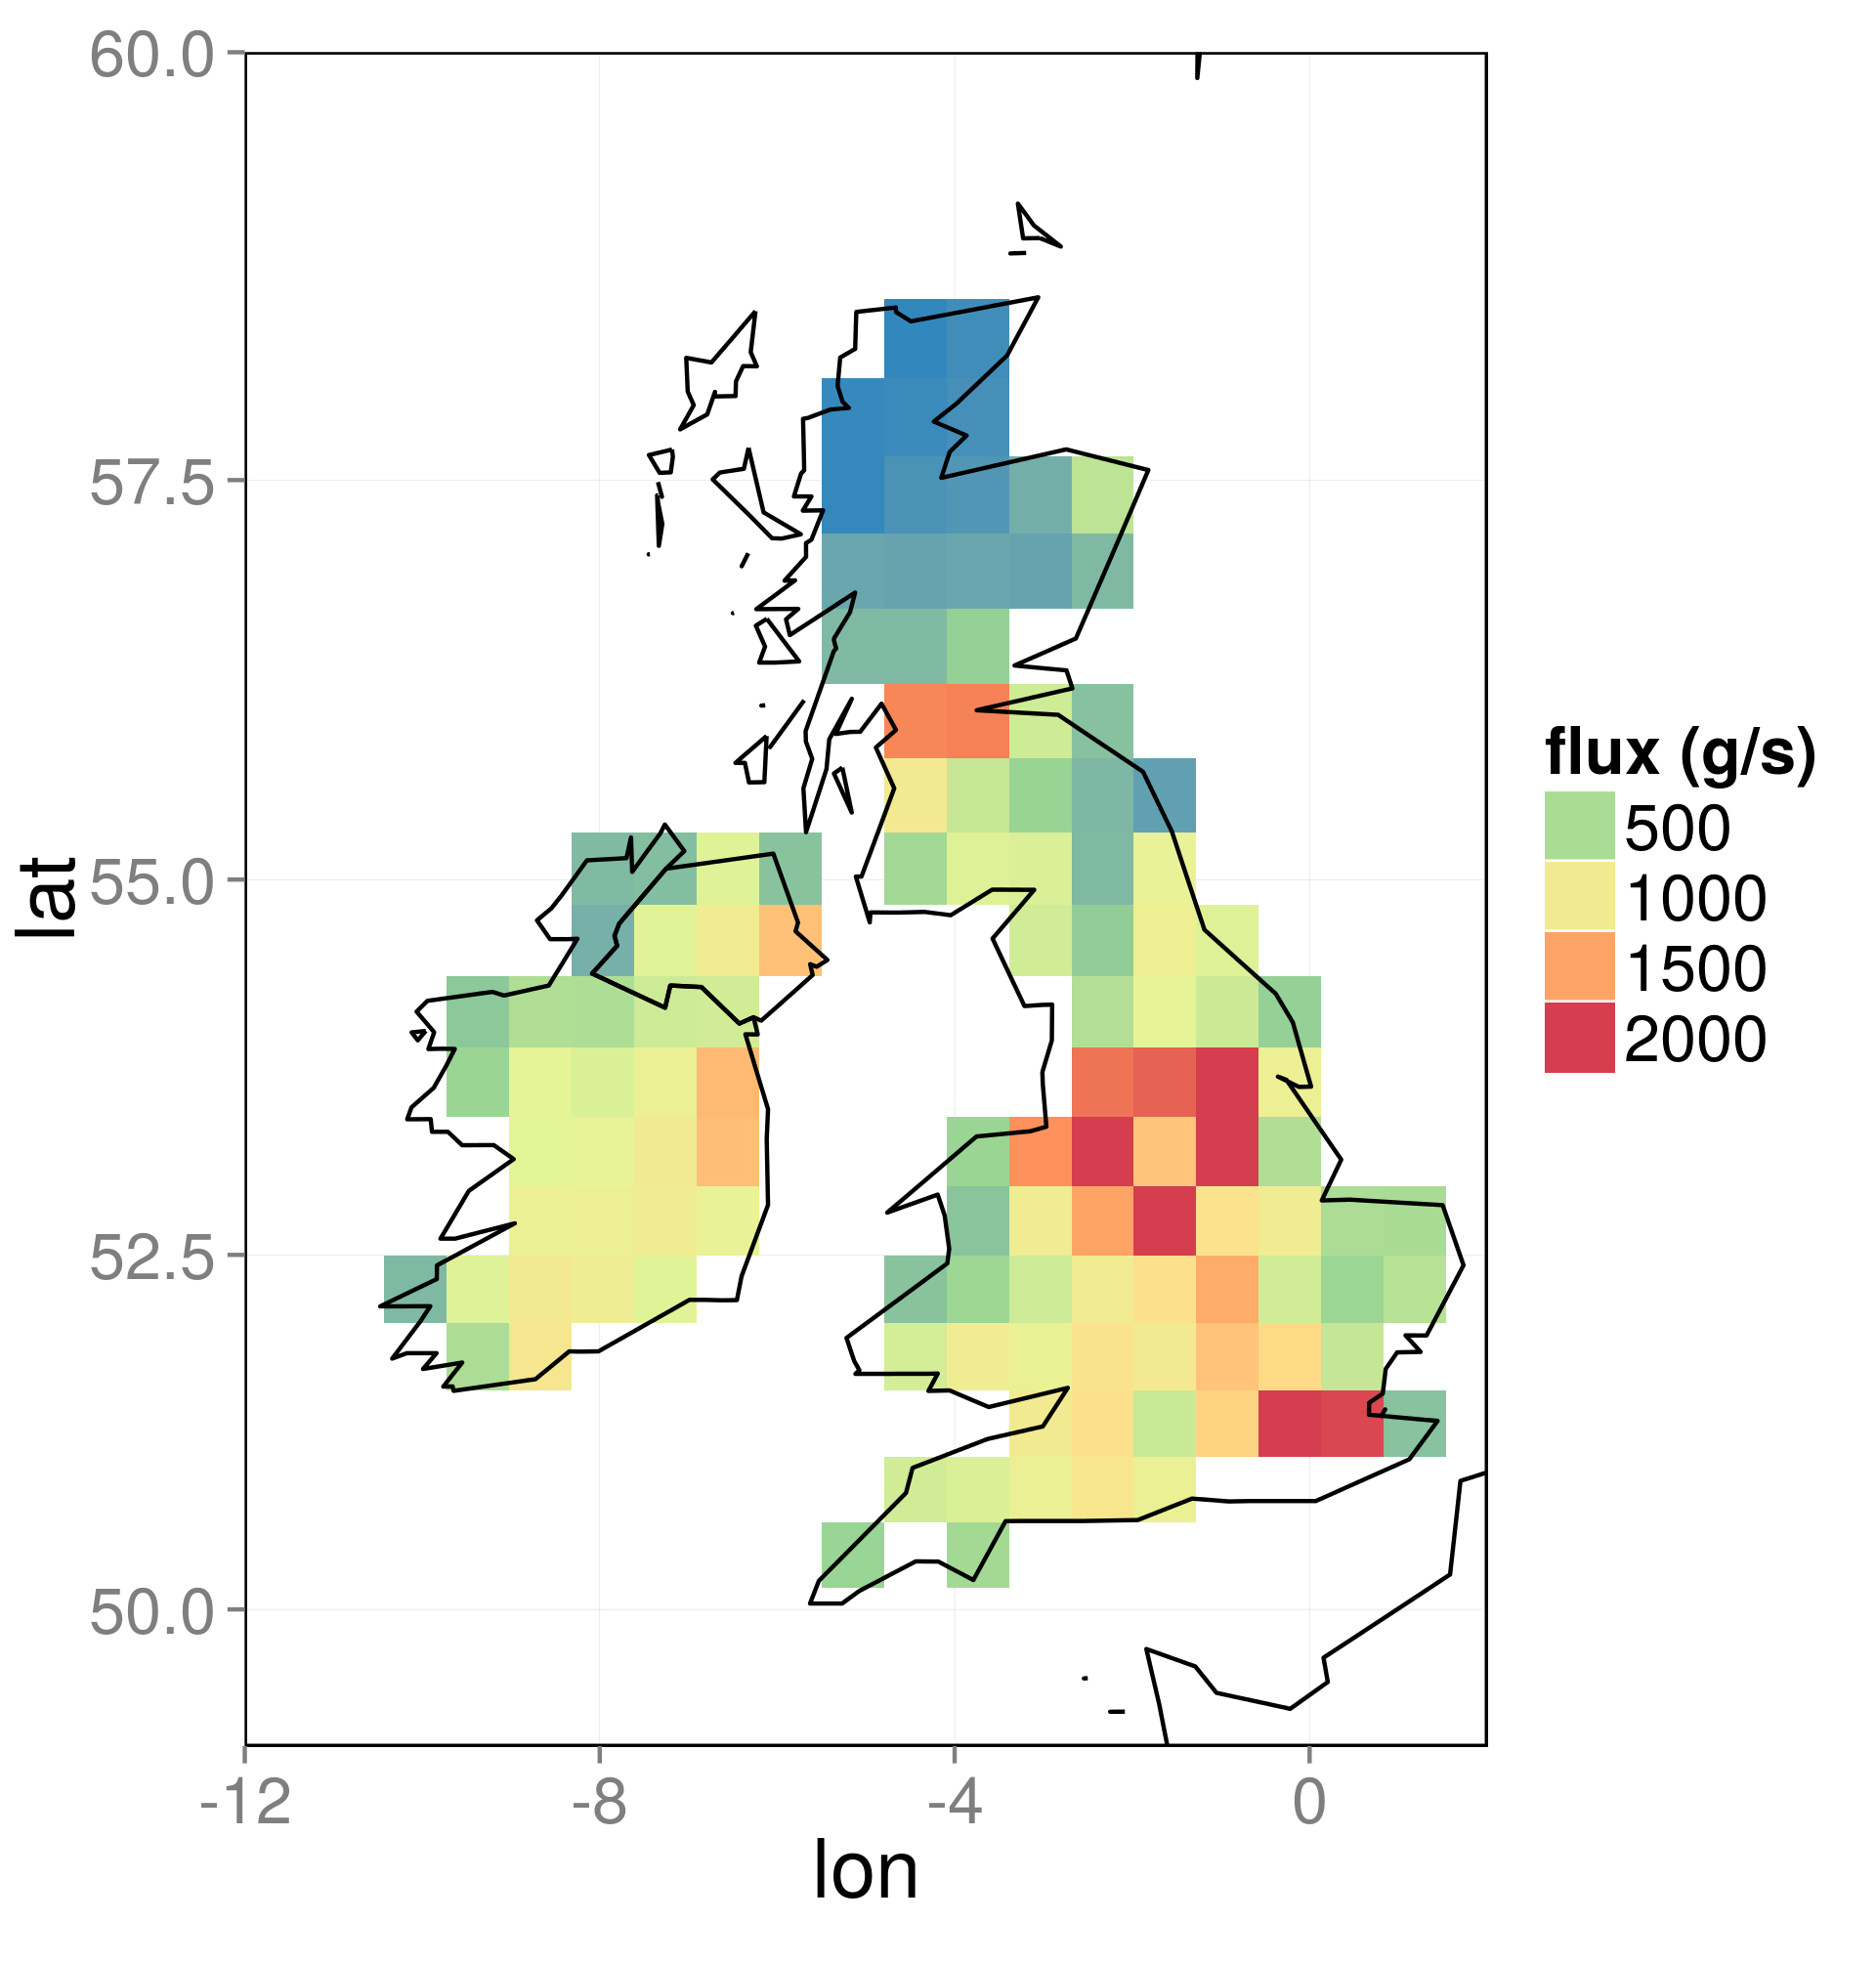
\includegraphics[width=2.0in]{NAEI_land_only.png}  
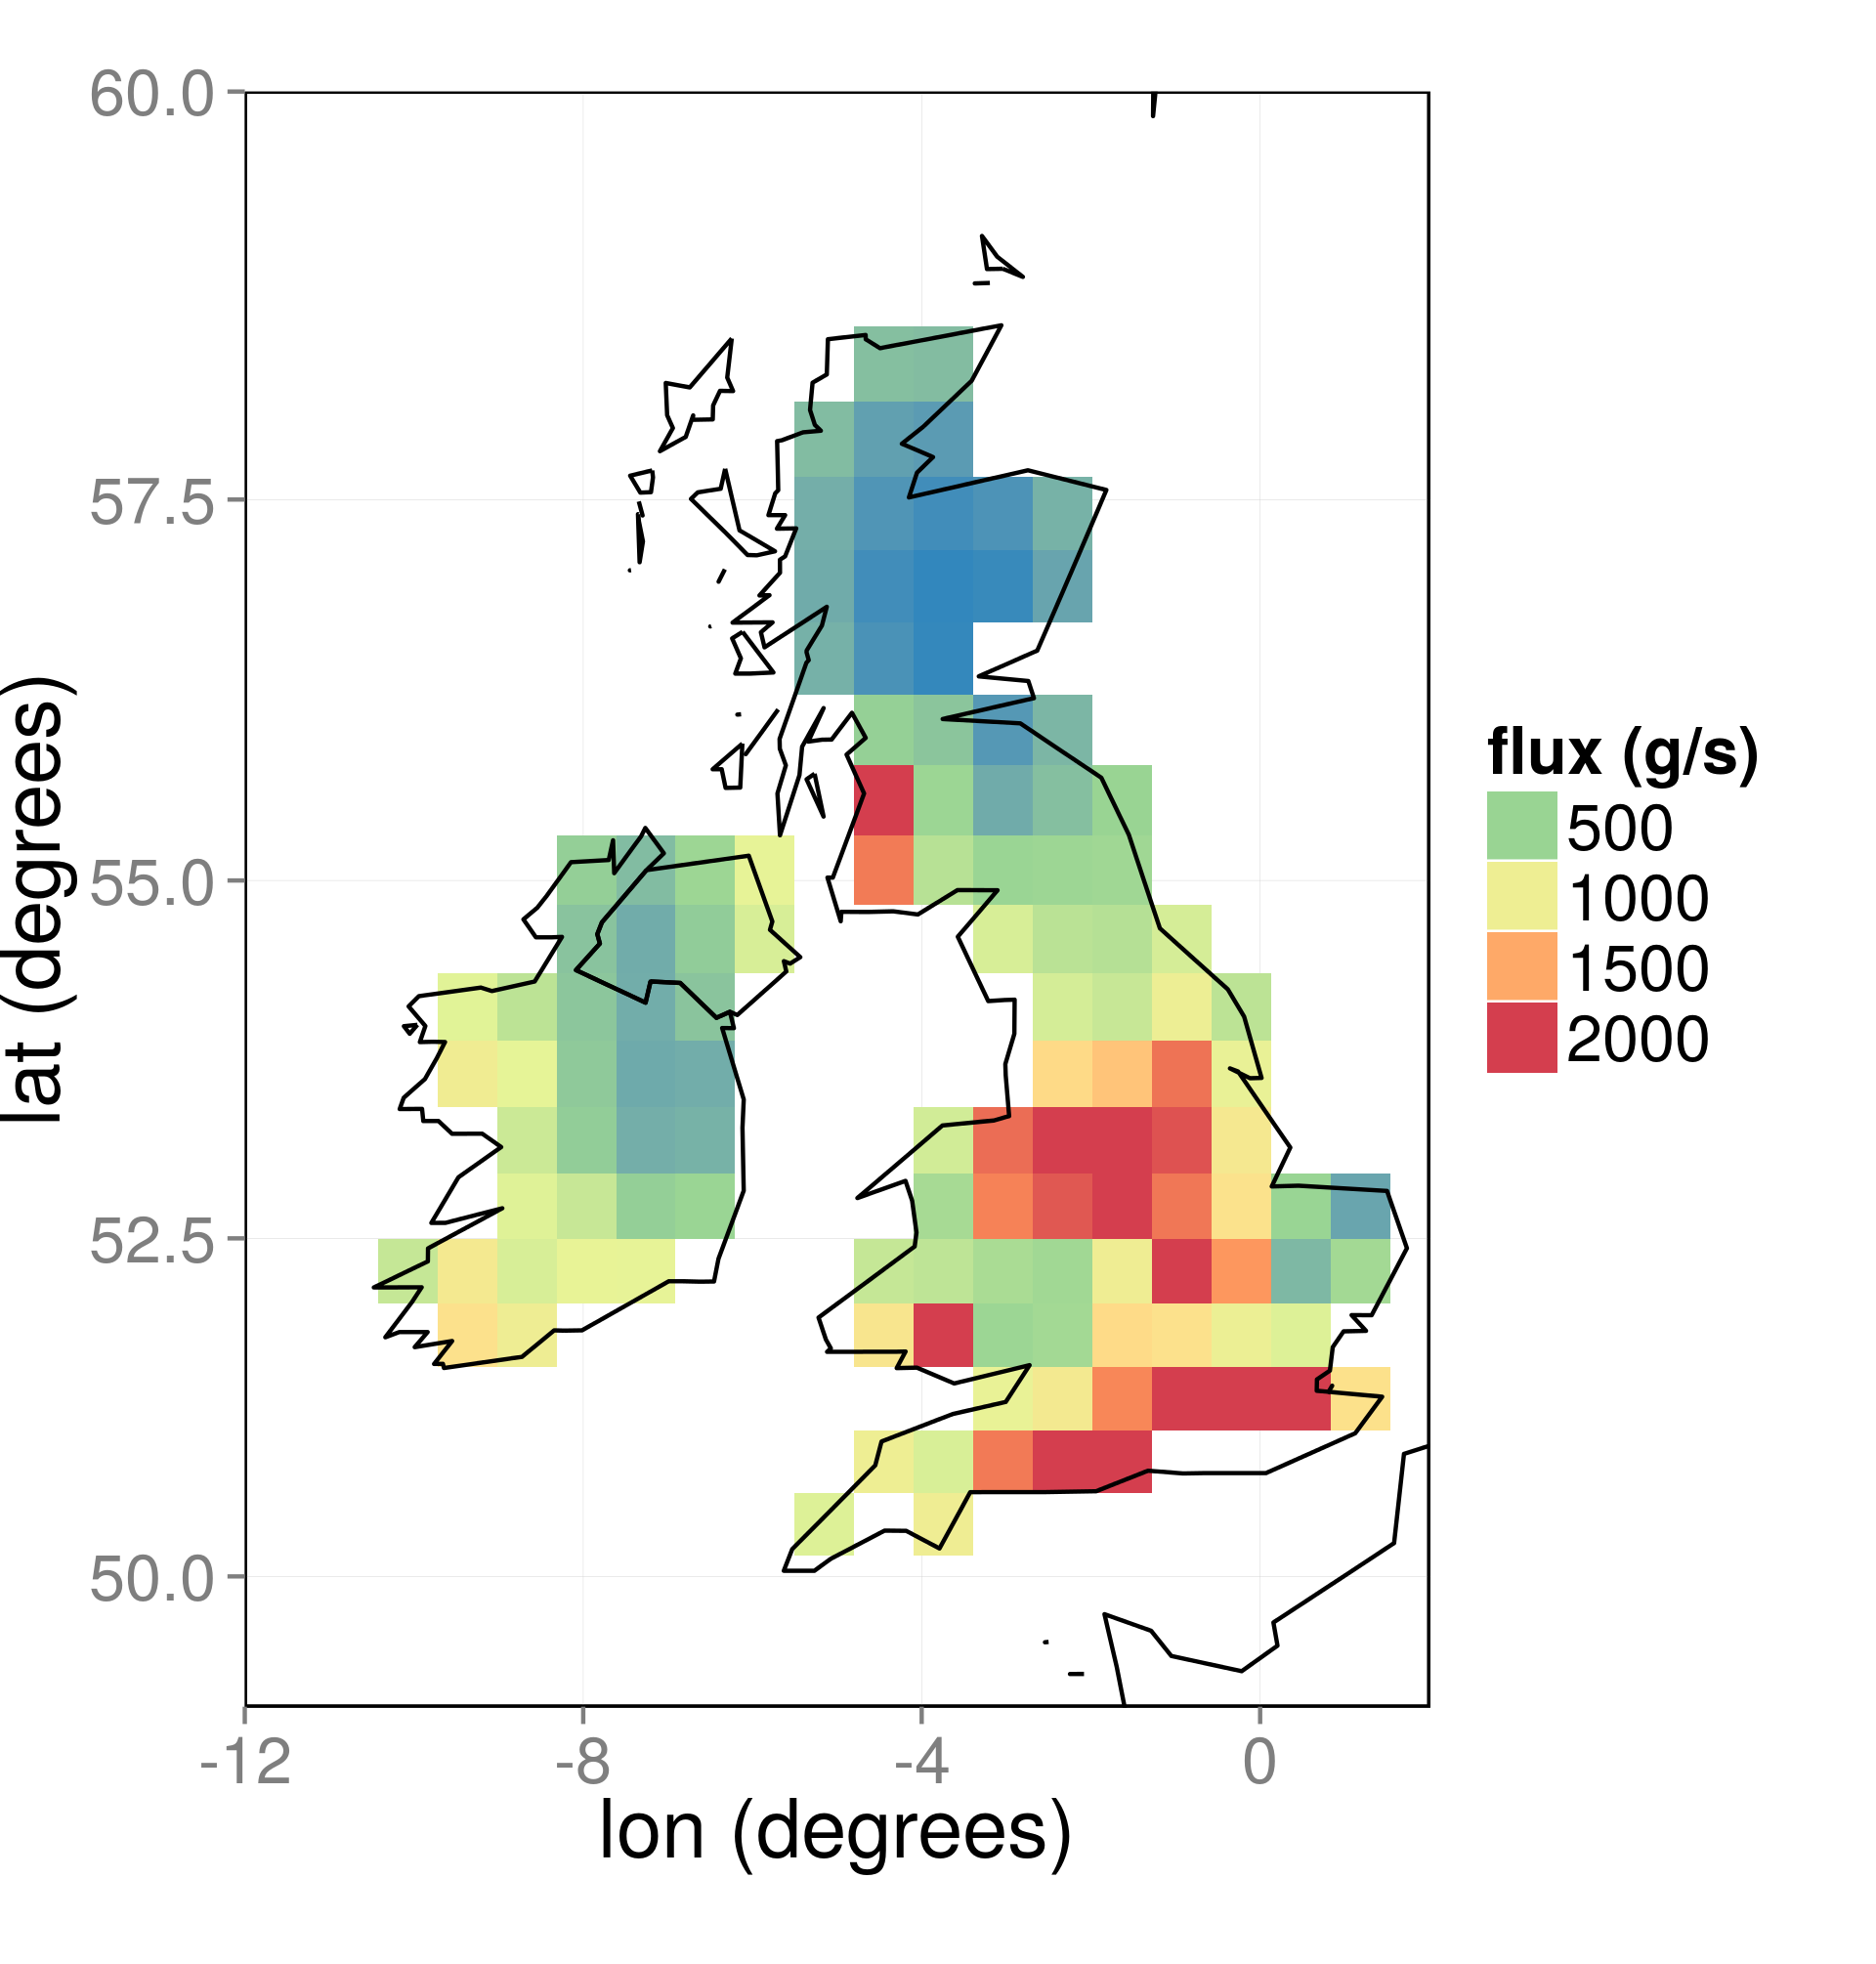
\includegraphics[width=2.0in]{Em95.png}  
	\caption{NAEI (left panel) and 95 percentile (right panel) methane emissions in the UK and Ireland, obtained using the Laplace-EM/HMC approach. Emissions in the white grid cells were treated as background emissions and used to correct the observations.}
\end{figure}
\end{frame}



\section{Conclusions}

\begin{frame}
\sectionpage
\end{frame}


\begin{frame}
\frametitle{Conclusions}

\begin{itemize}
\item Bivariate and multivariate models often appear in environmental studies. Usually, one or more of these are `explained away' prior to commencing the analysis.
\item Causal models allow for a (very) flexible model class through interaction functions that can be arbitrarily complex.
\item Computation is key: For large, non-Gaussian systems, approximate message passing + variational techniques are probably needed \citep{Cseke_2014}.
\item Slides and reproducible code available at \texttt{https://github.com/andrewzm/bicon}.
\item Thanks for Anita Ganesan and Matthew Rigby (University of Bristol) for help with the application case study.
\end{itemize}
\end{frame}

\small

\begin{frame}[allowframebreaks]
\frametitle{References}

\bibliography{../vignettes/Bibliography}


\end{frame}

\end{document}

